\documentclass[A4,12pt]{article}


\usepackage[pages=some]{background}
\usepackage{wallpaper,kantlipsum}
\usepackage{lipsum}
\usepackage{tikz}
\usetikzlibrary{shadings, calc} 
\usetikzlibrary{trees}
\usetikzlibrary{decorations.pathmorphing}
\usetikzlibrary{decorations.markings}
\usetikzlibrary{shapes.misc, positioning}
\usetikzlibrary{shapes}
\usepackage[siunitx,european]{circuitikz} %Circuits
\usetikzlibrary{arrows}
%\usepgflibrary{arrows.new}
%\usetikzlibrary{arrows.new}

\usepackage{pgfplots}
\usepgfplotslibrary{fillbetween}

\usepackage{verbatim}

\usepackage{starfont}
\usepackage{wasysym}
\usepackage{gensymb}

\usepackage{pgfplots}
\usepgfplotslibrary{fillbetween}
\pgfplotsset{compat=newest}

\definecolor{Greenss}{rgb}{0.0, 0.5, 0.0}

%\usepackage{slashbox}
\usepackage{multicol}
\usepackage{diagbox}
\usepackage{graphicx}
\usepackage{epsfig}
\usepackage{float}
\usepackage{amssymb}
\usepackage{rotating}
\usepackage{amsmath}
\usepackage{amsthm}
\usepackage{makeidx}
%\usepackage{wrapfig}
\usepackage{float}
\usepackage{color}
\usepackage{colortbl}
%\usepackage[dvipsnames]{xcolor}
\usepackage{footnote}
\usepackage{enumerate}
\usepackage{enumitem}
\usepackage{pstricks}
\usepackage{lscape}
\usepackage{colortbl}
\usepackage{bm}
\usepackage{tabularx}
\usepackage{array}
\usepackage{adjustbox}

\usepackage{subcaption}

\usepackage{bbding}  % tetexlive nuevos simbolos
\usepackage{pifont}  % nuevos simbolos$
%\usepackage{phaistos}% nuevos simbolos$
\usepackage{textcomp}% nuevos simbolos$
\usepackage{phaistos}
%\usepackage{slashbox}
\usepackage{diagbox}

\usepackage{comment}

\usepackage{mathtools}
\usepackage{animate}



\usepackage{units_carlos}


\usepackage[pdftoolbar=true,pdfmenubar=true,linkcolor=blue]{hyperref}
%
\hypersetup{ colorlinks,
linkcolor=blue,
filecolor=blue,
urlcolor=blue,
citecolor=red }
% SIZE
\voffset=-1in \hoffset=-1.5in \textwidth=18.75cm \textheight=23.5cm
\baselineskip=25pt \topmargin 1 cm \oddsidemargin 2.5cm
\evensidemargin 2.5cm \headsep=1cm
%


%\pagenumbering{nonumber}

\definecolor{GREEN}{rgb}{0.44,0.68,0.53}
\definecolor{applegreen}{rgb}{0.55, 0.71, 0.0}

% Headers ......................
\usepackage{fancyhdr}
\usepackage{lastpage}
%\pagestyle{fancy}
%\fancyhf{} 
%\fancyheadoffset{0.5 cm}
%\rfoot{\thepage/7}
%\lfoot{This copy belongs to:}
%\cfoot{{\bf Dr. Carlos Triguero}}
%\renewcommand{\headrulewidth}{0.4pt}
%\renewcommand{\footrulewidth}{0.4pt}
% Headers ......................
%
%
%
%
\usepackage[yyyy,yyyymmdd,hhmmss]{datetime}
\renewcommand{\dateseparator}{}
\renewcommand{\timeseparator}{}
\makeindex
%
%Solution environment
%Solution environment
%Solution environment
%Solution environment
%
%
%
% SHOW SOLUTION:
%
\newenvironment{solution}{\color{blue}\vspace{4mm}\\
\underline{\bf\large Solution:}\vspace{4mm}\\}{}
%
%\excludecomment{solution}
%
% HIDE SOLUTION: https://tex.stackexchange.com/questions/501698/environment-that-ignores-the-content
%
%\newenvironment{solution}{}{}
%
%
%
%
%Solution environment
%Solution environment
%Solution environment
%Solution environment
%
%
%
%Solution environment
%Solution environment
%Solution environment
%Solution environment
%
%
%
% SHOW SOLUTION:
%
\newenvironment{example}{\color{Greenss}\vspace{4mm}\\
\underline{\bf\large Worked example:}\vspace{4mm}\\}{}
%
%
% HIDE SOLUTION: https://tex.stackexchange.com/questions/501698/environment-that-ignores-the-content
%
%\newenvironment{solution}{}{}
%
%
%
%
%Solution environment
%Solution environment
%Solution environment
%Solution environment




\definecolor{Greenss}{rgb}{0.0, 0.5, 0.0}
\definecolor{GREEN}{rgb}{0.44,0.68,0.53}
\definecolor{applegreen}{rgb}{0.55, 0.71, 0.0}


\DeclareMathOperator{\foo}{foo}
\DeclareMathOperator*{\hocolim}{hocolim}



\pagestyle{fancy}
\fancyhf{}
\rfoot{\large{\thepage/\pageref{LastPage}}}
\fancyhead[L]{Motion}
\fancyhead[R]{\the\year{} Dr. C. Triguero}


\begin{document}


\title{\Huge Motion\\
\large{Yr11 Physics\\Holy Cross College}}
\date{\bf version \today\currenttime}
\maketitle


\begin{tikzpicture}
\node[draw,text width=17cm, line width=0.5mm, rounded corners=10pt, fill=yellow!50] at (0,0) % rounded rectangle
{
\begin{itemize}
\section*{\colorbox{black}{\textcolor{white}{\bf Specification CCEA Yr. 11 DA Science:}}}
    \item[\bf M1] {\bf Investigate and	use	the	quantitative	relationships between initial	speed, final speed, average speed, distance	moved, rate	of change of speed and time.}
    \item[\bf M2] {\bf calculate the	average	speed from linear distance–time graphs.}
    \item[\bf M3] {\bf define that	distance	is	measured	in	metres	(m), speed	in	metres	per	second	(m/s)	and	rate	of change	of	speed	in	metres	per	second	squared	(m/s$^2$).}
    \item[\bf M4] {\bf Recall and use the equations:
        \begin{equation*}
        \begin{split}
            & \text{Average speed}=\frac{\text{distance moved}}{\text{time taken}}\hspace{0.5cm}\text{or}\hspace{0.5cm}v=\frac{s}{t}\\
            & \text{Average speed}=\frac{\text{initial speed+final speed}}{2}\hspace{0.5cm}\text{or}\hspace{0.5cm}v=\frac{v_\text{i}+v_\text{f}}{2}\\
            &\text{Rate of change of speed}=\frac{\text{final speed-initial speed}}{\text{time taken}}\hspace{0.5cm}\text{or}\hspace{0.5cm}v=\frac{v_\text{f}-v_\text{i}}{t}\\
        \end{split}
        \end{equation*}
    }
    \item[\textcolor{GREEN}{\bf M5}] \textcolor{GREEN}{\bf \underline{Prescribed Practical P1:} use simple apparatus, including	trolleys,	ball-bearings, metre rules,	stop-clocks	and	ramps to investigate experimentally	how	the	average	speed of an	object moving	down a runway depends on the slope of the	runway	measured as the	height	of one end	of the runway (ICT	resources could	be used to	process	the	measurements and analyse the data).}
    \vspace{10mm}
\end{itemize}
};
\end{tikzpicture} 
%
%
\thispagestyle{empty}

%
\newpage

%
%
\begin{tikzpicture}
\node[draw,text width=17cm, line width=0.5mm, rounded corners=10pt, fill=yellow!50] at (0,0) % rounded rectangle
{
\begin{itemize}
\section*{Specification CCEA Yr11-Physics:}
    \item[\bf M6] {\bf demonstrate	understanding that:
    \begin{itemize}
        \item[\bf (a)] A vector is a quantity that depends on	direction and scalar	is a quantity that does	not.
        \item[\bf (b)] displacement	is	a	vector	and	that	distance	is	a	scalar	but	both	are	measured	in	metres	(m).
        \item[\bf (c)] velocity	is	a vector	and	speed is scalar but	both are measured in	metres per second (m/s).
        \item[\bf (d)] Acceleration	is a	vector	and	rate of	change of speed is	a	scalar	but	both	are	measured in metres	per	second	squared	(m/s$^2$).
    \end{itemize}
    }
    \item[\bf M7] {\bf Recall and use the	quantitative relationships between displacement, time and average velocity:
    \begin{equation*}
        \text{Average velocity}=\frac{\text{displacement}}{\text{time taken}}\hspace{0.5cm}\text{or}\hspace{0.5cm}\vec{v}=\frac{\vec{d}}{t}
    \end{equation*}
    }
    \item[\bf M8] {\bf Recall and use the	quantitative relationships between initial	velocity, final velocity,	acceleration and time:
    \begin{equation*}
        \text{Average velocity}=\frac{\text{initial velocity+final velocity}}{2}\hspace{0.5cm}\text{or}\hspace{0.5cm}\vec{v}=\frac{\vec{v}_\text{i}+\vec{v}_\text{f}}{2}
    \end{equation*}
    }
    \item[\bf M9] {\bf Recall and use the	quantitative relationships between initial	velocity, final velocity,	acceleration and time:
     \begin{equation*}
         \text{Acceleration}=\frac{\text{final velocity-initial velocity}}{\text{time taken}}\hspace{0.5cm}\text{or}\hspace{0.5cm}\vec{a}=\frac{\vec{v}_\text{f}-\vec{v}_\text{i}}{t}
     \end{equation*}
     }
     \item[\bf M10] {\bf Explain that	negative acceleration is called retardation.}
     \item[\bf M11] {\bf Use graphical methods to determine speed, distance	and	rate of change of speed, applying knowledge that:
     \begin{itemize}
         \item[\bf (a)] The	slope of a distance-time	graph is the speed
         \item[\bf (b)] The slope of	a speed–time graph is the	rate of change of speed.
         \item[\bf (c)] The	area	under a speed-time graph	is the distance moved.
     \end{itemize}	
     }
    \vspace{10mm}
\end{itemize}
};
\end{tikzpicture} 
     \newpage

%
%
\begin{tikzpicture}
\node[draw,text width=17cm, line width=0.5mm, rounded corners=10pt, fill=yellow!50] at (0,0) % rounded rectangle
{
\begin{itemize}
\section*{Specification CCEA Yr11-Physics:}
     \item[\bf M12] {\bf Use graphical methods to determine velocity, acceleration and	displacement, applying knowledge that:
     \begin{itemize}
         \item[\bf (a)] The	slope	of a displacement-time	graph is the velocity.
         \item[\bf (b)] The	slope of a velocity–time	graph is the acceleration.
         \item[\bf (c)] The area under a velocity-time graph is the displacement.
     \end{itemize}	
     }
    \vspace{10mm}
\end{itemize}
};
\end{tikzpicture} 
%
%
%
%
%
%
%
%
\newpage
\section*{Main equations:}

\vspace{-5 mm}

\begin{table}[H]
    \centering
    \scalebox{1.3}{
    \begin{tabular}{|lr|}\hline 
     \rowcolor{yellow}{
    {\bf Motion:}&}
    \\\hline
    \rowcolor{gray!50}{
    {\bf Studied motions:} One dimensional motions. Straight line motion.}
    &\\\hline
    \rowcolor{white}{
    {\bf UM: Uniform Motion (constant velocity)}}
    &\\
    \rowcolor{white}{
    {\bf UAM: Uniformly Accelerated Motion (constant acceleration)}}
    &\\\hline
    \rowcolor{gray!50}{
    {\bf Variable definition:}}
    &\\\hline
    {\bf Distance,} $\bm{d:}$ Quantity of space between two points along a path.&\\
    {\bf Displacement,} $\bm{\vec{d}:}$ Relative distance and direction between two positions. &\\
    {\bf Average speed,} $\bm{v:}$ Increment of the distance per time unit. &\\
    {\bf Average velocity,} $\bm{\vec{v}:}$ Increment of the displacement per time unit. &\\
    {\bf Rate of change of speed,} $\bm{a:}$ Increment of the average speed per time unit. &\\
    {\bf Average acceleration,} $\bm{a:}$ Increment of the average velocity per time unit. &\\\hline
    %
    %
    %
    %
    %
    \rowcolor{yellow}{
    {\bf SCALAR VARIABLES: Average speed $\bm v$ relations:}}
    &\\\hline
     \rowcolor{blue!20}{\bf Average speed - distance - time} \textcolor{red}{\bf It can be used always}    &  \\
     %
     \vspace{-1.5 mm}
     \begin{tikzpicture}[thick,scale=1.0, every node/.style={transform shape}]
    \draw[rounded corners=10mm,draw=black,line width = 0.75mm,fill=yellow] (0,0) -- (3,0) -- (1.5,2.5) --cycle;
    \draw[line width = 0.5mm] (0.75,1) -- (2.25,1);
    \node[at={(1.5,0.5)},color=black]{\Huge $v\times t$};
    \node[at={(1.5,1.5)},color=black]{\Huge $d$};
    \node[right] at (3,1.7) {$\bm{d}$ is the distance. S.I. unit metre, m.};
    \node[right] at (3,1) {$\bm v$ is the speed. S.I. unit m/s.};
    \node[right] at (3,0.3) {$\bm{t}$ is the time taken. S.I. unit second, s.};
    \node[right] at (-3,1) {$\displaystyle{\bm{v=\frac{d}{t}}}$};
    \end{tikzpicture} &
     %
     \\
     \rowcolor{red!20}{\bf Average speed - initial speed - final speed:}  & \\
     $\displaystyle{\bm{v=\frac{v_\text{i}+v_\text{f}}{2}}}$ \hspace{1cm} Can be used \textcolor{red}{only} for UM or UAM & \\
     \rowcolor{gray!20}{\bf Rate of change of speed - initial and final speed - time:}    &  \\
     $\displaystyle{\bm{ a=\frac{v_\text{f}-v_\text{i}}{t}}}$ \hspace{1cm} It is just the module of acceleration. Always valid. & \\\hline
     \rowcolor{yellow}{
    {\bf VECTORIAL VARIABLES: Average velocity $\bm{\vec{v}}$ relations:}}
    &\\\hline
     \rowcolor{blue!20}{\bf Average velocity - displacement - time: \textcolor{red}{\bf It can be used always}}    &  \\
     %
     %
     %
      %
     \vspace{-1.5 mm}
     \begin{tikzpicture}[thick,scale=1.0, every node/.style={transform shape}]
    \draw[rounded corners=10mm,draw=black,line width = 0.75mm,fill=yellow] (0,0) -- (3,0) -- (1.5,2.5) --cycle;
    \draw[line width = 0.5mm] (0.75,1) -- (2.25,1);
    \node[at={(1.5,0.5)},color=black]{\Huge $\vec{v}\times t$};
    \node[at={(1.5,1.5)},color=black]{\Huge $\vec{d}$};
    \node[right] at (3,1.7) {$\bm{\vec{d}}$ is the displacement. S.I. unit metre, m.};
    \node[right] at (3,1) {$\bm{\vec{v}}$ is the velocity. S.I. unit m/s.};
    \node[right] at (3,0.3) {$\bm{t}$ is the time taken. S.I. unit second, s.};
    \node[right] at (-3,1) {$\displaystyle{\bm{\vec{v}=\frac{\vec{d}}{t}}}$};
    \end{tikzpicture} &\\
     \rowcolor{red!20}{\bf Average velocity - initial velocity - final velocity:}    &  \\
     $\displaystyle{\bm{\vec{v}=\frac{\vec{v}_\text{i}+\vec{v}_\text{f}}{2}}}$ \hspace{1cm} Can be used \textcolor{red}{only} for UM or UAM & \\
     {\rowcolor{gray!20}\bf Average acceleration - initial and final velocity - time:}    &  \\
     $\displaystyle{\bm{ \vec{a}=\frac{\vec{v}_\text{f}-\vec{v}_\text{i}}{t}}}$ \hspace{1cm} Can be used always & \\\hline
    \end{tabular}}
\end{table}

%
\newpage

\begin{figure}[H]
    \centering
    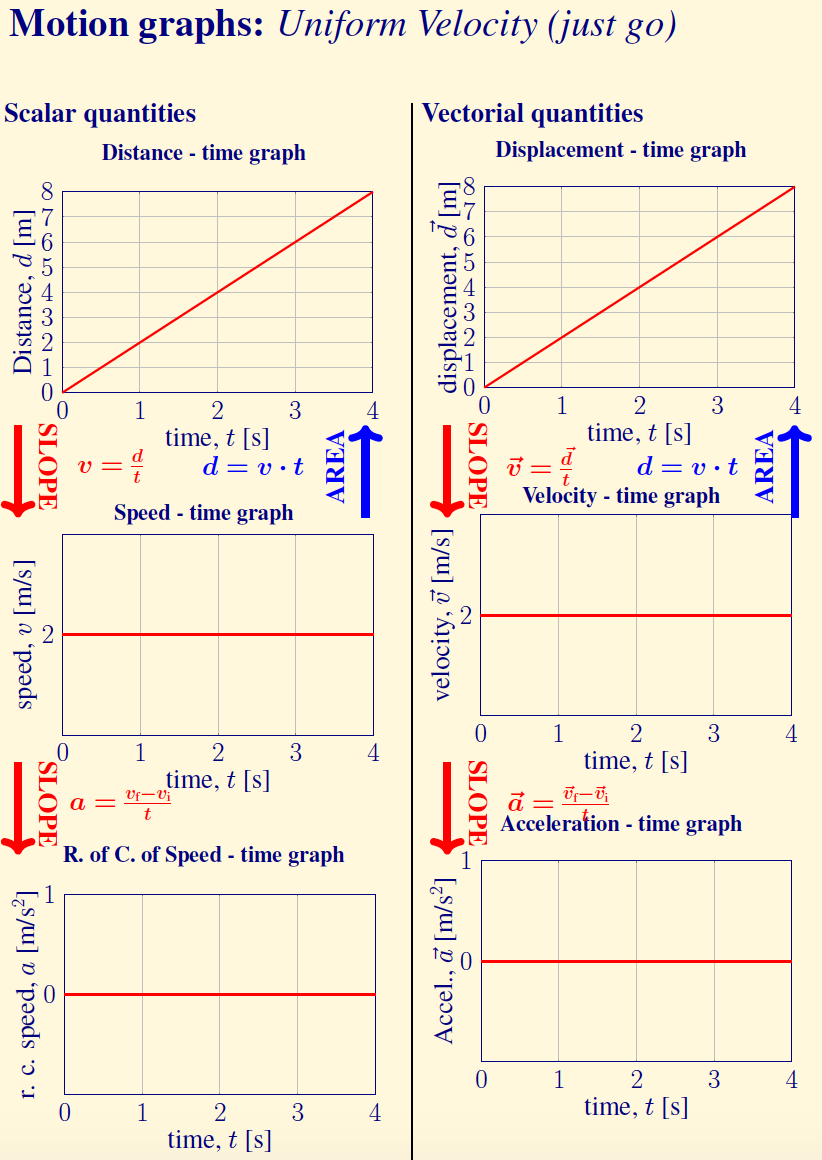
\includegraphics[scale=1.1]{FIG1.png}
\end{figure}

\newpage

\begin{figure}[H]
    \centering
    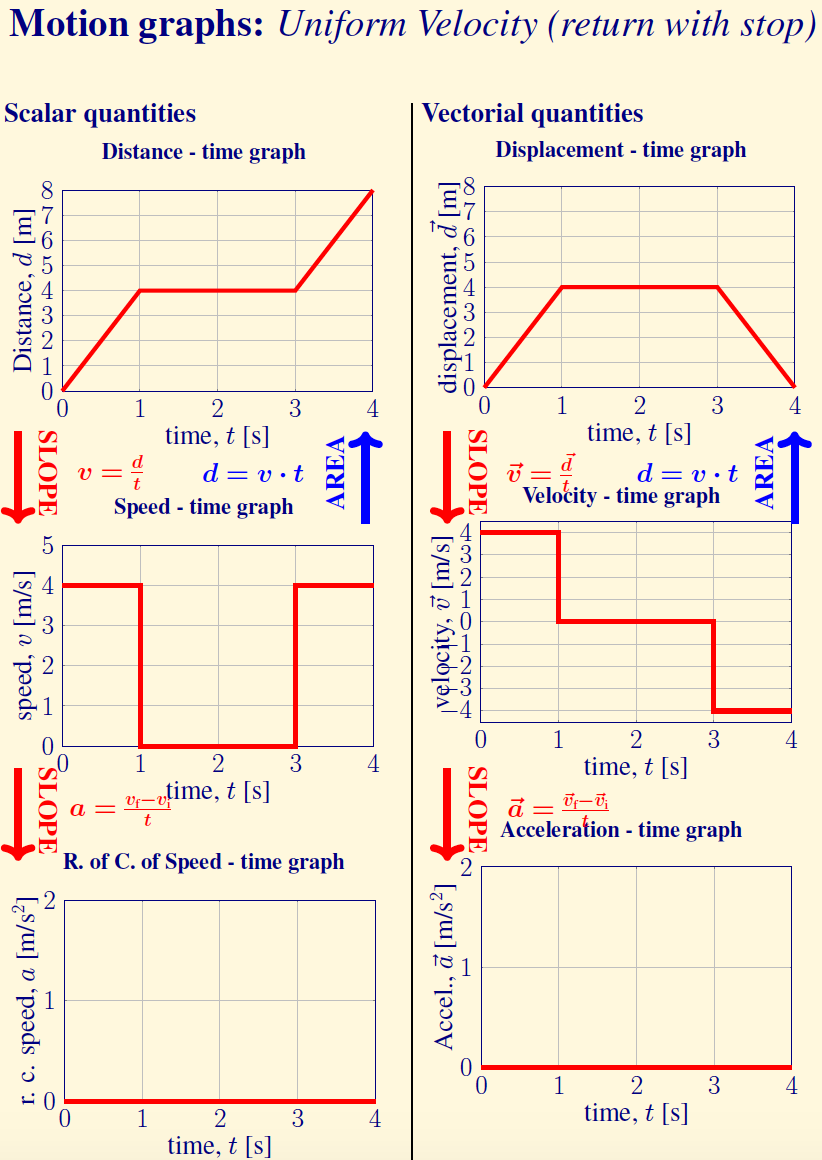
\includegraphics[scale=1.1]{FIG2.png}
\end{figure}

\newpage

\begin{figure}[H]
    \centering
    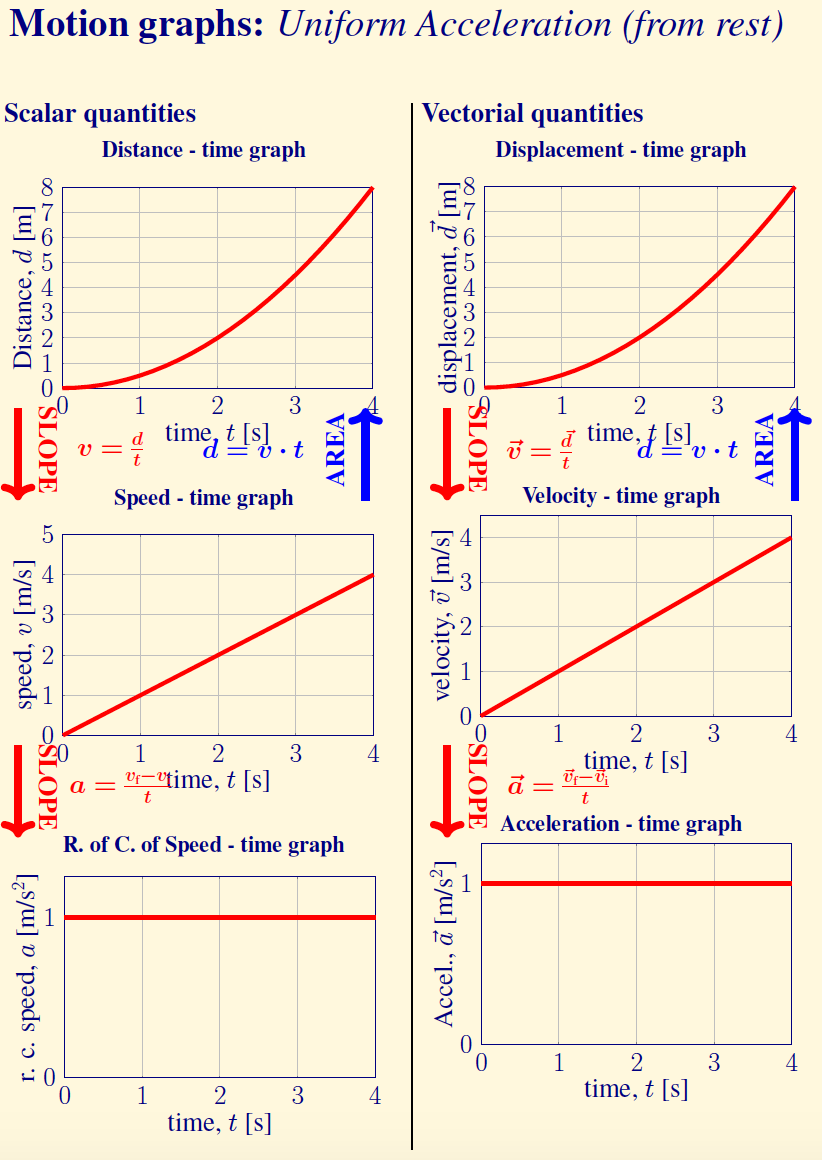
\includegraphics[scale=1.1]{FIG3.png}
\end{figure}

\newpage

\begin{figure}[H]
    \centering
    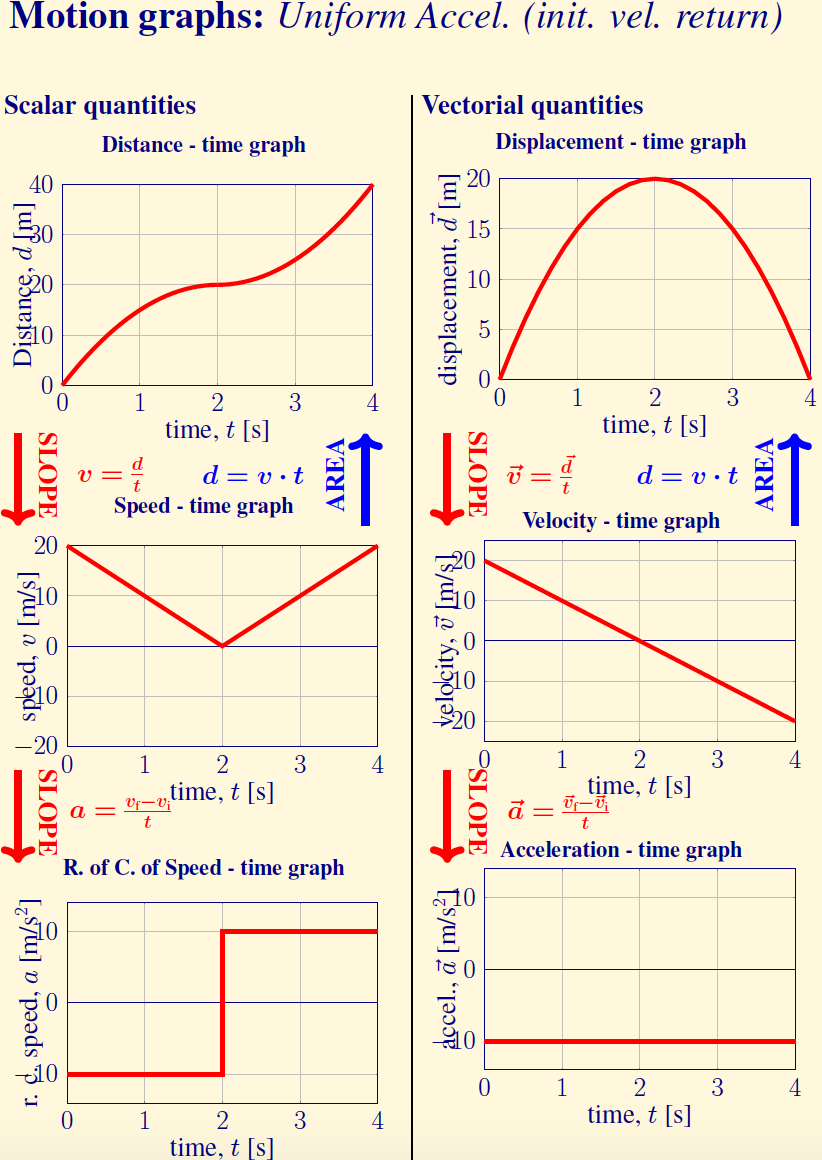
\includegraphics[scale=1.1]{FIG4.png}
\end{figure}

\newpage


\begin{enumerate}[label=\bfseries (\arabic*)]


\section*{\textcolor{red}{Position, distance and displacement:}}


% \href{https://www.nagwa.com/en/worksheets/530139601254/}{Lesson Worksheet: Position, Displacement, and Distance}\\

% \href{https://www.nagwa.com/en/worksheets/305148596864/}{Lesson Worksheet: Distance and Displacement}\\







\item A model of an electric car, the \textit{Tesla-Strabane-Xmax}, can travel \textbf{400 miles} before it needs to be recharged. \textbf{What} kind of \textbf{quantity} is the \textbf{range} of this model of car? \cite{Nagwa} \href{https://www.nagwa.com/en/worksheets/530139601254/}{Q. 20 Lesson Worksheet: Position, Displacement, and Distance}
%
\begin{multicols}{2}
\begin{itemize}
    \item[A.] Velocity
    %\item[\textcolor{blue}{\bf B.}]
    \textcolor{blue}{\bf Distance}
    \item[\bf B.] Distance
    \item[C.] Direction
    \item[D.] Displacement
    \item[E.] Speed
    \item[F.] Position
\end{itemize}
\end{multicols}








\item What kind of \textbf{information} does this signpost show? \cite{Nagwa} Q. 2 Lesson Worksheet: Position, Displacement, and Distance
%
\begin{figure}[H]
    \centering
    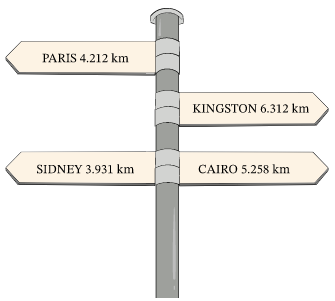
\includegraphics[width=0.4\textwidth]{Nagwa_Q2_D.png}
\end{figure}
%
\begin{multicols}{4}
\begin{itemize}
    \item[A.] Distance
    \item[B.] Velocity
    %\item[\textcolor{blue}{\bf C.}] \textcolor{blue}{\bf Displacement}
    \item[C.] Displacement
    \item[D.] Speed
\end{itemize}
\end{multicols}







\item You traveled \textbf{213 miles} from \textbf{California} to \textbf{San Francisco}. Does the ``213 miles" represent \textbf{distance} or \textbf{displacement}? \cite{Nagwa} Q. 14 Lesson Worksheet: Position, Displacement, and Distance
%
\begin{multicols}{2}
\begin{itemize}
    \item[A.] Displacement
    \item[B.] Distance
    %\item[\textcolor{blue}{\bf B.}] \textcolor{blue}{\bf Distance}
\end{itemize}
\end{multicols}












\item If you were \textbf{lost} in a forest, would you prefer to know your \textbf{distance} or your \textbf{displacement} from the nearest settlement? \cite{Nagwa} Q. 15 Lesson Worksheet: Position, Displacement, and Distance
%
\begin{multicols}{2}
\begin{itemize}
    \item[A.] Distance
    \item[B.] Displacement
    %\item[\textcolor{blue}{\bf B.}] \textcolor{blue}{\bf Displacement}
\end{itemize}
\end{multicols}










\item What is the name of the \textbf{vector} quantity which gives the \textbf{total change of a particle’s position}? \cite{Nagwa} Q. 3 Lesson Worksheet: Position, Displacement, and Distance
%
\begin{multicols}{2}
\begin{itemize}
    \item[A.] Distance
    \item[B.] Acceleration vector
    \item[C.] Displacement
    %\item[\textcolor{blue}{\bf C.}] \textcolor{blue}{\bf Displacement}
    \item[D.] Velocity vector
\end{itemize}
\end{multicols}














\item \label{Pos}Indicate the \textbf{displacement} of the different dots with respect to the \textbf{position 0} over the axis (number in cm). \textcolor{gray}{[SPEC M3]} \cite{Triguero}\\
\textcolor{gray}{Help: Displacement can be a negative real number.}
% With ruler better?

\begin{figure}[H]
    \centering
    \begin{tikzpicture}
     \draw[gray,line width=0.5mm] (-7,0)--(7,0);
      \foreach \i in {-7,...,7} {
        \draw[gray,line width=0.5mm] (\i,0)--(\i,-0.35);
        \node [below] at (\i,-0.35) {$\i$}
        }
        %\node[at={(8,0)},color=black]{$\vec{d}=$};
        \node[at={(8,0)},color=blue]{$\bm{\vec{d}=+3}$};
        \filldraw[black] (3,0) circle (1.25mm);
    \end{tikzpicture}\\
    \vspace{0.5cm}
    \begin{tikzpicture}
     \draw[gray,line width=0.5mm] (-7,0)--(7,0);
      \foreach \i in {-7,...,7} {
        \draw[gray,line width=0.5mm] (\i,0)--(\i,-0.35);
        \node [below] at (\i,-0.35) {$\i$}
        }
        %\node[at={(8,0)},color=black]{$\vec{d}=$};
        \node[at={(8,0)},color=blue]{$\bm{\vec{d}=-5}$};
        \filldraw[black] (-5,0) circle (1.25mm);
    \end{tikzpicture}
    \caption{Displacement of different dots. Problem~\ref{Pos}.}
    \label{fig:my_label}
\end{figure}


















\item \label{Posdis} For each of the following two figures: \textcolor{gray}{[SPEC M3]} \cite{Triguero}
%
%
\begin{figure}[H]
    \centering
    \begin{tikzpicture}
     \draw[gray,line width=0.5mm,dashed] (-7,0)--(7,0);
    \draw[gray,line width=0.5mm] (0,0)--(0,-0.35);
    \node [below] at (0,-0.35) {$0$};
    %  \foreach \i in {-7,...,7} {
    %     \draw[gray,line width=0.5mm] (\i,0)--(\i,-0.35);
    %     \node [below] at (\i,-0.35) {$\i$}
    %     }
    %\node[at={(8,0)},color=black]{$P=$};
    \draw[red,fill] (2,0) circle [radius=0.3] node {\textcolor{white}{\bf A}};
    \draw[red,fill] (4.5,0) circle [radius=0.3] node {\textcolor{white}{\bf B}};
    \end{tikzpicture}
    \\
    \vspace{0.5cm}
    \begin{tikzpicture}
     \draw[gray,line width=0.5mm,dashed] (-7,0)--(7,0);
    \draw[gray,line width=0.5mm] (0,0)--(0,-0.35);
     \node [below] at (0,-0.35) {$0$};
    %  \foreach \i in {-7,...,7} {
    %     \draw[gray,line width=0.5mm] (\i,0)--(\i,-0.35);
    %     \node [below] at (\i,-0.35) {$\i$}
    %     }
    %\node[at={(8,0)},color=black]{$P=$};
    \draw[red,fill] (-3,0) circle [radius=0.3] node {\textcolor{white}{\bf A}};
    %
    \draw[red,fill] (6,0) circle [radius=0.3] node {\textcolor{white}{\bf B}};
    \end{tikzpicture}
    \caption{Displacement of different dots. Problem~\ref{Posdis}.}
    \label{fig:my_label}
\end{figure}
%
\begin{itemize}
    \item[\bf (a)] Use a ruler to give the \textbf{displacement} of the \textbf{point A} with respect to the \textbf{reference 0} over the axis.
    \item[\bf (b)] Use a ruler to give the \textbf{displacement} of the \textbf{point B} with respect to the \textbf{reference 0} over the axis.
    \item[\bf (c)] \textbf{Measure} the \textbf{distance} between \textbf{A} and \textbf{B}.
    %\item[\bf (d)] Find the \textbf{distance} between \textbf{A} and \textbf{B} using only the measured displacements for \textbf{A} and \textbf{B}.\\
     %\textcolor{gray}{Help: distance=absolute value of $\vec{d}_B$ and $\vec{d}_A$. Comment: Distance is always a positive quantity.}
     \item[\bf (d)] \textbf{Check} that the \textbf{distance} between \textbf{A} and \textbf{B} can be obtained using the measured displacements for \textbf{A} and \textbf{B} doing the following,
     \begin{equation*}
         \text{Distance from $A$ to $B$}=|\text{displacement B}-\text{displacement A}|
     \end{equation*}
     \item[\bf (e)] \textbf{Measure} the displacement of \textbf{point B} with respect to \textbf{point A} and check that the number found is equal to the \textbf{distance} between \textbf{A} and \textbf{B}. 
\end{itemize}













% BEGIN ANT PROBLEM ANIMATION:
%
\newcommand{\ant}[1]{
% Ghost point to maintain graph size
\draw[white] (0,0) circle (0ex);
\draw[white] (4.5,0) circle (0ex);
\draw[white] (0,-4.5) circle (0ex);
%
% Background Gray Trajectory
%
\draw[gray,smooth,dashed] plot[parametric,domain=0:2*pi,samples=40,line width=0.6mm] function {2*t,2.8*sin(t)};
%
% Moving Trajectory
%
\draw[red,smooth,thick] plot[parametric,domain=0:#1,samples=10*#1,line width=0.6mm] function {2*t,2.8*sin(t)};
%
% Moving Ant
%
\draw[black,smooth,thick] plot[parametric,domain=#1:#1,samples=1,mark=*,mark size=1mm] function {2*t,2.8*sin(t)};
\draw[black,smooth,thick] plot[parametric,domain=#1:#1,samples=1,mark=*,mark size=1mm] function {2*t+0.1,2.8*sin(t+0.1)};
% STARTING POINT
\draw[red,fill] (0,0) circle [radius=0.3] node {\textcolor{white}{\bf A}};
% END POINT
\draw[red,fill] (12.6,0) circle [radius=0.3] node {\textcolor{white}{\bf B}};
}
%
% END ANT PROBLEM ANIMATION:
%
%
%
%
%
%
%
% Problem starts:
%
\item Given the following path followed by an ant: \cite{Triguero} \textcolor{gray}{[SPEC Mx]}
%
\begin{center}
  \begin{animateinline}[autoplay,loop,
    begin={\begin{tikzpicture}[scale=1.0]},
    end={\stepcounter{cnt}\end{tikzpicture}}
    ]{15}
    %
    %
    \ant{6.2}\newframe
    \ant{0.0}\newframe
    \ant{0.1}\newframe
    \ant{0.2}\newframe
    \ant{0.3}\newframe
    \ant{0.4}\newframe
    \ant{0.5}\newframe
    \ant{0.6}\newframe
    \ant{0.7}\newframe
    \ant{0.8}\newframe
    \ant{0.9}\newframe
    \ant{1.0}\newframe
    \ant{1.1}\newframe
    \ant{1.2}\newframe
    \ant{1.3}\newframe
    \ant{1.4}\newframe
    \ant{1.5}\newframe
    \ant{1.6}\newframe
    \ant{1.7}\newframe
    \ant{1.8}\newframe
    \ant{1.9}\newframe
    \ant{2.0}\newframe
    \ant{2.1}\newframe
    \ant{2.2}\newframe
    \ant{2.3}\newframe
    \ant{2.4}\newframe
    \ant{2.5}\newframe
    \ant{2.6}\newframe
    \ant{2.7}\newframe
    \ant{2.8}\newframe
    \ant{2.9}\newframe
    \ant{3.0}\newframe
    \ant{3.1}\newframe
    \ant{3.2}\newframe
    \ant{3.3}\newframe
    \ant{3.4}\newframe
    \ant{3.5}\newframe
    \ant{3.6}\newframe
    \ant{3.7}\newframe
    \ant{3.8}\newframe
    \ant{3.9}\newframe
    \ant{4.0}\newframe
    \ant{4.1}\newframe
    \ant{4.2}\newframe
    \ant{4.3}\newframe
    \ant{4.4}\newframe
    \ant{4.5}\newframe
    \ant{4.6}\newframe
    \ant{4.7}\newframe
    \ant{4.8}\newframe
    \ant{4.9}\newframe
    \ant{5.0}\newframe
    \ant{5.1}\newframe
    \ant{5.2}\newframe
    \ant{5.3}\newframe
    \ant{5.4}\newframe
    \ant{5.5}\newframe
    \ant{5.6}\newframe
    \ant{5.7}\newframe
    \ant{5.8}\newframe
    \ant{5.9}\newframe
    \ant{6.0}\newframe
    \ant{6.1}\newframe
    \ant{6.2}\newframe
    \ant{6.3}\newframe
  \end{animateinline}
  \end{center}
%
\begin{itemize}
    \item[\bf (a)] \textbf{Measure} the \textbf{distance} (over the path) between the starting position \textbf{A} and the final position \textbf{B} of the ant.\\
    \textcolor{gray}{Help: Use a piece of string and a ruler.}
    %
    \item[\bf (b)] What is the \textbf{displacement} between \textbf{A} and \textbf{B}. For this give the module of the displacement and indicate the direction drawing and arrow in the figure starting at the initial point \textbf{A}.
\end{itemize}





















\item Mohammed and Maisie started walking from the \textbf{same point}. Mohammed walked \textbf{1 mile southwest} and then \textbf{3 miles northwest}. Maisie walked \textbf{4 miles northwest}, then \textbf{1 mile southwest}, and finally \textbf{1 mile southeast}. What can you say about \textbf{where they ended up}? \cite{Nagwa} Q. 17 Lesson Worksheet: Position, Displacement, and Distance
%
\begin{itemize}
\item[\bf (a)] Answer:
\begin{itemize}
    \item[A.] They ended up \textbf{2 miles apart}.
    \item[B.] They ended up at the \textbf{same place}.
    \item[C.] They ended up \textbf{4 miles apart}.
    \item[D.] Mohammed is \textbf{west of Maisie}.
    \item[E.] They ended up \textbf{6 miles apart}.
\end{itemize}
%
\begin{example}
Let us draw a diagram to visualize the problem. If the \textbf{diagonal} of the squares on the grid is equivalent to \textbf{1 mile}, then,
%
\begin{figure}[H]
    \centering
    \begin{tikzpicture}[scale=0.7]
    %V
    \foreach \x in {0,1,2,3,4,5,6,7,8,9,10,11,12}
    {
    \draw (\x,0)--(\x,12);
    }
    \foreach \x in {0,1,2,3,4,5,6,7,8,9,10,11,12}
    {
    \draw (0,\x)--(12,\x);
    }
    \node at (12.5,6) {\Large \textbf{E}};
    \node at (-0.5,6) {\Large \Large \textbf{W}};
    \node at (6,12.5) {\Large \textbf{N}};
    \node at (6,-0.5) {\Large \textbf{S}};
    %
    \draw[fill] (6,6) circle (0.2cm) node[right] {\textbf{Start}}
    %
    % Mohammed path:
    \draw[blue,->,line width=0.5mm] (6,6)--(5,5) node[below,blue] {Mohammed};
    \draw[blue,->,line width=0.5mm] (5,5)--(2,8);
    %
    % Maisie path:
    \draw[red,->,line width=0.5mm] (6,6)--(2,10) node[above,red] {Maisie};
    \draw[red,->,line width=0.5mm] (2,10)--(1,9);
    \draw[red,->,line width=0.5mm] (1,9)--(2,8);
    %
    \draw[fill] (2,8) circle (0.1cm) node[left] {Finish};
    \end{tikzpicture}
\end{figure}
\begin{equation*}
    \boxed{\text{The answer is \textbf{B. They ended up at the same place}.}}
\end{equation*}
\end{example}
%
\item[\bf (b)] What was Mohammed \textbf{distance}?
%
\begin{example}
The distance is the quantity of space measured over the path:
\begin{equation*}
    \boxed{\text{Mohammed distance}= \mile{1}+\mile{3}=\mile{4}}
\end{equation*}
\end{example}
%
\item[\bf (c)] What was Maisie \textbf{distance}?
%
\begin{example}
The distance is the quantity of space measured over the path:
\begin{equation*}
    \boxed{\text{Maisie distance}= \mile{4}+\mile{1}+\mile{1}=\mile{6}}
\end{equation*}
\end{example}
%
\item[\bf (d)] How is the magnitude of \textbf{displacement} for Mohammed and Maisie?
\begin{itemize}
    \item[A.] Different.
    \item[B.] Equal.
\end{itemize}
%
\begin{example}
The magnitude of the displacement is the distance between the start and finish points following a straight line (shortest distance). The magnitude of the displacement is the same in this case as the starting and final points are the same for Mohammed and Maisie.
\begin{equation*}
    \boxed{\text{The answer is: \textbf{B. Equal}.}}
\end{equation*}
\end{example}
%

% \item[\bf (d)] What was the magnitude of \textbf{displacement} for Mohammed?
% %
% \begin{example}
% The magnitude of the displacement is the distance between the start and finish points following a straight line (shortest distance). To calculate this we can use Pythagoras's theorem,
% \begin{equation*}
%     \boxed{\text{Mohammed magnitude of displacement}= \sqrt{(\mile{4})^2+(\mile{2})^2}=\sqrt{20}\mile{}=\mile{4.5}}
% \end{equation*}
% \end{example}
% %
% \item[\bf (e)] What was the magnitude of \textbf{displacement} for Maisie?
\end{itemize}

















\item A person ran \textbf{160 m} \textbf{east} and then \textbf{175 m} \textbf{north}. Find the \textbf{total distance} covered by the person. You can use the grid below to visualize the path before calculating the distance. \cite{Nagwa} Q. 8 Lesson Worksheet: Position, Displacement, and Distance
\begin{figure}[H]
    \centering
    \begin{tikzpicture}[scale=0.4]
    %V
    \node at (-8,18) {\bf 1 square side = 5 m};
    \foreach \x in {0,0.5,...,18}
    {
    \draw (\x,0)--(\x,18);
    }
    \foreach \x in {0,0.5,...,18}
    {
    \draw (0,\x)--(18,\x);
    }
    \node at (19,9) {\Large \textbf{E}};
    \node at (-1,9) {\Large \Large \textbf{W}};
    \node at (9,19) {\Large \textbf{N}};
    \node at (9,-1) {\Large \textbf{S}};
    %
    \draw[fill,red] (0,0) circle (0.3cm) node[below=2mm,red] {\Large \bf Start}
    %
    \draw[fill,red] (16,17.5) circle (0.3cm) node[above=2mm,red] {\Large \bf Finish}
    %
    % ANSWER PATH
    %
    \draw[blue,line width=0.75mm,->] (0,0)--(16,0)--(16,17.5);
    \end{tikzpicture}
\end{figure}
%
% \begin{solution}
% The \textbf{distance} is simply the sum of the lengths of every part of the path.
% \begin{equation*}
%     \boxed{\text{Distance} = \msis{160}+\msis{175}=\msis{335}}
% \end{equation*}
% \end{solution}
%














\item A person rode a bicycle \textbf{7 km west} and then \textbf{13 km} \textbf{60\degree} \textbf{north of west}. Find the \textbf{total distance} covered by the person. \cite{Nagwa} Q. 9 Lesson Worksheet: Position, Displacement, and Distance
%
% \begin{solution}
% The \textbf{distance} is simply the sum of the lengths of every part of the path. We do NOT care about the direction, just the length over the path.
% \begin{equation*}
%     \boxed{\text{Distance} = \km{7}+\km{13}=\km{20}}
% \end{equation*}
% \end{solution}
%



















\item Using the given figure, calculate the \textbf{distance}, $\bm s$, covered by a body that moves from point $\bm A$ to point $\bm C$ then returns to point $\bm B$ and its \textbf{displacement}, $\bm d$. \cite{Nagwa} Q. 1 Lesson Worksheet: Position, Displacement, and Distance
%
\begin{figure}[H]
    \centering
    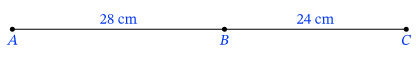
\includegraphics[width=0.7\textwidth]{Nagwa_Q1_D.png}
\end{figure}
%
\begin{multicols}{2}
\begin{itemize}
    \item[A.] $s=\cmcgs{28}$, $d=\cmcgs{28}$.
    \item[B.] $s=\cmcgs{76}$, $d=\cmcgs{76}$.
    \item[C.] $s=\cmcgs{52}$, $d=\cmcgs{28}$.
    \item[D.] $s=\cmcgs{76}$, $d=\cmcgs{28}$.
\end{itemize}
\end{multicols}
%
% \begin{solution}
% {\bf Distance Calculation:}\\
% The distance is the length over the path. The path is made up the following segments:
% \begin{equation*}
%     \text{Path}=\overline{AB}+\overline{BC}+\overline{CB}
% \end{equation*}
% The length of the segments is:
% \begin{equation*}
%     \begin{split}
%     & \overline{AB}=\cmcgs{28}\\
%     & \overline{BC}=\cmcgs{24}\\
%     & \overline{CB}=\cmcgs{24}\\
%     \end{split}
% \end{equation*}
% therefore,
% \begin{equation*}
%     \boxed{\text{Distance}=\overline{AB}+\overline{BC}+\overline{CB}=\cmcgs{28}+\cmcgs{24}+\cmcgs{24}=\cmcgs{76}}
% \end{equation*}
% {\bf Magnitude of displacement:}\\
% Initial point: $A$.\\
% Final point: $B$.\\
% \begin{equation*}
%     \boxed{\text{Displacement}=\overline{AB}=\cmcgs{28}\text{ to the right}}
% \end{equation*}
% \end{solution}
%
































\item According to the figure~\ref{acc}, a body moved from $\bm A$ to $\bm B$ along the line segment $\bm {\overline{AB}}$, and then it moved to $\bm C$ along $\bm {\overline{BC}}$. Finally, it moved to $\bm D$ along $\bm {\overline{CD}}$ and stopped there.\\
Find the \textbf{distance} covered by the body $\bm s$, and the \textbf{magnitude} of its \textbf{displacement} $\bm d$. \cite{Nagwa} Q. 11 Lesson Worksheet: Position, Displacement, and Distance\\
\textcolor{gray}{Help: Pythagoras's theorem might be useful to find the magnitude of the displacement: $a^2=b^2+c^2$.}
%
\begin{figure}[H]
    \centering
    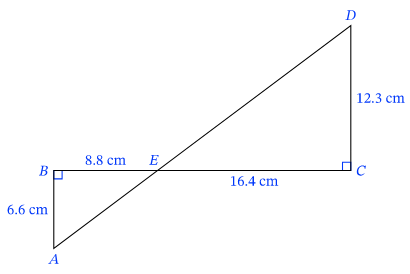
\includegraphics[width=0.7\textwidth]{Nagwa_Q11_D.png}
    \caption{}
    \label{acc}
\end{figure}
%
\begin{multicols}{2}
\begin{itemize}
    \item[A.] $s=\cmcgs{37.5}$, $d=\cmcgs{20.5}$.
    \item[B.] $s=\cmcgs{44.1}$, $d=\cmcgs{31.5}$.
    \item[C.] $s=\cmcgs{31.5}$, $d=\cmcgs{44.1}$.
    \item[D.] $s=\cmcgs{20.5}$, $d=\cmcgs{37.5}$.
\end{itemize}
\end{multicols}
%
\begin{example}
The initial point is: $A$.\\
The final point is: $D$.\\
The total distance is:
\begin{equation*}
    \text{Distance}=\overline{AB}+\overline{BC}+\overline{CD}
\end{equation*}
\begin{equation*}
    \boxed{\text{Distance}=\cmcgs{6.6}+\cmcgs{8.8}+\cmcgs{16.4}+\cmcgs{12.3}=\cmcgs{44.1}}
\end{equation*}
The magnitude of the displacement is just the length of the segment $\overline{AD}$. Using Pythagoras's theorem,
\begin{equation*}
    \boxed{\text{Magnitude of displacement}=\overline{AD}=\sqrt{(\overline{AB}+\overline{CD})^2+\overline{BC}^2}=\sqrt{\cmcgs{18.9^2}^2+\cmcgs{25.2^2}^2}=\cmcgs{31.5}}
\end{equation*}
\begin{equation*}
    \boxed{\text{The answer is:} \textbf{B. } \bm{s=\cmcgs{44.1}}\text{, }\bm{d=\cmcgs{31.5}}.}
\end{equation*}
\end{example}



















\item \label{Del} A delivery man has to deliver \textbf{5} parcels and go back to the headquarters office (\textbf{H}). The optimized order of the route is shown in the following figure. The sides of one square on the grid measure \textbf{250 m}. \cite{Triguero}
%
%
\begin{figure}[H]
\centering
\begin{tikzpicture}[on grid,scale = 0.67]
%------------------------------
% Un-comment for path ANSWER
%______________________________
 \draw[red,line width=1 mm] (-6,6)--(3,6)--(3,-6)--(7,-6)--(7,2)--(3.5,2);
\draw[red,line width=1 mm] (2.5,2)--(-3,2)--(-6,6);
%
\draw[blue,line width=1 mm,->] (-3.4,2)--(-5,4);
%
\draw[green,line width=1 mm,->] (-5.6,6)--(-4,4);
%
\draw[orange,line width=1 mm,->] (3,-5.6)--(6,-5.6);
%
%
%
%
%
%
%
    \foreach \i in {-8,...,8} {
        \draw [very thin,gray] (\i,-8) -- (\i,8);
    }
    \foreach \i in {-8,...,8} {
        \draw [very thin,gray] (-8,\i) -- (8,\i);
    }
    \draw[black,fill] (-6,6) circle [radius=0.45] node {\textcolor{white}{\bf H}};
    \draw[black,fill] (3,6) circle [radius=0.45] node {\textcolor{white}{\bf 1}};
    \draw[black,fill] (3,-6) circle [radius=0.45] node {\textcolor{white}{\bf 2}};
    \draw[black,fill] (7,-6) circle [radius=0.45] node {\textcolor{white}{\bf 3}};
    \draw[black,fill] (7,2) circle [radius=0.45] node {\textcolor{white}{\bf 4}};
    \draw[black,fill] (-3,2) circle [radius=0.45] node {\textcolor{white}{\bf 5}};
\end{tikzpicture}
\end{figure}
%
\begin{itemize}
    \item[\bf (a)] \textbf{Draw} the path. The circled numbers indicate the position and order of the different deliver stops on the route.
    \item[\bf (b)] Calculate the \textbf{total} \textbf{distance} gone by the delivery man (from \textbf{H} to \textbf{H} passing through all the deliver stops).
    %What is the total distance of the delivery path (from H to H)?
    %
    % \begin{solution}
    % Let's count all squares along the path. 1 square = the length of the side:
    %  \begin{equation*}
    % \begin{split}
    % & s_\text{H-1}=9\text{ square}\\
    % & s_\text{1-2}=12\text{ square}\\
    % & s_\text{2-3}=4\text{ square}\\
    % & s_\text{3-4}=8\text{ square}\\
    % & s_\text{4-5}=10\text{ square}\\
    % & s_\text{5-H}=\sqrt{3^2+4^2}\text{ square}=\sqrt{25}\text{ square}=5\text{ square}\\
    % \end{split}
    % \end{equation*}
    % every square (side of the square) is equivalent to 250 m, therefore,
    % \begin{equation*}
    % \boxed{
    %     \text{Total distance}=48\text{ square}\cdot 250\text{ m/square}=\msis{12000}=\km{12}}
    % \end{equation*}
    % \end{solution}
    % 
    % 
    %
    %
    \item[\bf (c)] What is the \textbf{displacement} of the trip from \textbf{H} to \textbf{5}? (give the magnitude of the displacement (use Pythagoras theorem) and draw an arrow for the direction)
    %
    % \begin{solution}
    % \begin{equation*}
    %     \boxed{\text{Magnitude of the displacement 5$-$H}=d_{5-\text{H}}\cdot\msis{250}/\text{square}=\msis{1250}}
    % \end{equation*}
    % The direction has been represented in blue on the grid.
    % \end{solution}
    %
    \item[\bf (d)] What is the \textbf{displacement} of the trip from \textbf{5} to \textbf{H}? (give the magnitude of the displacement (use Pythagoras theorem) and draw an arrow for the direction)
     %
    % \begin{solution}
    % \begin{equation*}
    %     \boxed{\text{Magnitude of the displacement H$-$5}=d_{5-\text{H}}\cdot\msis{250}/\text{square}=\msis{1250}}
    % \end{equation*}
    % The direction has been represented in green on the grid.
    % \end{solution}
    %
    \item[\bf (e)] What is the \textbf{distance} of the trip from \textbf{2} to \textbf{4}?
    %
    % \begin{solution}
    % \begin{equation*}
    %     \boxed{\text{distance }2-4=s_{2-3}+s_{3-4}=4\text{ squares}\cdot\msis{250}/\text{square}+8\text{ squares}\cdot\msis{250}/\text{square}=\km{3}} 
    % \end{equation*}
    % \end{solution}
    %
    \item[\bf (f)] What is the \textbf{distance} of the trip from \textbf{2} to \textbf{3}?
    %
    % \begin{solution}
    % \begin{equation*}
    %     \boxed{\text{distance }2-3=s_{2-3}=4\text{ squares}\cdot\msis{250}/\text{square}=\km{1}} 
    % \end{equation*}
    % \end{solution}
    %
    \item[\bf (g)] What is the \textbf{displacement} of the trip from \textbf{2} to \textbf{3}? (give the magnitude of the displacement and draw an arrow for the direction)
    %
    % \begin{solution}
    % \begin{equation*}
    %     \boxed{\text{distance }2-3=s_{2-3}=4\text{ squares}\cdot\msis{250}/\text{square}=\km{1}} 
    % \end{equation*}
    % The direction is indicated in the graph in orange color.
    % \end{solution}
    %
    \item[\bf (h)] Calculate the \textbf{total} \textbf{displacement} gone by the delivery man (from \textbf{H} to \textbf{H} passing through all the deliver stops).
    % \begin{solution}
    % The total displacement is composed by the distance from the initial and final point, and the direction. The total distance from the initial point to the final point is \textbf{zero}. The initial and final point is the same.
    % \begin{equation*}
    %     \boxed{\text{Displacement}=0 \text{. No direction associated to zero.}}
    % \end{equation*}
    % \end{solution}
\end{itemize}













% \item \textbf{Explain} the difference between: \cite{CCEADA} p. 347 show you can
% \begin{itemize}
%     \item[\bf (a)] \textbf{Distance} and \textbf{displacement}.
%     %
%     % \begin{solution}
%     % Distance is a scalar, a positive number. Displacement is a vector. Distance is the \textbf{length} of space between two points over a \textbf{given path}. Displacement is the \textbf{length} of space \textbf{and} \textbf{direction} between a reference and a point over the \textbf{shortest} path.
%     % \end{solution}
%     %
%     \item[\bf (b)] \textbf{Speed} and \textbf{velocity}.
%     %
%     % \begin{solution}
%     % Speed is a scalar, a positive number. Velocity is a vector. The speed is the rate of change of the distance with respect to time while velocity is the rate of change of displacement with respect to time.
%     % \end{solution}
%     %
% \end{itemize}











% \item Classify the following quantities in the following two categories: Scalar or vector. \textcolor{gray}{\bf [SPEC M6]} \cite{Triguero}\\

% \begin{table}[H]
%     \centering
%     \scalebox{1.5}{
%     \begin{tabular}{|l|c|c|}\hline
%     \rowcolor{yellow}{\bf Quantity name & \bf Scalar/Vector & \bf Units}\\\hline
%     velocity    & \textcolor{white}{Vector} & \textcolor{white}{m/s} \\\hline
%     time        & \textcolor{white}{Scalar} & \textcolor{white}{s} \\\hline
%     distance    & \textcolor{white}{Scalar} & \textcolor{white}{m} \\\hline
%     displacement    & \textcolor{white}{Vector} & \textcolor{white}{m} \\\hline
%     rate of change of speed  & \textcolor{white}{Scalar}  & \textcolor{white}{m/s$^2$} \\\hline
%     acceleration      &  \textcolor{white}{Vector} & \textcolor{white}{m/s$^2$} \\\hline
%     average velocity      & \textcolor{white}{Vector} & \textcolor{white}{m/s} \\\hline
%     average speed   & \textcolor{white}{Scalar} & \textcolor{white}{m/s} \\\hline
%     average rate of change of speed & \textcolor{white}{-} & \textcolor{white}{-}\\\hline
%     \end{tabular}}
% \end{table}
% %
% %
% %
% %
% %
% %
% %
% %
% %
% %
% %
% %
% %
% %
% %
% %
% %
% %
% %
% %
% \item Copy and complete the following Table~\ref{ddd}.  \cite{CCEADA} p. 354 TY. 8  \textcolor{gray}{\bf [SPEC M6]} 
% %
% \begin{table}[H]
%     \centering
%     \scalebox{1.3}{
%     \begin{tabular}{|l|l|c|}\hline
%     \rowcolor{yellow}{\bf Name of quantity & \bf Definition & \bf Scalar or vector}\\\hline
%     \bf Distance & \textcolor{white}{Length of the space between} & Scalar\\
%     & \textcolor{white}{two points over a given path.} & \\\hline
%     \bf Displacement & \textcolor{white}{Length of the space and direc}  & \textcolor{white}{Vector}\\
%     & \textcolor{white}{tion from a reference to a point.} & \\\hline
%     \bf Speed & Rate of change of distance  & Scalar\\
%       & with respect to time.  & \\\hline
%     \bf Velocity & \textcolor{white}{Rate of change of displacement}  &  vector\\
%     & \textcolor{white}{with respect to time} & \\\hline
%     \bf Acceleration & Rate of change of velocity  & \textcolor{white}{Vector}\\
%       & with respect to time  & \\\hline
%     \end{tabular}}
%     \caption{}
%     \label{ddd}
% \end{table}
% %
% %
% %
% %
% %
% %
% %
% %
% %
% %
% %
% %
% %
% \item Pearl climbs to the top of a slide. CCEA MAY 2019
% %
% \begin{figure}[H]
%     \centering
%     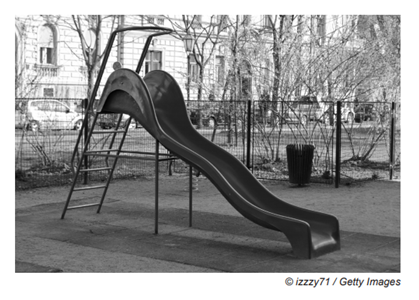
\includegraphics[width=0.7\textwidth]{prob7.png}
%     \caption{}
%     \label{fig:my_label}
% \end{figure}
% %
% \begin{itemize}
%     \item[\bf (a)] Pearl has \textbf{speed}, \textbf{velocity} and \textbf{acceleration} as she slides down. \textbf{Complete} the table \ref{rakas} to indicate whether these quantities are \textbf{scalars} or \textbf{vectors}. In each case indicate your choice with a tick ($\checkmark$).
% %
% \begin{table}[H]
%     \centering
%     \scalebox{1.5}{
%     \begin{tabular}{|l|c|c|}
%     \cline{2-3}
%      \multicolumn{1}{c |}{} & \cellcolor{yellow} \textbf{Scalar} & \cellcolor{yellow} \textbf{Vector} \\\hline
%     \cellcolor{yellow} \textbf{Speed}        &  \textcolor{white}{$\checkmark$} &      \\\hline
%     \cellcolor{yellow} \textbf{Velocity}    &        & \textcolor{white}{$\checkmark$} \\\hline
%     \cellcolor{yellow} \textbf{Acceleration} &        & \textcolor{white}{$\checkmark$} \\\hline
%      \cellcolor{yellow} \textbf{time} & \textcolor{white}{$\checkmark$}  &  \\\hline
%     \end{tabular}}
%     \caption{}
%     \label{rakas}
% \end{table}
% %
% \item[\bf (b)] Study the shape of the slide in the diagram. Consider Pearl’s displacement and distance from the top to the bottom. Choose the correct statement below (Table \ref{crocos}) by ticking ($\checkmark$) the box.
% \begin{table}[H]
%     \centering
%     \scalebox{1.5}{
%     \begin{tabular}{|l|c|}\hline
%   Her displacement and distance are equal.     & \\\hline
%   Her displacement is greater than her distance.     & \\\hline
%   Her distance is greater than her displacement.    & \textcolor{white}{$\checkmark$} \\\hline
%     \end{tabular}}
%     \caption{}
%     \label{crocos}
% \end{table}
% \end{itemize}




























\section*{\textcolor{red}{Distance-time and Displacement-time graphs: Speed \& Velocity}}

%
% ADD \href{https://www.nagwa.com/en/worksheets/494103929802/}{Lesson Worksheet: Calculating Speed from Distance–Time Graphs}
%


\subsection*{\textcolor{red}{\underline{Basics:}}}
% FALTA 10 y 7




\item The graph of distance and time shows a set of points. \textbf{Which} of the following does each marker on the graph show? \cite{Nagwa} Q. 6 \href{https://www.nagwa.com/en/worksheets/964158724874/}{Lesson Worksheet: Distance–Time Graphs}
%
\begin{figure}[H]
    \centering
    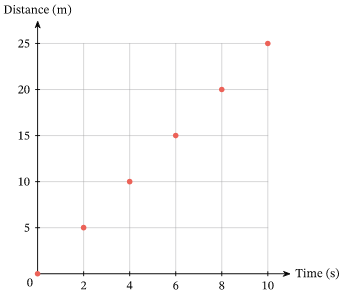
\includegraphics{Nagwa_Q6_kin.png}
    % \caption{}
    % \label{fig:my_label}
\end{figure}
%
\begin{itemize}
    \item[A.] A value of \textbf{time} only.
    \item[B.] A value of \textbf{distance} only.
    \item[C.] A value of \textbf{distance} and a value of \textbf{time}.
    %
    % Answer
    %
    %\item[\textcolor{blue}{\bf C.}] \textcolor{blue}{\bf A value of \textbf{distance} and a value of \textbf{time}.}
\end{itemize}








\item The table shows five readings of the distance traveled by a toy car that moved for \textbf{10 seconds}. The \textbf{distance} was measured at \textbf{2 s intervals}. \textbf{Which} color \textbf{axis} of the graph must \textbf{show} the \textbf{time} that the car moves for? \cite{Nagwa} Q. 9 \href{https://www.nagwa.com/en/worksheets/932192593730/}{Lesson Worksheet: Distance–Time Graphs}
%
\begin{figure}[H]
    \centering
    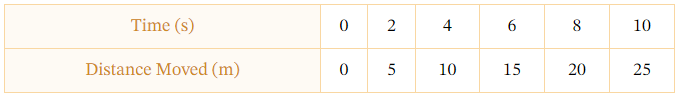
\includegraphics[width=0.7\textwidth]{Nagwa_Q9_kin-1.png}
    % \caption{}
    % \label{fig:my_label}
\end{figure}
%
\begin{figure}[H]
    \centering
    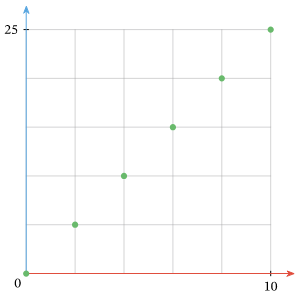
\includegraphics{Nagwa_Q9_kin-2.png}
    % \caption{}
    % \label{fig:my_label}
\end{figure}
%
\begin{multicols}{2}
\begin{itemize}
    \item[A.] Red
    %
    % Answer
    %
    %\item[\textcolor{blue}{\bf A.}] \textcolor{blue}{\bf Red}}
    \item[B.] Blue
\end{itemize}
\end{multicols}


















\item A toy car is made to travel different \textbf{distances}, and the \textbf{time taken} to travel each distance is \textbf{recorded}. The results are shown in the table and also on the graph. \textbf{Which reading} from the \textbf{table} records the measurement of distance and time that are shown by the \textbf{pink marker} on the graph? \cite{Nagwa} Q. 8 \href{https://www.nagwa.com/en/worksheets/932192593730/}{Lesson Worksheet: Distance–Time Graphs}
%
\begin{figure}[H]
    \centering
    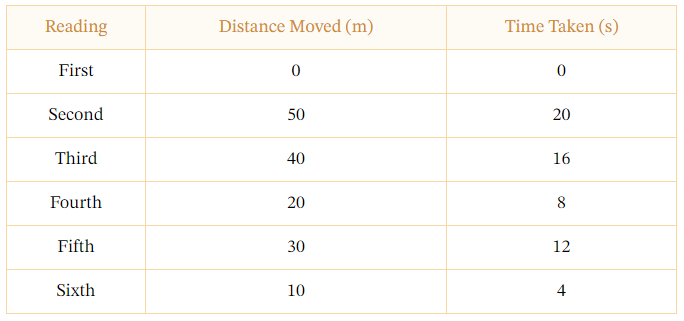
\includegraphics[width=0.7\textwidth]{Nagwa_Q8_kin-1.png}
    % \caption{}
    % \label{fig:my_label}
\end{figure}
%
\begin{figure}[H]
    \centering
    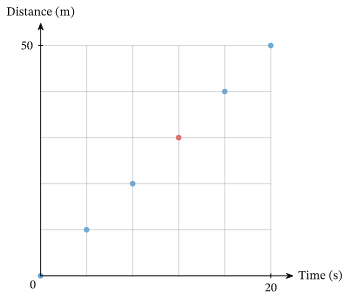
\includegraphics{Nagwa_Q8_kin-2.png}
    % \caption{}
    % \label{fig:my_label}
\end{figure}
%
\begin{itemize}
    \item[A.] Fourth
    \item[B.] Fifth
    %
    % Answer
    %
    %\item[\textcolor{blue}{\bf B.}] \textcolor{blue}{\bf Fifth}}
    \item[C.] Third
\end{itemize}
%
% \begin{solution}
% * Every tick on the horizontal axis represents 4 seconds. The time for the pink point is,
% \begin{equation*}
%     3\text{ ticks}\cdot \tsis{4}=\tsis{12}
% \end{equation*}
% * Every tick on the vertical axis represents 10 metres. The distance for the pink point is,
% \begin{equation*}
%     3\text{ ticks}\cdot \msis{10}=\tsis{30}
% \end{equation*}
% \end{solution}














\item \textbf{Which} of the following \textbf{graphs} correctly shows the \textbf{distances} and \textbf{times} in the \textbf{table}? \cite{Nagwa} Q. 2 \href{https://www.nagwa.com/en/worksheets/932192593730/}{Lesson Worksheet: Distance–Time Graphs}\\
%
\begin{figure}[H]
    \centering
    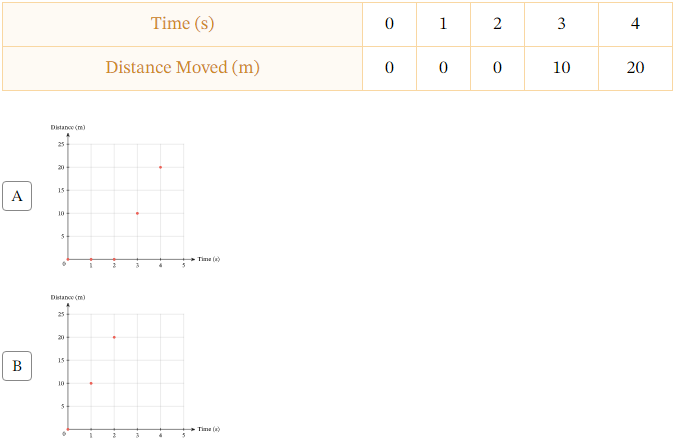
\includegraphics[width=0.7\textwidth]{Nagwa_Q2_kin.png}
    % \caption{}
    % \label{fig:my_label}
\end{figure}
%
% \begin{solution}
% \begin{equation*}
%     \text{The answer is graph \textbf{A}}
% \end{equation*}
% The seconds 0, 1 and 2 the table shows that the distance is NOT changing. After second 2 the distance changes. This is only compatible with graph A.
% \end{solution}
















\item The graph shows the \textbf{distance} three toy cars \textbf{move each second}. \textbf{Which} of the \textbf{tables} shows the motion of the car represented by the \textbf{orange} crosses on the graph? \cite{Nagwa} Q. 4 \href{https://www.nagwa.com/en/worksheets/932192593730/}{Lesson Worksheet: Distance–Time Graphs}\\
%
\begin{figure}[H]
    \centering
    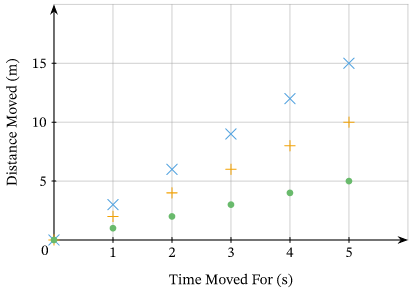
\includegraphics[width=0.7\textwidth]{Nagwa_Q4_kin.png}
    % \caption{}
    % \label{fig:my_label}
\end{figure}
%
%
\begin{figure}[H]
    \centering
    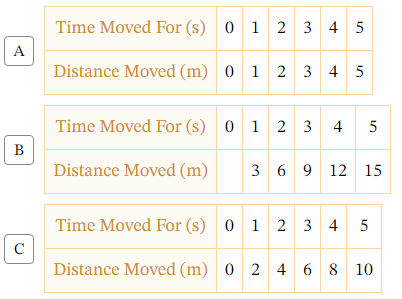
\includegraphics{Nagwa_Q4_kin-2.png}
    % \caption{}
    % \label{fig:my_label}
\end{figure}
%
% \begin{solution}
% \begin{equation*}
%     \boxed{\text{The answer is graph \textbf{C}}}
% \end{equation*}
% We can take specific points for the graph with crosses, for example the point,\\

% time $=$ 5 seconds\\
% and\\
% distance $=$ 10 metres. 

% This point can be only found in table \textbf{C}.
% \end{solution}






\subsection*{\textcolor{red}{\underline{Speed}}}








\item Fill in the blank: \cite{Nagwa} Q. 3 \href{https://www.nagwa.com/en/worksheets/964158724874/}{Lesson Worksheet: Distance–Time Graphs}\\ 
On a \textbf{distance-time} graph, the \textbf{less steep} the line through a set of points, the \underline{\hspace{3cm}} meters move in one second.
%
\begin{multicols}{2}
\begin{itemize}
    \item[A.] Fewer
    %\item[\textcolor{blue}{ \textbf{A.}}] \textcolor{blue}{ \textbf{Fewer}}
    \item[B.] More
\end{itemize}
\end{multicols}








\item Fill in the blank: \cite{Nagwa} Q. 5 \href{https://www.nagwa.com/en/worksheets/964158724874/}{Lesson Worksheet: Distance–Time Graphs}\\ 
On a \textbf{distance–time} graph, the \textbf{steeper} the line through a set of points, the \underline{\hspace{3cm}} the time taken to move one meter.
%
\begin{multicols}{2}
\begin{itemize}
    \item[A.] More
    \item[B.] Less
    %\item[\textcolor{blue}{ \textbf{B.}}] \textcolor{blue}{ \textbf{Less}}
\end{itemize}
\end{multicols}










\item \textbf{Which} of the following \textbf{quantities} is equal to the \textbf{gradient} of the type of graph shown? \cite{Nagwa} Q. 7 Lesson Worksheet: Kinematic Graphs

\begin{figure}[H]
    \centering
    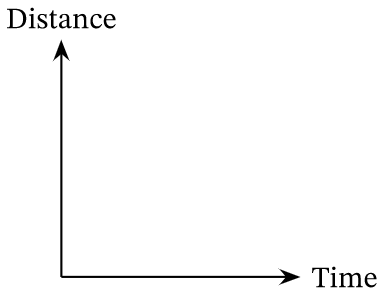
\includegraphics{triguijoc.png}
    \caption{}
    \label{fig:my_label}
\end{figure}

\begin{itemize}
    \item[A.] Acceleration
    \item[B.] Change in velocity
    \item[C.] Speed
    %\item[\textcolor{blue}{\bf C.}] \textcolor{blue}{\bf Speed}
    \item[D.] Velocity
    \item[E.] Displacement
\end{itemize}












\item \textbf{Which} color line on the graph shows the \textbf{greatest speed}? \cite{Nagwa} Q. 1 \href{https://www.nagwa.com/en/worksheets/964158724874/}{Lesson Worksheet: Distance–Time Graphs}
%
\begin{figure}[H]
    \centering
    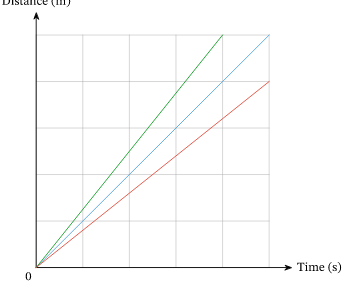
\includegraphics{Nagwa_Q1_kin.png}
    \caption{}
    \label{fig:my_label}
\end{figure}
%
\begin{multicols}{3}
\begin{itemize}
    \item[A.] Red
    \item[B.] Blue
    \item[C.] Green
    %\item[\textcolor{blue}{\bf C.}] \textcolor{blue}{\bf Green}
\end{itemize}
\end{multicols}












%\href{https://www.nagwa.com/en/worksheets/184171967276/}{Lesson Worksheet: Displacement–Time Graphs}\\




























\item For times \textbf{after} the first \textbf{four seconds} shown on the graph, \textbf{which color} line shows the \textbf{greatest speed}? \cite{Nagwa} Q. 7 \href{https://www.nagwa.com/en/worksheets/964158724874/}{Lesson Worksheet: Distance–Time Graphs}
%
\begin{figure}[H]
    \centering
    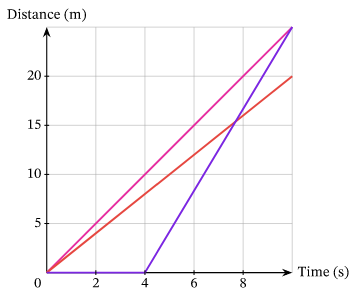
\includegraphics[scale=0.7]{Nagwa_Q7_kin.png}
    \caption{}
    \label{fig:my_label}
\end{figure}
%
\begin{multicols}{3}
\begin{itemize}
    \item[A.] Pink
    %
    \item[B.] Purple
    %\item[\textcolor{blue}{\bf B.}] \textcolor{blue}{\bf Purple}
    \item[C.] Red
\end{itemize}
\end{multicols}














\item The motion of a running man is shown by the \textbf{blue line}. The \textbf{red line} shows the motion of a woman who is also running. \textbf{Which} of the following is \textbf{correct}? \cite{Nagwa} Q. 10 \href{https://www.nagwa.com/en/worksheets/964158724874/}{Lesson Worksheet: Distance–Time Graphs}
%
\begin{figure}[H]
    \centering
    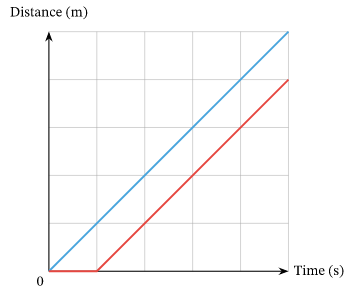
\includegraphics[scale=0.7]{Nagwa_Q10_kin.png}
    \caption{}
    \label{fig:my_label}
\end{figure}
%
\begin{itemize}
    \item[A.] The \textbf{woman} started to run \textbf{before} the man did.
    \item[B.] Both the \textbf{man} and the \textbf{woman} started to run at the \textbf{same time}.
    \item[C.] The \textbf{woman} started to run \textbf{after} the man did.
    %\item[\textcolor{blue}{\bf C.}] \textcolor{blue}{\bf The woman started to run after the man did.}
\end{itemize}












\item A student records the \textbf{distance} travelled with his bike at different times and obtains the following data. \cite{Triguero}
%
\begin{table}[H]
    \centering
    \scalebox{1.25}{
    \begin{tabular}{|c|c|}\hline
    \rowcolor{yellow}{\bf time/s  & \bf Position/m}  \\\hline
    0       & 0 \\\hline
    1       & 5 \\\hline
    3       & 15 \\\hline
    4       & 20 \\\hline
    6       & 30 \\\hline
    \end{tabular}}
    \caption{Bike's position at different times.}
    \label{chakiteki}
\end{table}
%
\begin{itemize}
    \item[\bf (a)] Represent the \textbf{displacement-time graph}.
    %
    \begin{example}
\begin{figure}[H]
    \centering
  \begin{tikzpicture}
	\begin{axis}[
		height=10cm,
		width=16cm,
		grid=major,xlabel={\Large time, $t$[s]},ylabel={\Large distance, $d$[m]},enlargelimits=false
	]

%%%%%%%%%%%%%blue/white 
	\addplot[Greenss,mark=*,mark size=1mm] coordinates {
		(0,0)
		(1,5)
		(3,15)
		(4,20)
		(6,30)
	};
	\end{axis}
    \end{tikzpicture}
    \caption{Distance-time graph.}
    \label{fig:my_label}
    \end{figure}
    \end{example}
    %
    \item[\bf (b)] At what \textbf{distance} is the student after \textbf{2 seconds}.
    %
    \begin{example}
    Looking at the graph one can easily infer, that at time \textbf{2 seconds} (horizontal axis), the distance is \textbf{10 metres}. % (see red lines on the graph).
    \begin{equation*}
        \boxed{\text{Distance at 2 seconds}=\msis{10}}
    \end{equation*}
    \end{example}
    %
    \item[\bf (c)] At what \textbf{time} the student was at a distance of \textbf{25 metres}.
    %
    \begin{example}
    Looking at the graph one can easily infer, that at distance \textbf{25 metres} (vertical axis), the time is \textbf{5 seconds}.% (see red lines on the graph).
    \begin{equation*}
        \boxed{\text{Time at 25 metres}=\tsis{5}}
    \end{equation*}
    \end{example}
    %
    \item[\bf (d)] Calculate the \textbf{average speed} between the \textbf{initial} time and the \textbf{final} time shown in the table~\ref{chakiteki}.
    %
    \begin{example}
    The \textbf{average speed} is the \textbf{gradient} (also called slope) of the line \textbf{connecting} the \textbf{``initial"} and \textbf{``final"} points on the distance-time graph. Speed can be understood as the rate of change of distance with respect to time.
    \begin{equation*}
        \begin{split}
            &\text{Initial point}=(\tsis{0},\msis{0})\\
            &\text{Final point}=(\tsis{6},\msis{30})\\
        \end{split}
    \end{equation*}
    \begin{equation*}
    \boxed{\text{Speed}=\frac{\text{distance}}{\text{time}}=\frac{\msis{30}-\msis{0}}{\tsis{6}-\tsis{0}}=\frac{\msis{30}}{\tsis{6}}=\vsis{5}}
    \end{equation*}
    \end{example}
    %
\end{itemize}

















\item Paul and Jim set off at the \textbf{same time from their separate houses} to travel to a nearby shop. Table~\ref{paulini} shows the \textbf{distances travelled by Paul to the shop}. \cite{CCEADA,Triguero} p. 355 pb. 1
%
\begin{table}[H]
    \centering
    \scalebox{1.3}{
    \begin{tabular}{|l|l|c|c|c|c|c|c|c|}\hline
    \cellcolor{yellow}{\bf Distance Travelled by Paul [m]} & 0 & 3 & 6 & 9 & 12 & 15 & 18 & 21\\\hline
    \cellcolor{yellow}{\bf Time elapsed [s]} & 0 & 1 & 2 & 3 & 4 & 5 & 6 & 7\\\hline
    \end{tabular}}
    \caption{}
    \label{paulini}
\end{table}
%
\begin{itemize}
    \item[\bf (a)] Draw a graph of \textbf{distance against time} for Paul's journey.
    %
%
\end{itemize}
Table~\ref{kJimx} shows the \textbf{distances travelled by Jim} to the same shop.
%
\begin{table}[H]
    \centering
    \scalebox{1.3}{
    \begin{tabular}{|l|l|c|c|c|c|c|c|c|}\hline
    \cellcolor{yellow}{\bf Distance Travelled by Jim} & 0 & 2 & 4 & 6 & 8 & 10 & 12 & 14\\\hline
    \cellcolor{yellow}{\bf Time elapsed} & 0 & 1 & 2 & 3 & 4 & 5 & 6 & 7\\\hline
    \end{tabular}}
    \caption{}
    \label{kJimx}
\end{table}
%
\begin{itemize}
    \item[\bf (b)] Draw a graph of \textbf{distance against time} for Jim's journey \textbf{on the same axes}.
    %
    %
    %
    %
    % ANSWER GRAPH!
    %
    %
    %
    %
\begin{figure}[H]
    \centering
  \begin{tikzpicture}
	\begin{axis}[enlargelimits=false,
		height=12cm,
		width=16cm,
		grid=major,xlabel={\Large time, $t$[s]},ylabel={\Large distance, $d$[m]},legend style={at={(axis cs:1,15)},anchor=north},clip=false
	]%red/white
	\addplot[red,line width=0.5mm,mark=*] coordinates {
		(0,0)
		(1,3)
		(2,6)
		(3,9)
		(4,12)
		(5,15)
		(6,18)
		(7,21)
	};
 	\addlegendentry{Paul}
 	%blue/white
 	\addplot[blue,line width=0.5mm,mark=+] coordinates {
		(0,0)
		(1,2)
		(2,4)
		(3,6)
		(4,8)
		(5,10)
		(6,12)
		(7,14)
	};
 	\addlegendentry{Jim}
 	\node at (axis cs:-0.6,0) {Home};
 	\node at (axis cs:-0.15,11) {\bf 11};
 	\node at (axis cs:7,-2) {Shop};
 	%
 	%
 	% BEGIN ANSWER
 	%
 	%
%  	\draw[dashed,line width=0.25mm] (axis cs:0,11)--(axis cs:3.67,11);
%  	\draw[dashed,line width=0.25mm] (axis cs:3.67,11)--(axis cs:3.67,0);
%  	%
%  	\draw[dashed,line width=0.25mm] (axis cs:0,11)--(axis cs:5.5,11);
%  	\draw[dashed,line width=0.25mm] (axis cs:5.5,11)--(axis cs:5.5,0);
%  	%
%  	\draw[line width=0.5mm,<->] (axis cs:0,11.2)--(axis cs:3.67,11.2);
%  	%
%  	\draw[line width=0.5mm,<->] (axis cs:0,10.8)--(axis cs:5.5,10.8);
%  	%
%  	\draw[dashed,line width=0.25mm] (axis cs:2.5,0)--(axis cs:2.5,7.5);
%  	\draw[line width=0.5mm,<->] (axis cs:2.5,5)--(axis cs:2.5,7.5);
%  	\draw[line width=0.25mm,dashed] (axis cs:0,7.5)--(axis cs:2.5,7.5);
%  	\draw[line width=0.25mm,dashed] (axis cs:0,5)--(axis cs:2.5,5);
	%
 	%
 	% END ANSWER
 	%
 	%
	\end{axis}

\end{tikzpicture}
    \caption{Distance-time graphs for Paul and Jim.}
\end{figure}
    %
    %
    %
    %
    %
    %
    %
    %
    %
    %
    %
    %
    %
    %
    %
    \item[\bf (c)] Use the graphs to answer the following questions.
    \begin{itemize}
        \item[\bf (i)] Which person is going \textbf{faster}?
        %
        % \begin{solution}
        % {\bf Graphical Answer:}\\
        % The speed for each person is the slope of the graph. Paul's slope is larger than Jim's slope. This means that Paul's speed is larger.
        % \begin{equation*}
        % \boxed{
        %     \text{\bf Paul is going faster}}
        % \end{equation*}
        % \\
        % {\bf Calculated Answer:}\\
        % It is \textbf{NOT} needed in this section but we can calculate the speeds and compare:
        % \begin{equation*}
        %     \text{Speed Paul}=\frac{\text{distance}}{\text{time}}=v=\frac{d}{t}=\frac{\msis{21}}{\tsis{7}}=\vsis{3}
        % \end{equation*}
        % \begin{equation*}
        %     \text{Speed Jim}=\frac{\text{distance}}{\text{time}}=v=\frac{d}{t}=\frac{\msis{14}}{\tsis{7}}=\vsis{2}
        % \end{equation*}
        % therefore we can state that Paul is going faster.
        % \end{solution}
        %
        %
        \item[\bf (ii)] \textbf{How long} does it take Paul and Jim to travel \textbf{11 m}?
        %
        % \begin{solution}
        % {\bf Graphical Answer:}\\
        % Go to graph!
        % \\
        % {\bf Calculated Answer:}\\
        % \begin{equation*}
        %     \text{Speed Jim}=\frac{\text{distance}}{\text{time}}\Longrightarrow \boxed{\text{time Jim}=\frac{\text{distance}}{\text{speed}}=\frac{d}{v}=\frac{\msis{11}}{\vsis{3}}=\tsis{3.67}}
        % \end{equation*}
        % \begin{equation*}
        %     \text{Speed Paul}=\frac{\text{distance}}{\text{time}}\Longrightarrow \boxed{\text{time Paul}=\frac{\text{distance}}{\text{speed}}=\frac{d}{v}=\frac{\msis{11}}{\vsis{2}}=\tsis{5.5}}
        % \end{equation*}
        % \end{solution}
        %
        %
        \item[\bf (iii)] How \textbf{far apart} are Paul and Jim after \textbf{2.5 s}?
        %
        % \begin{solution}
        % {\bf Graphical Answer:}\\
        % Go to graph!
        % \\
        % {\bf Calculated Answer:}\\
        % The distance between Paul and Jim at $t=2.5$ s is the distance of Paul  at $t=2.5$ s minus the distance of Jim at $t=2.5$ s.
        % \begin{equation*}
        %     \text{Speed Paul}=\frac{\text{distance}}{\text{time}}\Longrightarrow \boxed{\text{distance Paul}=\text{speed}\times\text{time}=\vsis{3}\times\tsis{2.5}=\msis{7.5}}
        % \end{equation*}
        % \begin{equation*}
        %     \text{Speed Jim}=\frac{\text{distance}}{\text{time}}\Longrightarrow \boxed{\text{distance Jim}=\text{speed}\times\text{time}=\vsis{2}\times\tsis{2.5}=\msis{5}}
        % \end{equation*}
        % therefore,
        % \begin{equation*}
        %  \boxed{\text{distance between  Jim and Paul}=\msis{7.5}-\msis{5}=\msis{2.5}}
        % \end{equation*}
        % \end{solution}
        %
        \item[\bf (iv)] Is Paul's \textbf{speed steady}?
        %
        % \begin{solution}
        % Yes. The slope of the graph does not change (the speed of the movement does not change).
        % \end{solution}
        %
        \item[\bf (vi)] What is Jim's \textbf{average speed}?
        %
        % \begin{solution}
        % \begin{equation*}
        %     \text{Speed Jim}=\frac{\text{distance}}{\text{time}}=v=\frac{d}{t}=\frac{\msis{14}}{\tsis{7}}=\vsis{2}
        % \end{equation*}
        % \begin{equation*}
        % \boxed{
        %     \text{\bf Jim average speed is } \vsis{2}}
        % \end{equation*}
        % \end{solution}
        %
        \item[\bf (vii)] Who lives \textbf{closer} to the shop?
        %
        % \begin{solution}
        % \begin{equation*}
        % \boxed{
        %     \text{\bf Jim lives closer to the shop}}
        % \end{equation*}
        % Jim lives at 14 m while Paul lives at 21 m.
        % \end{solution}
        %
    \end{itemize}
\end{itemize}














% Move this before paul and jim
\item The graph shows the \textbf{distance} covered in kilometers over a 15-hour hike. What were the \textbf{fastest} and \textbf{slowest} \textbf{speeds} recorded? \cite{Nagwa} Q. 1 \href{https://www.nagwa.com/en/worksheets/932192593730/}{Lesson Worksheet: Distance-Time Graphs}
%
\begin{figure}[H]
    \centering
    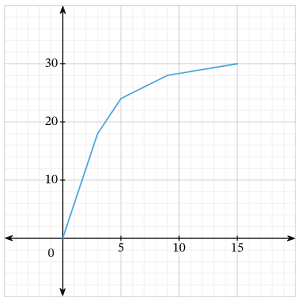
\includegraphics[scale=1]{Nagwa_Q1_kin2.png}
\end{figure}
%
\begin{itemize}
    \item[A. ] \textbf{fastest speed:} $-6$ km/h, \textbf{slowest speed:} $-1/3$ km/h.
    \item[B. ] \textbf{fastest speed:} $6$ km/h, \textbf{slowest speed:} $-1/3$ km/h.
    \item[C. ] \textbf{fastest speed:} $3$ km/h, \textbf{slowest speed:} $1/3$ km/h.
    \item[D. ] \textbf{fastest speed:} $6$ km/h, \textbf{slowest speed:} $1/3$ km/h.
    \item[E. ] \textbf{fastest speed:} $3$ km/h, \textbf{slowest speed:} $1/6$ km/h.
\end{itemize}
%
% \begin{solution}
% We can clearly identify on the graph 4 different slopes i.e. 4 different speeds. Let us calculate the slopes.
% \begin{equation*}
%     \text{Slope}=\frac{\text{Rise $y$ axis}}{\text{Run $x$ axis}}
% \end{equation*}
% \textbf{\underline{From 0 to 3 hours the speed was:}}
% \begin{equation*}
%     \text{Speed}=\text{Slope}=\frac{\text{Rise $y$ axis}}{\text{Run $x$ axis}}=\frac{\km{18}-\km{0}}{\hours{3}-\hours{0}}=\frac{\km{18}}{\hours{3}}=\kmh{6}
% \end{equation*}
% \textbf{\underline{From 3 to 5 hours the speed was:}}
% \begin{equation*}
%     \text{Speed}=\text{Slope}=\frac{\text{Rise $y$ axis}}{\text{Run $x$ axis}}=\frac{\km{24}-\km{18}}{\hours{5}-\hours{3}}=\frac{\km{6}}{\hours{2}}=\kmh{3}
% \end{equation*}
% \textbf{\underline{From 5 to 9 hours the speed was:}}
% \begin{equation*}
%     \text{Speed}=\text{Slope}=\frac{\text{Rise $y$ axis}}{\text{Run $x$ axis}}=\frac{\km{28}-\km{24}}{\hours{9}-\hours{5}}=\frac{\km{4}}{\hours{4}}=\kmh{1}
% \end{equation*}
% \textbf{\underline{From 9 to 15 hours the speed was:}}
% \begin{equation*}
%     \text{Speed}=\text{Slope}=\frac{\text{Rise $y$ axis}}{\text{Run $x$ axis}}=\frac{\km{30}-\km{28}}{\hours{15}-\hours{9}}=\frac{\km{2}}{\hours{6}}=\kmh{1/3}
% \end{equation*}
% The \textbf{speed} is always \textbf{positive} because the \textbf{distance} is always \textbf{positive}. All negative number answers are incorrect.

% From the above calculations of the speed,

% \begin{equation*}
%     \text{Fastest speed}=\kmh{6}
% \end{equation*}

% \begin{equation*}
%     \text{Slowest speed}=\kmh{1/3}
% \end{equation*}

% \begin{equation*}
%     \boxed{\text{\bf{The answer is D}}\\
%     \textbf{fastest speed:} $6$ km/h, \textbf{slowest speed:} $1/3$ km/h.}
% \end{equation*}

% \end{solution}
%








% Move this before paul and jim
\item \textcolor{red}{ERASE} The following displacement-time graph is a plot of the height in meters of a kite over a \textbf{4-minute period} (height is vertical axis and time in horizontal axis).  \cite{Nagwa} Q. 2 \href{https://www.nagwa.com/en/worksheets/932192593730/}{Lesson Worksheet: Distance-Time Graphs}
%
\begin{figure}[H]
    \centering
    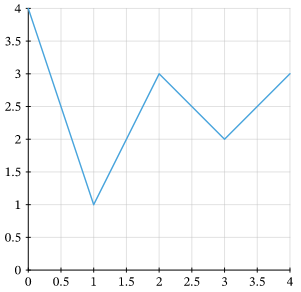
\includegraphics[scale=0.7]{Nagwa_Q2_kin2.png}
\end{figure}
%
What was the \textbf{greatest speed}, in \textbf{meters per minute} (\textbf{m/min}), at which the kite was moving? Was it descending or ascending?
%
\begin{itemize}
    \item[A. ] 3 m/min, ascending.
    \item[B. ] 4 m/min, ascending
    \item[C. ] 3 m/min, descending
    \item[D. ] 4 m/min, descending
    \item[E. ] 2 m/min, descending
\end{itemize}
%
% \begin{solution}
% We can clearly identify on the graph 4 different slopes i.e. 4 different speeds. Let us calculate the slopes.
% \begin{equation*}
%     \text{Slope}=\frac{\text{Rise $y$ axis}}{\text{Run $x$ axis}}
% \end{equation*}
% \textbf{\underline{From 0 to 3 hours the speed was:}}
% \begin{equation*}
%     \text{Speed}=\text{Slope}=\frac{\text{Rise $y$ axis}}{\text{Run $x$ axis}}=\frac{\km{18}-\km{0}}{\hours{3}-\hours{0}}=\frac{\km{18}}{\hours{3}}=\kmh{6}
% \end{equation*}
% \textbf{\underline{From 3 to 5 hours the speed was:}}
% \begin{equation*}
%     \text{Speed}=\text{Slope}=\frac{\text{Rise $y$ axis}}{\text{Run $x$ axis}}=\frac{\km{24}-\km{18}}{\hours{5}-\hours{3}}=\frac{\km{6}}{\hours{2}}=\kmh{3}
% \end{equation*}
% \textbf{\underline{From 5 to 9 hours the speed was:}}
% \begin{equation*}
%     \text{Speed}=\text{Slope}=\frac{\text{Rise $y$ axis}}{\text{Run $x$ axis}}=\frac{\km{28}-\km{24}}{\hours{9}-\hours{5}}=\frac{\km{4}}{\hours{4}}=\kmh{1}
% \end{equation*}
% \textbf{\underline{From 9 to 15 hours the speed was:}}
% \begin{equation*}
%     \text{Speed}=\text{Slope}=\frac{\text{Rise $y$ axis}}{\text{Run $x$ axis}}=\frac{\km{30}-\km{28}}{\hours{15}-\hours{9}}=\frac{\km{2}}{\hours{6}}=\kmh{1/3}
% \end{equation*}
% The \textbf{speed} is always \textbf{positive} because the \textbf{distance} is always \textbf{positive}. All negative number answers are incorrect.

% From the above calculations of the speed,

% \begin{equation*}
%     \text{Fastest speed}=\kmh{6}
% \end{equation*}

% \begin{equation*}
%     \text{Slowest speed}=\kmh{1/3}
% \end{equation*}

% \begin{equation*}
%     \boxed{\text{\bf{The answer is D}}\\
%     \textbf{fastest speed:} $6$ km/h, \textbf{slowest speed:} $1/3$ km/h.}
% \end{equation*}

% \end{solution}
%















\item The given graph shows the \textbf{distance} traveled against \textbf{time}. Which of the following statements is \textbf{not true}? \cite{Nagwa} Q. 3 \href{https://www.nagwa.com/en/worksheets/932192593730/}{Lesson Worksheet: Distance-Time Graphs}
%
\begin{figure}[H]
    \centering
    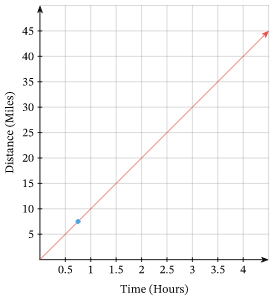
\includegraphics[scale=0.7]{Nagwa_Q3_kin2.png}
\end{figure}
%
\begin{itemize}
    \item[A. ] Any point of $\bm{(x,y)}$ coordinates on this graph means that the \textbf{distance} traveled in $\bm x$ \textbf{hours} is $\bm y$ \textbf{miles}.
    \item[B. ] It takes \textbf{10 hours} to bike \textbf{1 mile}.
    \item[C. ] The \textbf{distance} traveled in \textbf{7 hours} is \textbf{70 miles}.
    \item[D. ] The \textbf{speed} is \textbf{10 miles per hour}.
    \item[E. ] In \textbf{45 minutes}, the distance traveled is \textbf{7.5 miles}.
\end{itemize}
%
% \begin{solution}
% The speed showed in the graph is homogeneous because it is a straight line. The speed is:
% \begin{equation*}
%     \text{Speed}=\text{Slope}=\frac{\text{Rise}}{\text{Run}}=\frac{\mile{40}}{\hours{4}}=\mih{10}
% \end{equation*}
% \begin{itemize}
%     \item[] \textbf{A.} It is true. 
%     \item[] \textbf{B.} \textbf{NOT TRUE} as the speed is $\mih{10}$.
%     \item[] \textbf{C.} It is true, as the speed is $\mih{10}$.
%     \item[] \textbf{D.} It is true, as the speed is $\mih{10}$.
%     \item[] \textbf{E.} It is true, as the speed is $\mih{10}$,
%     \begin{equation*}
%         \text{Speed}=\frac{\mile{7.5}}{\hours{0.75}}=\mih{10}
%     \end{equation*}
% \end{itemize}
% \begin{equation*}
%     \boxed{\text{The answer is \textbf{B}.}}
% \end{equation*}

% \end{solution}










\item Emily walks \textbf{300 m} from her home to a cafe in \textbf{10 min}. She spends \textbf{15 min} at the cafe and then gets back home in \textbf{7 min}. \cite{Nagwa} Q. 4 \href{https://www.nagwa.com/en/worksheets/932192593730/}{Lesson Worksheet: Distance-Time Graphs}

After drawing the \textbf{distance-time} graph, \textbf{calculate} the \textbf{speed}, in \textbf{metres per hour}, with which Emily walks during each part of her journey. Round your answers to the nearest hundredth, if necessary.
%
\begin{itemize}
    \item[A. ] First 10 min: \textbf{300 m/h}, next 15 min: \textbf{0 m/h}, last 7 min: \textbf{42.86 m/h}.
    \item[B. ] First 10 min: \textbf{50 m/h}, next 15 min: \textbf{0 m/h}, last 7 min: \textbf{71.43 m/h}.
    \item[C. ] First 10 min: \textbf{0.5 m/h}, next 15 min: \textbf{0 m/h}, last 7 min: \textbf{0.71 m/h}
    \item[D. ] First 10 min: \textbf{1800 m/h}, next 15 min: \textbf{0 m/h}, last 7 min: \textbf{1800 m/h}.
    \item[E. ] First 10 min: \textbf{1800 m/h}, next 15 min: \textbf{0 m/h}, last 7 min: \textbf{2571.43 m/h}
\end{itemize}
%
% \begin{solution}
% \begin{figure}[H]
%     \centering
%     \begin{tikzpicture}
% \begin{axis}[
%     title={Distance-time graph},
%     xlabel={Time [min]},
%     ylabel={Distance [m]},
%     xmin=0, xmax=35,
%     ymin=0, ymax=650,
%     xtick={0,10,25,32},
%     ytick={0,300,300,600},
%     ymajorgrids=true,
%     xmajorgrids=true,
%     grid style=dashed,
%     width=0.7\textwidth
% ]

% \addplot[
%     color=blue,
%     mark=square,
%     ]
%     coordinates {
%     (0,20)(10,300)(25,300)(32,600)
%     };
% \end{axis}
% \end{tikzpicture}
% \end{figure}
% To answer the section about the speed in each interval we need to convert the time from minutes to hours as the answer is given in metres per hour.

% First 10 min to hours is:
% \begin{equation*}
%     \cgsmin{10}\cdot\frac{\hours{1}}{\cgsmin{60}}=\hours{0.167}
% \end{equation*}
% 15 min at cafe to hours is:
% \begin{equation*}
%     \cgsmin{15}\cdot\frac{\hours{1}}{\cgsmin{60}}=\hours{0.250}
% \end{equation*}
% 7 min to get back home:
% \begin{equation*}
%     \cgsmin{7}\cdot\frac{\hours{1}}{\cgsmin{60}}=\hours{0.117}
% \end{equation*}


% \textbf{\underline{Speed first 10 min:}}
% \begin{equation*}
%     \text{Speed}=\text{Slope}=\frac{\text{Rise $y$ axis}}{\text{Run $x$ axis}}=\frac{\msis{300}-\msis{0}}{\hours{0.167}-\hours{0}}=\frac{\msis{300}}{\hours{0.167}}= 1800 \msis{}/\hours{}
% \end{equation*}
% \textbf{\underline{Speed next 15 min:}}
% \begin{equation*}
%     \text{Speed}=\text{Slope}=\frac{\text{Rise $y$ axis}}{\text{Run $x$ axis}}=\frac{\msis{300}-\msis{300}}{\hours{0.417}-\hours{0.167}}=\frac{\msis{0}}{\hours{0.25}}= 0 \msis{}/\hours{}
% \end{equation*}
% \textbf{\underline{Speed last 7 min:}}
% \begin{equation*}
%     \text{Speed}=\text{Slope}=\frac{\text{Rise $y$ axis}}{\text{Run $x$ axis}}=\frac{\msis{600}-\msis{300}}{\hours{0.534}-\hours{0.417}}=\frac{\msis{300}}{\hours{0.117}}\sim  2571.42 \msis{}/\hours{}
% \end{equation*}
% \begin{equation*}
%     \boxed{\text{The answer is \textbf{E}}}
% \end{equation*}
% \end{solution}












% Easy move to begining of this section time-distance
\item The following graph shows the distance Mohammed traveled in metres. \cite{Nagwa} Q. 6 \href{https://www.nagwa.com/en/worksheets/932192593730/}{Lesson Worksheet: Distance-Time Graphs}
%
\begin{figure}[H]
    \centering
    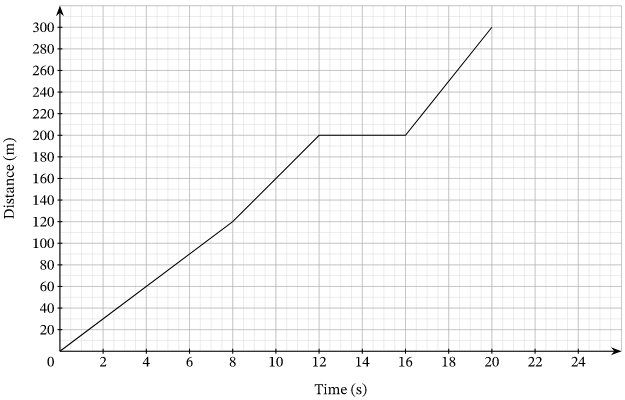
\includegraphics[scale=0.7]{Nagwa_Q6_kin2.png}
\end{figure}
%
\begin{itemize}
    \item[\bf (a)] \textbf{How far} has Mohammed traveled after \textbf{8 seconds}?
    %
    % \begin{solution}
    % Looking at the graph one can infer that the distance was,
    % \begin{equation*}
    %     \boxed{\text{Distance}=\msis{120}}
    % \end{equation*}
    % \end{solution}
    %
    \item[\bf (b)] \textbf{How far} has Mohammed traveled after \textbf{14 seconds}?
    %
    % \begin{solution}
    % Looking at the graph one can infer that the distance was,
    % \begin{equation*}
    %     \boxed{\text{Distance}=\msis{200}}
    % \end{equation*}
    % \end{solution}
    %
\end{itemize}














\item A driver keeps records of \textbf{distances} he covers with his truck (the truck stays at rest between shifts). \cite{Nagwa} Q. 7 \href{https://www.nagwa.com/en/worksheets/932192593730/}{Lesson Worksheet: Distance-Time Graphs}
%
\begin{figure}[H]
    \centering
    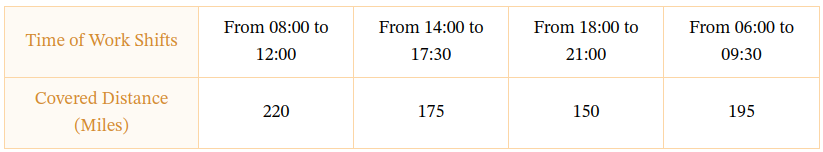
\includegraphics[width=0.7\textwidth]{Nagwa_Q7_kin2.png}
\end{figure}
%
\begin{itemize}
    \item[\bf (a)] \textbf{Draw} the \textbf{distance-time} graph.
    %
%     \begin{solution}
%     \begin{figure}[H]
%     \centering
%     \begin{tikzpicture}
% \begin{axis}[
%     title={Truck distance-time graph},
%     xlabel={Clock time [hours:min]},
%     ylabel={Distance [miles]},
%     xmin=0, xmax=26,
%     ymin=0, ymax=750,
%     xtick={0,4,6,9.5,10,13,22,25.5},
%     xticklabels={$8$, $12$, $14$, $17:30$, $18$, $21$, $6$, $9:30$},
%     ytick={0,220,395,545,740},
%     ymajorgrids=true,
%     xmajorgrids=true,
%     grid style=dashed,
%     width=0.7\textwidth
% ]

%     \addplot[
%     color=blue,
%     mark=square,
%     ]
%     coordinates {
%     (0,0)(4,220)(6,220)(9.5,395)(10,395)(13,545)(22,545)(25.5,740)
%     };
%     \addplot[
%     color=red, dashed,
%     ]
%     coordinates {
%     (0,0)(25.5,740)
%     };
% \end{axis}
% \end{tikzpicture}
% \end{figure}
%     \end{solution}
    %
    \item[\bf (b)] \textbf{Calculate} the \textbf{average speed} of the truck from \textbf{8:00} to \textbf{9:30} the \textbf{next day}. Give your answer in \textbf{miles per hour}, to one decimal place.
    %
    % \begin{solution}
    % The average speed is the total distance divided by the total time. The average speed corresponds to the slope of the red dashed line plotted in the previous graph.
    % \begin{equation*}
    %     \boxed{\text{Average Speed}=\text{Slope}=\frac{\text{Total distance}}{\text{Total time}}=\frac{\mile{740}}{\hours{25.5}}=\mih{29}}
    % \end{equation*}
    % \end{solution}
    %
\end{itemize}

















\item The given graph shows the \textbf{distance} traveled by a \textbf{sound wave}. Find the \textbf{speed of the sound}.  \cite{Nagwa} Q. 7 \href{https://www.nagwa.com/en/worksheets/932192593730/}{Lesson Worksheet: Distance-Time Graphs}
%
\begin{figure}[H]
    \centering
    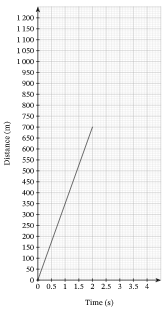
\includegraphics[scale=1]{Nagwa_Q8_kin2.png}
\end{figure}
%
% \begin{solution}
% The wave speed is the slope of the graph,
% \begin{equation*}
%         \boxed{\text{Sound  Speed}=\text{Slope}=\frac{\text{Total distance}}{\text{Total time}}=\frac{\msis{700}}{\tsis{2}}=\vsis{350}}
% \end{equation*}
% Which is compatible with the actual speed of sound in air.
% \end{solution}











\section*{\textcolor{red}{Displacement-time graphs. Velocity vs Speed.}}












\item \textbf{Which} of the following \textbf{quantities} is equal to the \textbf{slope} or \textbf{gradient} of the type of graph shown? \cite{Nagwa} Q. 1 Lesson Worksheet: Kinematic Graphs

\begin{figure}[H]
    \centering
    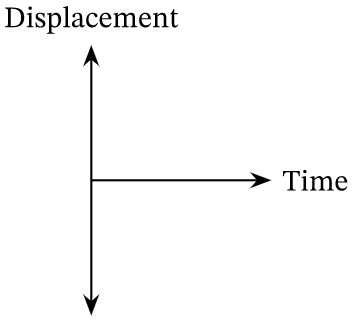
\includegraphics{Nagwa_q1_kingraph.png}
    \caption{}
    \label{fig:my_label}
\end{figure}

\begin{itemize}
    \item[A.] Velocity
    %Solution Down
    %\item[\textcolor{blue}{\bf A.}] \textcolor{blue}{\bf Velocity}
    \item[B.] Distance
    \item[C.] Acceleration
    \item[D.] Change in velocity
    \item[E.] Speed
\end{itemize}










\item The change in \textbf{displacement} of two objects with time is shown in the graph. The lines plotted on the graph are parallel. \cite{Nagwa} Q. 1 \href{https://www.nagwa.com/en/worksheets/715142164735/}{Lesson Worksheet: Graphing Velocity}
%
\begin{figure}[H]
    \centering
    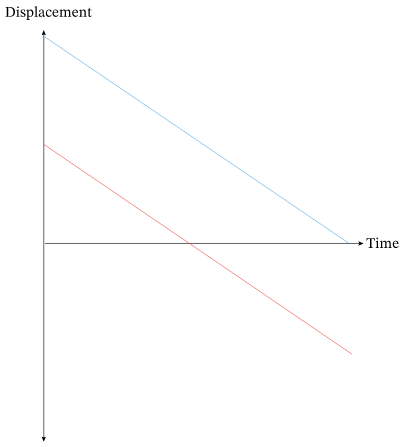
\includegraphics[scale=0.7]{Nagwa_Q1_disp.png}
\end{figure}
%
\begin{itemize}
    \item[\bf (a)] Do the two objects have the \textbf{same} \textbf{velocity}?
    %
    % \begin{solution}
    % The graphs start at $t=0$ at different displacements. The two objects start at \textbf{DIFFERENT} initial positions but the gradient or slope of the graph is the \textbf{SAME} for both graphs as the graphs are parallel.
    
    % The \textbf{gradient} or \textbf{slope} of the \textbf{displacement-time} graph is the \textbf{VELOCITY}, therefore both objects have the \textbf{SAME VELOCITY}.
    % \begin{equation*}
    %     \boxed{\text{Both objects have the same velocity (because of the same slope)}}
    % \end{equation*}
    % \end{solution}
    %
    \item[\bf (b)] Do the two objects have the \textbf{same} \textbf{speed}?
        %
    % \begin{solution}
    % The graphs show the \textbf{displacement-time} graph. The speed is normally calculated form the \textbf{distance-time} graph. However, the speed can be also calculated from the \textbf{displacement-time} graph taking the positive value or absolute value of the velocity.
    
    % Hence, the absolute value \textbf{gradient} or \textbf{slope} of the \textbf{displacement-time} graph is the \textbf{SPEED}, as the graphs are parallel have the same gradient or slope and therefore the same \textbf{SPEED}.
    % \begin{equation*}
    %     \boxed{\text{Both objects have the same speed (because of the same slope)}}
    % \end{equation*}
    % \end{solution}
    %
\end{itemize}











% Move in front of the previous one
\item The changes of \textbf{displacement} of two objects with time is shown in the graph. The lines plotted on the graph are \textbf{parallel}. \cite{Nagwa} Q. 2 \href{https://www.nagwa.com/en/worksheets/715142164735/}{Lesson Worksheet: Graphing Velocity}
%
\begin{figure}[H]
    \centering
    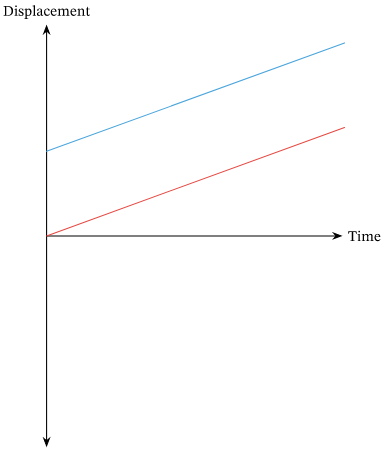
\includegraphics[scale=0.7]{Nagwa_Q2_disp.png}
\end{figure}
%
\begin{itemize}
    \item[\bf (a)] Do the two objects have the \textbf{same} \textbf{velocity}?
    %
    % \begin{solution}
    % The graphs start at $t=0$ at different displacements. The two objects start at \textbf{DIFFERENT} initial positions but the gradient or slope of the graph is the \textbf{SAME} for both graphs as the graphs are parallel.
    
    % The \textbf{gradient} or \textbf{slope} of the \textbf{displacement-time} graph is the \textbf{VELOCITY}, therefore both objects have the \textbf{SAME VELOCITY}.
    % \begin{equation*}
    %     \boxed{\text{Both objects have the same velocity (because of the same slope)}}
    % \end{equation*}
    % \end{solution}
    %
    \item[\bf (b)] Do the two objects have the \textbf{same} \textbf{speed}?
        %
    % \begin{solution}
    % The graphs show the \textbf{displacement-time} graph. The speed is normally calculated form the \textbf{distance-time} graph. However, in this case the \textbf{displacement-time} graph and \textbf{distance-time} graph are identical because the \textbf{VELOCITY} is \textbf{POSITIVE}.
    
    % Hence, the \textbf{gradient} or \textbf{slope} of the \textbf{displacement-time} graph is \textbf{ALSO} the \textbf{SPEED}. As the graphs are parallel have the same gradient or slope and therefore the same \textbf{SPEED}.
    % \begin{equation*}
    %     \boxed{\text{Both objects have the same speed (because of the same slope)}}
    % \end{equation*}
    % \end{solution}
    %
\end{itemize}













\item The \textbf{change} in \textbf{displacement} of two objects with time is shown in the graph. The gray arrows in the diagram are the \textbf{same length}. \cite{Nagwa} Q. 4 \href{https://www.nagwa.com/en/worksheets/715142164735/}{Lesson Worksheet: Graphing Velocity}
%
\begin{figure}[H]
    \centering
    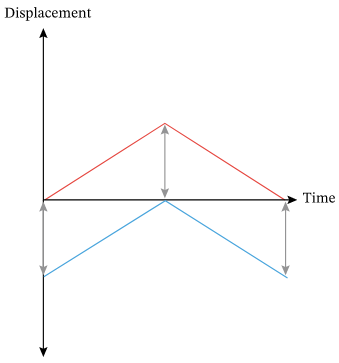
\includegraphics[scale=0.7]{Nagwa_Q4_disp.png}
\end{figure}
%
\begin{itemize}
    \item[\bf (a)] Do the two objects have the \textbf{same} \textbf{velocity}?
    %
    % \begin{solution}
    % Two regimes (trends) are shown in both graphs. A part with positive slope at the beginning (left), and a part with negative slope at the end (right).
    
    % Both graphs have the same slope in the same intervals first negative and then positive. As the slope or gradient is the velocity, both objects have the same velocity in the same time intervals.
    % \begin{equation*}
    %     \boxed{\text{\bf Both objects have the same velocity in each of the 2 time intervals}}
    % \end{equation*}
    % \end{solution}
    %
    \item[\bf (b)] Do the two objects have the \textbf{same} \textbf{speed}?
    %
    % \begin{solution}
    % Because of the same length of the grey arrows and the same initial and final points, we can infer that the absolute value of the slope in the first and second regime (positive and negative slope) is the same.
    
    % The absolute value of the slope or gradient of the displacement time graph is the speed. therefore the speed does not change in the whole time interval and is the same for both objects.
    % \begin{equation*}
    %     \boxed{\text{\bf Both objects have the same speed, and does not change in the whole time interval}}
    % \end{equation*}
    % \end{solution}
    %
\end{itemize}













\item The change in \textbf{displacement} of two objects with time is shown in the graph. The grey arrows in the diagram are the \textbf{same length}. \cite{Nagwa} Q. 5 \href{https://www.nagwa.com/en/worksheets/715142164735/}{Lesson Worksheet: Graphing Velocity}
%
\begin{figure}[H]
    \centering
    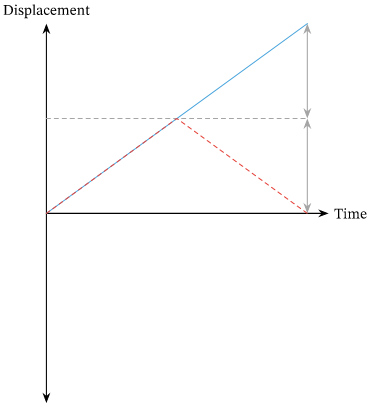
\includegraphics[scale=0.7]{Nagwa_Q5_disp.png}
\end{figure}
%
\begin{itemize}
    \item[\bf (a)] Do the two objects have the \textbf{same} \textbf{velocity}?
    %
    % \begin{solution}
    % The blue graph has the same trend over the time interval.
    
    % The red graph shows two trends. A part with positive slope at the beginning (left), and a part with negative slope at the end (right).
    
    % Both graphs have the same positive slope in the first interval. 
    
    % The graphs have different slope in the second interval, as the slope becomes negative for the red graph.
    
    % The velocity is the slope of the graph. Therefore we can assure that the velocity is ONLY the same in the first time interval. The velocity is different for both graphs in the second time interval. In general the velocity is different.
    % \begin{equation*}
    %     \boxed{\text{\bf Both objects have different velocity (same velocity only in first time interval)}}
    % \end{equation*}
    % \end{solution}
    %
    \item[\bf (b)] Do the two objects have the \textbf{same} \textbf{speed}?
    %
    % \begin{solution}
    % The absolute value of the velocity is the speed.
    
    % Grey arrows have the same length so the absolute value of the slope is the same in the whole interval.
    % \begin{equation*}
    %     \boxed{\text{\bf Both objects the same speed, and does not change in the whole time interval}}
    % \end{equation*}
    % \end{solution}
    %
\end{itemize}










% Move this one before the previous one.
\item The change in the \textbf{displacement} of two objects with time is shown in the graph. The grey arrows in the diagram are the \textbf{same length}. \cite{Nagwa} Q. 6 \href{https://www.nagwa.com/en/worksheets/715142164735/}{Lesson Worksheet: Graphing Velocity}
%
\begin{figure}[H]
    \centering
    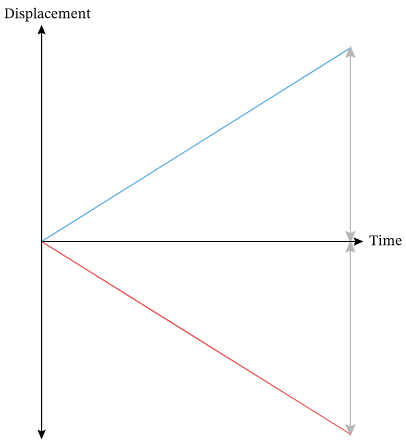
\includegraphics[scale=0.7]{Nagwa_Q6_disp.png}
\end{figure}
%
\begin{itemize}
    \item[\bf (a)] Do the two objects have the \textbf{same} \textbf{velocity}?
    %
    % \begin{solution}
    % The slope of the displacement-time graph is the velocity.
    
    % The blue graph has \textbf{positive} slope.
    
    % The red graph has \textbf{negative} slope.
    
    % The graphs have \textbf{different slope}, and therefore \textbf{different velocity}.
    % \begin{equation*}
    %     \boxed{\text{\bf Both objects have different velocity}}
    % \end{equation*}
    % \end{solution}
    %
    \item[\bf (b)] Do the two objects have the \textbf{same} \textbf{speed}?
    %
    % \begin{solution}
    % The absolute slope of the displacement-time graph is the speed.
    
    % The length of the grey arrow is the same. the time intervals for both objects are the same, therefore, the absolute value of the slope is the same.
    % \begin{equation*}
    %     \text{Speed}=\text{Absolute value of slope}=\frac{\text{Length of grey arrow}}{\text{time interval}}
    % \end{equation*}
    
    % Consequently, both objects have the same speed.
    
    % \begin{equation*}
    %     \boxed{\text{\bf Both objects have the same speed}}
    % \end{equation*}
    % \end{solution}
    %
\end{itemize} 









% move somewhere to the beginning of this section
\item The change in the \textbf{displacement} of two objects with time is shown in the graph. The grey arrows in the diagram are the \textbf{same length}. \cite{Nagwa} Q. 7 \href{https://www.nagwa.com/en/worksheets/715142164735/}{Lesson Worksheet: Graphing Velocity}
%
\begin{figure}[H]
    \centering
    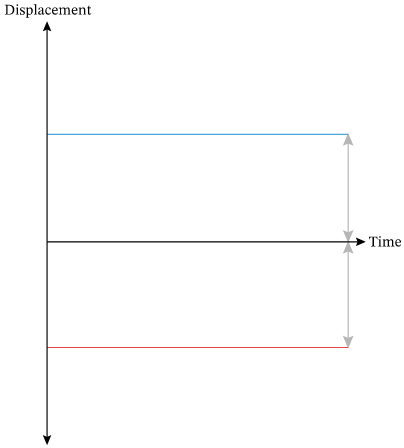
\includegraphics[scale=0.7]{Nagwa_Q7_disp.png}
\end{figure}
%
\begin{itemize}
    \item[\bf (a)] Do the two objects have the \textbf{same} \textbf{velocity}?
    %
    % \begin{solution}
    % The slope of the displacement-time graph is the velocity.
    
    % Both graphs have zero slope. Therefore, the same velocity.
    
    % \begin{equation*}
    %     \boxed{\text{\bf Both objects have same velocity}}
    % \end{equation*}
    % \end{solution}
    %
    \item[\bf (b)] Do the two objects have the \textbf{same} \textbf{speed}?
    %
    % \begin{solution}
    % If the velocity is the same the speed is always also the same.
    
    % The absolute value of the slope of the displacement-time graph is the speed.
    
    % Both graphs have zero slope. Therefore, the same speed.
    
    % \begin{equation*}
    %     \boxed{\text{\bf Both objects have same speed}}
    % \end{equation*}
    % \end{solution}
    %
\end{itemize} 












% move after 37 is very similar... same answer
\item The change of \textbf{displacement} of two objects with time is shown in the graph. The lines plotted on the graph are \textbf{parallel}. \cite{Nagwa} Q. 9 \href{https://www.nagwa.com/en/worksheets/715142164735/}{Lesson Worksheet: Graphing Velocity}
%
\begin{figure}[H]
    \centering
    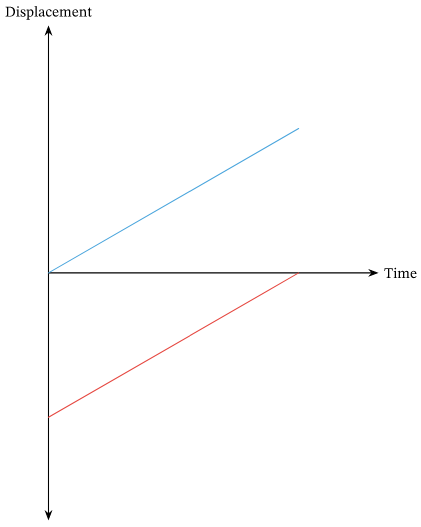
\includegraphics[scale=0.7]{Nagwa_Q9_disp.png}
\end{figure}
%
\begin{itemize}
    \item[\bf (a)] Do the two objects have the \textbf{same} \textbf{velocity}?
    %
    % \begin{solution}
    % The graphs start at $t=0$ at different displacements. The two objects start at \textbf{DIFFERENT} initial positions but the gradient or slope of the graph is the \textbf{SAME} for both graphs as the graphs are parallel.
    
    % The \textbf{gradient} or \textbf{slope} of the \textbf{displacement-time} graph is the \textbf{VELOCITY}, therefore both objects have the \textbf{SAME VELOCITY}.
    % \begin{equation*}
    %     \boxed{\text{\bf Both objects have the same velocity (because of the same slope)}}
    % \end{equation*}
    % \end{solution}
    %
    \item[\bf (b)] Do the two objects have the \textbf{same} \textbf{speed}?
        %
    % \begin{solution}
    % The graphs show the \textbf{displacement-time} graph. The speed is normally calculated form the \textbf{distance-time} graph. However, in this case the \textbf{displacement-time} graph and \textbf{distance-time} graph are identical because the \textbf{VELOCITY} is \textbf{POSITIVE}.
    
    % Hence, the \textbf{gradient} or \textbf{slope} of the \textbf{displacement-time} graph is \textbf{ALSO} the \textbf{SPEED}. As the graphs are parallel have the same gradient or slope and therefore the same \textbf{SPEED}.
    % \begin{equation*}
    %     \boxed{\text{\bf Both objects have the same speed (because of the same slope)}}
    % \end{equation*}
    % \end{solution}
    %
\end{itemize}

















\item The graph shows the \textbf{displacement} covered in kilometres by a vehicle that set off and returned \textbf{back} to its \textbf{initial position} (vertical axis). The horizontal axis represents the time in minutes. \cite{Nagwa} Q. 5 \href{https://www.nagwa.com/en/worksheets/932192593730/}{Lesson Worksheet: Distance-Time Graphs}
%
\begin{figure}[H]
    \centering
    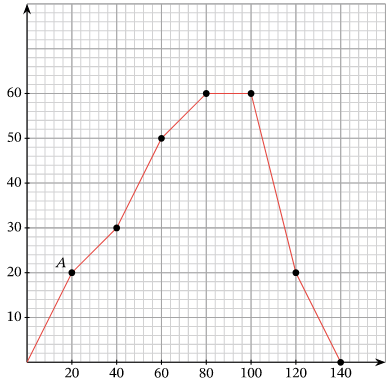
\includegraphics[scale=1]{Nagwa_Q5_kin2.png}
\end{figure}
%
\begin{itemize}
    \item[\bf (a)] What happened at point \textbf{A}?
    %
    \begin{example}
    At point \textbf{A}, the slope (or gradient) of the displacement-time graph changes. This is indicating a change in the speed. As the slope does not change the sign is just a change in the magnitude of the velocity (also a change of the speed).
    \end{example}
    %
    \item[\bf (b)] \textbf{How long} after setting off did the vehicle \textbf{first stop}?
    %
    \begin{example}
    A displacement-time graph shows that the movement has stopped if the slope of the graph is zero (a region where the graph is horizontal i.e. flat). If you observe the graph this clearly happens between times:\\
    \begin{equation*}
        \text{The vehicle is stopped from minute 80 until minute 100.}
    \end{equation*}
    therefore,
    \begin{equation*}
        \boxed{\text{The vehicle stops after \textbf{80 minutes} of the departure.}}
    \end{equation*}
    \end{example}
    %
     \item[\bf (c)] \textbf{Calculate} the \textbf{average speed} for the whole journey. Give your answer in kilometres per hour and round to one decimal place.
     %
     \begin{example}
     The average speed is the total distance gone by the vehicle. The vehicle does a round trip, the \textbf{total distance} gone by the vehicle:
     \begin{equation*}
         \text{Total distance}=\km{60}+\km{60}=\km{120}
     \end{equation*}
     The total time taken to cover the round trip is:
     \begin{equation*}
         \text{Total time}=\mincgs{140}=\hours{2.33}
     \end{equation*}
     therefore the \textbf{average speed} is:
     \begin{equation*}
         \boxed{\text{Speed}=\frac{\text{Total distance}}{\text{Total time}}=\frac{\km{120}}{\hours{2.33}}=\kmh{51.5}}
     \end{equation*}
     \end{example}
     %
    \item[\bf (d)] \textbf{Calculate} the \textbf{average velocity} for the whole journey. Give your answer in kilometres per hour and round to one decimal place. \cite{Triguero}
    %
    \begin{example}
    The average displacement is the total displacement divided by the total time.
    
    \textbf{Total displacement} is the distance and direction from initial position to final position. As initial and final positions are the same (round trip) the total displacement is \textbf{zero} and no direction as the vehicle hasn't move between initial and final position:
     \begin{equation*}
         \text{Total displacement}=\km{0}
     \end{equation*}
     The total time taken to cover the round trip is:
     \begin{equation*}
         \text{Total time}=\mincgs{140}=\hours{2.33}
     \end{equation*}
     therefore the \textbf{average velocity} is:
     \begin{equation*}
    \boxed{\text{Velocity}=\frac{\text{Total displacement}}{\text{Total time}}=\frac{\km{0}}{\hours{2.33}}=\kmh{0}}
     \end{equation*}
    \end{example}
    %
    
\end{itemize}


















\item The following \textbf{displacement-time} graph is a plot of the \textbf{height} in \textbf{meters} of a kite over a \textbf{4-minute period} (height is vertical axis and time in horizontal axis).  \cite{Nagwa} Q. 2 \href{https://www.nagwa.com/en/worksheets/932192593730/}{Lesson Worksheet: Distance-Time Graphs}
%
\begin{figure}[H]
    \centering
    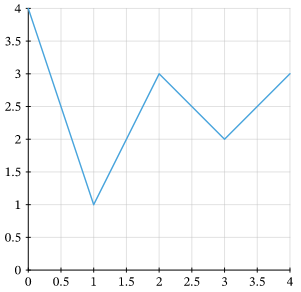
\includegraphics[scale=0.7]{Nagwa_Q2_kin2.png}
\end{figure}
%
What was the \textbf{greatest velocity}, in \textbf{meters per minute} (\textbf{m/min}), at which the kite was moving? Was it descending or ascending?
%
\begin{itemize}
    \item[A. ] 3 m/min, ascending.
    \item[B. ] 4 m/min, ascending.
    \item[C. ] 3 m/min, descending.
    \item[D. ] 4 m/min, descending.
    \item[E. ] 2 m/min, descending.
\end{itemize}
%
\begin{example}
We can clearly identify on the graph 4 different slopes i.e. 4 different velocities. Let us calculate the slopes.
\begin{equation*}
    \text{Slope}=\frac{\text{Rise $y$ axis}}{\text{Run $x$ axis}}
\end{equation*}
\textbf{\underline{From 0 to 1 minute the vertical velocity of the kite was:}}
\begin{equation*}
    \text{Speed}=\text{Slope}=\frac{\text{Rise $y$ axis}}{\text{Run $x$ axis}}=\frac{\msis{1}-\msis{4}}{\mincgs{1}-\mincgs{0}}=\frac{\msis{-3}}{\mincgs{1}}=-3 \msis{}/\mincgs{}
\end{equation*}
\textbf{The negative sign indicates the direction of the velocity. In this case means descending.}

\textbf{\underline{From 1 minute to 2 minutes the vertical velocity of the kite was:}}
\begin{equation*}
    \text{Speed}=\text{Slope}=\frac{\text{Rise $y$ axis}}{\text{Run $x$ axis}}=\frac{\msis{3}-\msis{1}}{\mincgs{2}-\mincgs{1}}=\frac{\msis{2}}{\mincgs{1}}=2 \msis{}/\mincgs{}
\end{equation*}
\textbf{The positive sign indicates the direction of the velocity. In this case means ascending.}

\textbf{\underline{From 2 minute to 3 minutes the vertical velocity of the kite was:}}
\begin{equation*}
    \text{Speed}=\text{Slope}=\frac{\text{Rise $y$ axis}}{\text{Run $x$ axis}}=\frac{\msis{2}-\msis{3}}{\mincgs{3}-\mincgs{2}}=\frac{\msis{-1}}{\mincgs{1}}=-1 \msis{}/\mincgs{}
\end{equation*}
\textbf{Again, the negative sign indicates the direction of the velocity. In this case means descending.}


\textbf{\underline{From 3 minute to 4 minutes the vertical velocity of the kite was:}}
\begin{equation*}
    \text{Speed}=\text{Slope}=\frac{\text{Rise $y$ axis}}{\text{Run $x$ axis}}=\frac{\msis{3}-\msis{2}}{\mincgs{4}-\mincgs{3}}=\frac{\msis{1}}{\mincgs{1}}=1 \msis{}/\mincgs{}
\end{equation*}
\textbf{The positive sign indicates that the kite is ascending.}

From the above calculations of the velocity,

\begin{equation*}
    \boxed{\text{\bf{The answer is C. }}
    \textbf{ Greatest velocity was: } \bm{3} \text{\textbf{ m/min, and the direction was descending.}}}
\end{equation*}
\end{example}
%


































\item {\it Key problem:} John makes a \textbf{return journey} to his local shop to buy a newspaper. In Figure~\ref{jocox}, \textbf{Graph A} is the \textbf{distance-time} graph and \textbf{Graph B} is the \textbf{displacement-time} graph for the journey. \cite{CCEADA,Triguero} p. 356 pb. 12
%
\begin{itemize}
    \item[\bf (a)] Copy and complete \textbf{Graph B}.
    %
    \begin{figure}[H]
    \centering
    \begin{tikzpicture}
    \begin{axis}[title={\bf Graph A},height=7cm,width=8cm,grid=major,xlabel={time, $t$[s]},ylabel={\textcolor{red}{Distance, $d$[cm]}}]
	\addplot[black,line width=1.0mm] coordinates {
		(0,0)
		(100,100)
		(200,200)
		(300,200)
		(600,400)
	};
	\end{axis}
    \end{tikzpicture}
    %
    \begin{tikzpicture}
    \begin{axis}[title={\bf Graph B},height=7cm,width=8cm,grid=major,xlabel={time, $t$[s]},ylabel={\textcolor{blue}{Displacement, $\vec{d}$[cm]}}]
	\addplot[black,line width=1.0mm] coordinates {
		(0,0)
		(100,100)
		(200,200)
		(300,200)
	};
	\addplot[white,dashed,line width=0.0mm] coordinates {
		(0,0)
		(600,400)
	};
	%
	% BEGIN SOLUTION
	%
% 	\addplot[blue,line width=1.0mm] coordinates {
% 		(300,200)
% 		(600,0)
% 	};
	%
	% END SOLUTION
	%
	\end{axis}
    \end{tikzpicture}
    \caption{{\bf Graph A:} Distance-time graph. {\bf Graph B:} Displacement-time graph.}
    \label{jocox}
    \end{figure}
    %
    \item[\bf (b)] What is the \textbf{average velocity} for John's journey?
    %
    % \begin{solution}
    % The \textbf{average velocity} is the \textbf{slope} of the \textbf{displacement-time} graph (GRAPH B) \textbf{between} the \textbf{initial} and \textbf{final} \textbf{displacements}:
    % \begin{equation*}
    %     \text{velocity John}=\frac{\text{total displacement}}{\text{time}}=\frac{\vec{d}}{t}=\frac{\cmcgs{0}}{\tsis{600}}=0 \cmcgs{}/\tsis{}
    %     \end{equation*}
    %     \begin{equation*}
    %     \boxed{
    %         \text{\bf John average velocity is 0} \cmcgs{}/\tsis{}}
    % \end{equation*}
    % Note: Check the graph to show displacement 0.
    % \end{solution}
    %
    \item[\bf (c)] What is the \textbf{average speed} for John's journey?
    %
%   \begin{solution}
%     The \textbf{average speed} is the \textbf{slope} of the \textbf{distance-time} graph (GRAPH A) \textbf{between} the \textbf{initial} and \textbf{final} \textbf{distance}:
%     \begin{equation*}
%         \text{speed John}=\frac{\text{total distance}}{\text{time}}=\frac{d}{t}=\frac{\cmcgs{400}}{\tsis{600}}=0.67 \cmcgs{}/\tsis{}
%         \end{equation*}
%         \begin{equation*}
%         \boxed{
%             \text{\bf John average speed is 0.67} \cmcgs{}/\tsis{}}
%     \end{equation*}
%     Note: Check the graph to show displacement 0.
%     \end{solution}
    %
\end{itemize}
























\item The diagram on Figure~\ref{pag31prob2} shows a {\bf displacement-time} graph for a moving object. \cite{ASCCEA} pag. 31 prob. 2
%
\begin{figure}[H]
    \centering
    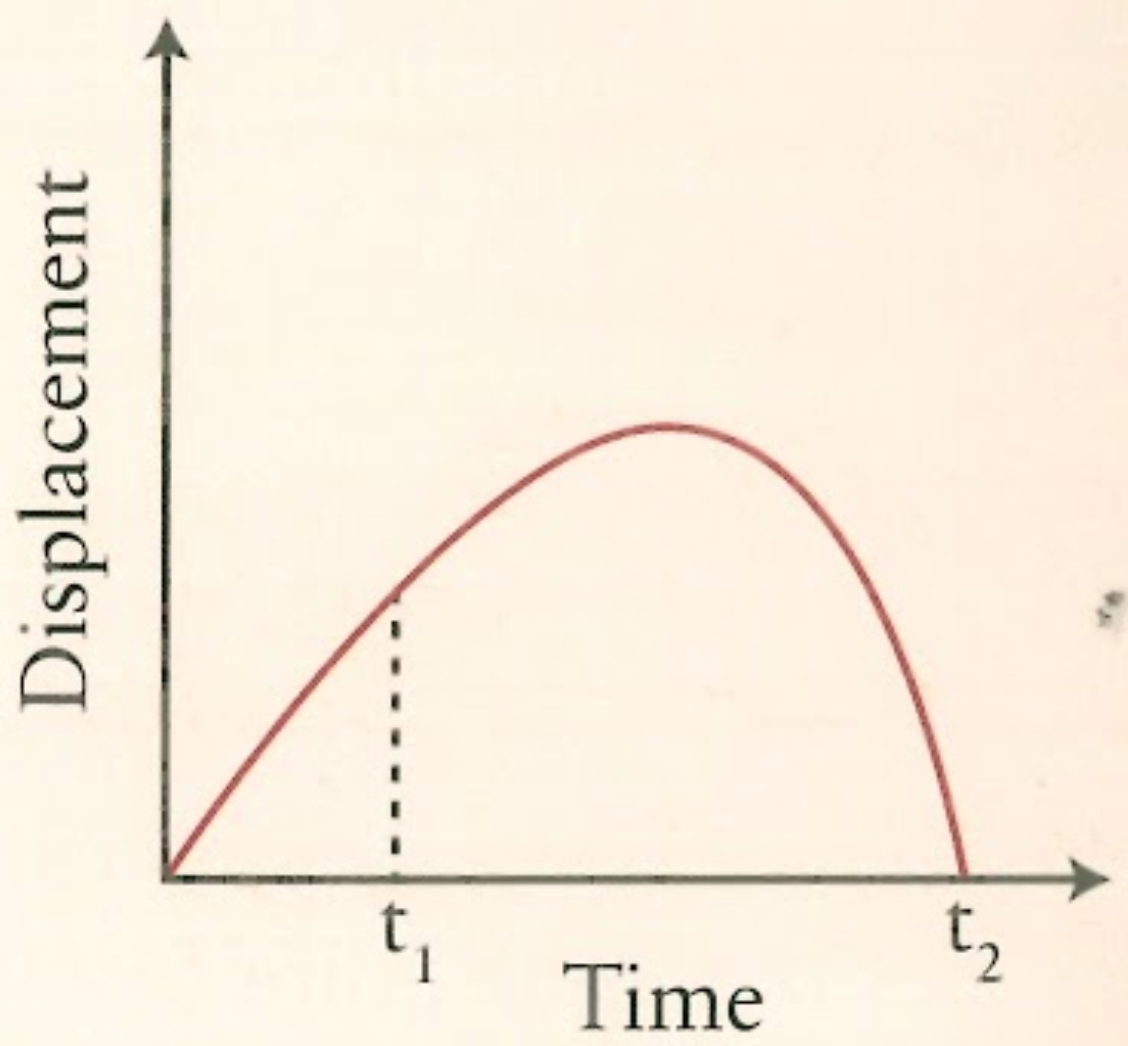
\includegraphics[scale=0.3]{pag31prob2.png}
    \caption{}
    \label{pag31prob2}
\end{figure}
%
\begin{itemize}
\item[\bf (a)] \textbf{Explain} how the velocity of the object at time $\bm{t_1}$, could be obtained from the graph.
    %
%   \begin{solution}
%     Calculating the \textbf{slope} of the displacement-time graph at that point $t_1$. This is the slope of the tangent to that point.
%     \end{solution}
    %
\item[\bf (b)] What is the \textbf{average velocity} for the journey from the \textbf{beginning} to time $\bm{t_2}$?
    %
    % \begin{solution}
    % Given that the \textbf{total displacement} is \textbf{zero}. The \textbf{rate of change} of the \textbf{displacement} with respect to the \textbf{time} is then \textbf{zero}.
    % \begin{equation*}
    %     \boxed{\text{The \textbf{average velocity} between the \textbf{beginning} and $\bm{t_2}$ is \textbf{ZERO}.}}
    % \end{equation*}
    % \end{solution}
    %
\end{itemize}

















% \item \href{https://isaacphysics.org/questions/hare_tortoise_race?board=72ae6868-9544-47c3-a068-786d3fc0ddd5}{\it The Hare and the Tortoise:} A hare and a tortoise are having a race along a {\bf 2.0 km} track. The tortoise sets off at a constant speed of {\bf 1.6 ms}$\bm{^{-1}}$. The hare is confident that he can win and so naps for {\bf 15 minutes} before setting off at {\bf 5.0 ms}$\bm{^{-1}}$. \cite{Jardine-Wright}
% %
% \begin{itemize}
% \item[\bf (a)] {\it Distance-time graph:} Draw a {\bf distance-time graph}, to scale, showing both the hare and the tortoise to \textbf{find out who will win the race}.
% %
% %
% \begin{figure}[H]
%     \centering
%     \scalebox{1.7}{
%     \begin{tikzpicture}
% \begin{axis}[ticklabel style={/pgf/number format/1000 sep=},line width=1.2,
% 	axis x line=bottom,
% 	axis y line=left,
% 	xlabel=$\text{Time, }t\,\text{[s]}$,ylabel=$\text{Distance, }x\,\text{[m]}$,grid=both]
% % %
% % %
% % % The HARE
% % %
% %        blue/white
% \addplot[blue,mark=none,
% 	 domain=0:900,y domain=0:2000,line width=1,samples=2,color=blue] %blue/white
% 	{0};
% 	%     red/white
% \addplot[red,mark=none,
% 	 domain=900:1300,y domain=0:38,line width=1,samples=2,color=red] %white/red
% 	{5*(x-900)};
% % % The HARE
% % %
% \addplot[blue,mark=none,
% 	 domain=0:900,y domain=0:2000,line width=1,samples=2,color=red]
% 	{0};
% \addplot[red,mark=none,
% 	 domain=850:1250,y domain=0:38,line width=1,samples=2,color=gray]
% 	{5*(x-850)};
% %
% %
% % The TORTOISE
% %
% \addplot[blue,mark=none,
% 	 domain=0:1250,y domain=0:2000,samples=2,line width=1,color=Greenss]%Greenss/white
% 	{1.6*x};
% % %
% % %
% % % REFERENCE FINISH
% % %
% \addplot[blue,mark=none,
% 	 domain=0:1400,y domain=0:2300,samples=2,dashed,color=gray]
% 	{2000};
% 	\addplot[blue,mark=none,
% 	 domain=0:90,y domain=0:40,samples=2,dashed,color=white]
% 	{40.0};
% %
% %
% %
% \addplot +[mark=none,dashed,color=gray] coordinates {(1250,0) (1250,2000)};
% %
% \addplot +[mark=none,dashed,color=gray] coordinates {(1300,0) (1300,2000)};
% %
% \addplot +[mark=none,dashed,color=white] coordinates {(0,2200) (1300,2200)};
% %
% \node[
% 	 domain=0:1300,y domain=0:40,color=gray] at (axis cs:650,2100) {$L=$ 2000 m}; %
% \node[
% 	 domain=-5:10,y domain=0:40,color=Greenss] at (axis cs:1250,2100) {$t_T$};
% \node[
% 	 domain=-5:10,y domain=0:40,color=red] at (axis cs:1300,2100) {$t_H$};
% \end{axis}
% \node[] at (0,5) {$L$};
% \end{tikzpicture}}
%     \caption{The Hare and the Tortoise.}
%     \label{fig:my_label}
% \end{figure}
% %
% %
% %
% %
% %
% %\begin{comment}
% \textcolor{blue}{
% \\
% {\bf (a) Solution:}\\
% Graph:\\
% \begin{figure}[H]
%     \centering
%     \scalebox{1.7}{
%     \begin{tikzpicture}
% \begin{axis}[line width=1,
% 	axis x line=bottom,
% 	axis y line=left,
% 	xlabel=$\text{Time, }t\,\text{[s]}$,ylabel=$\text{Displacement, }x\,\text{[cm]}$]
% %
% %
% % The HARE
% %
% \addplot[blue,mark=none,
% 	 domain=0:900,y domain=0:2000,line width=1,samples=2,color=red]
% 	{0};
% \addplot[red,mark=none,
% 	 domain=900:1300,y domain=0:38,line width=1,samples=2,color=red]
% 	{5*(x-900)};
% % The HARE
% %
% \addplot[blue,mark=none,
% 	 domain=0:900,y domain=0:2000,line width=1,samples=2,color=red]
% 	{0};
% \addplot[red,mark=none,
% 	 domain=850:1250,y domain=0:38,line width=1,samples=2,color=gray]
% 	{5*(x-850)};
% %
% %
% % The TORTOISE
% %
% \addplot[blue,mark=none,
% 	 domain=0:1250,y domain=0:2000,samples=2,line width=1,color=Greenss]
% 	{1.6*x+5.4};
% %
% %
% % REFERENCE FINISH
% %
% \addplot[blue,mark=none,
% 	 domain=0:1400,y domain=0:2300,samples=2,dashed,color=gray]
% 	{2000};
% 	\addplot[blue,mark=none,
% 	 domain=0:90,y domain=0:40,samples=2,dashed,color=white]
% 	{40.0};
% %
% %
% %
% \addplot +[mark=none,dashed,color=gray] coordinates {(1250,0) (1250,2000)};
% %
% \addplot +[mark=none,dashed,color=gray] coordinates {(1300,0) (1300,2000)};
% %
% \addplot +[mark=none,dashed,color=white] coordinates {(0,2200) (1300,2200)};
% %
% \node[
% 	 domain=0:1300,y domain=0:40,color=gray] at (axis cs:650,2100) {$L=$ 2000 m}; %
% \node[
% 	 domain=-5:10,y domain=0:40,color=Greenss] at (axis cs:1250,2100) {$t_T$};
% \node[
% 	 domain=-5:10,y domain=0:40,color=red] at (axis cs:1300,2100) {$t_H$};
% \node[
% 	 domain=-5:10,y domain=0:40,color=red] at (axis cs:80.4,38) {$t_A$};
% \node[above,red] at (0,37.5) {$\log_{10} 10=1$};
% \node at (axis cs:0,37.5) [anchor=north east] {test};
% \end{axis}
% %\node[] at (0,5) {$L$};
% \end{tikzpicture}}
%     \caption{}
%     \label{fig:my_label}
% \end{figure}
% %
% %
% %
% %
% \begin{equation*}
% x_T(t)=v_T\,t
% \end{equation*}
% \begin{equation*}
% x_T(t)=v_T\,(t-t_0)
% \end{equation*}
% \begin{equation*}
% x_T(t)=L \Longrightarrow t_T=\frac{L}{v_T}=\frac{2000\text{ m}}{1.6\text{ m/s}}=1250\text{ s}
% \end{equation*}
% \begin{equation*}
% x_H(t)=L\Longrightarrow t_H=\frac{L}{v_H}+t_0=\frac{2000\text{ m}}{5\text{ m/s}}+900\text{ s}=1300\text{ s}
% \end{equation*}
% }
% %
% %\end{comment}
% %
% %
% %
% %
% \item[\bf (b)] What {\bf length of the hare's nap}, in seconds, will end the race in a draw?
% %850 sec=14 min
% \end{itemize}













\item \label{smalgranuki} Complete the three small \textbf{displacement-time} graphs on the same axis from the information provided in each section. \cite{Elert,Triguero} Kinematics
%
\begin{itemize}
    \item[\bf (a)] A car started to move from displacement $\msis{0}$ at constant speed of $\vsis{1}$.
    \item[\bf (b)] A car started to move from displacement $\msis{20}$ at constant velocity of $\vsis{-1}$.
    \item[\bf (c)] A car started to move from displacement $\msis{5}$ at constant speed of $\vsis{2}$.
    \item[\bf (d)] A car started to move from displacement $\msis{25}$ at constant velocity of $\vsis{-4}$.
    \item[\bf (e)] A car started to move at time $t=\tsis{15}$ from displacement $\msis{20}$ at constant velocity of $\vsis{-3}$.
    \item[\bf (f)] A car started to move from displacement $\msis{27}$ at constant velocity of $\vsis{0}$.
\end{itemize}
%
\begin{figure}[H]
    \centering
    \begin{tikzpicture}
    \begin{axis}[
    %title={Temperature dependence of CuSO$_4\cdot$5H$_2$O solubility},
    width=0.7\textwidth,
    height=0.7\textwidth,
    xlabel={Time, $t$ [s]},
    ylabel={Displacement, $d$ [m]},
    xmin=0, xmax=30,
    ymin=0, ymax=30,
    xtick={0,5,10,15,20,25,30},
    ytick={0,5,10,15,20,25,30},
    legend pos=south east,
    grid=both,
    minor tick num=4,
    %grid style=dashed,
    ]
    %
    % FOR ANSWERS UN-COMMENT BELOW
    %
    % \addplot[color=blue,mark=none,domain=0:30,samples=2,line width=1mm]{x};
    % \addplot[color=red,mark=none,domain=0:30,samples=2,line width=1mm]{20-x};
    % \addplot[color=orange,mark=none,domain=0:30,samples=2,line width=1mm]{2*x+5};
    % \addplot[color=green,mark=none,domain=0:30,samples=2,line width=1mm]{-4*x+25};
    % %\addplot[color=black,mark=none,domain=17:30,samples=10,line width=1mm]{-3*x+27};
    % \addplot[color=black,mark=none,domain=17:30,samples=10,line width=1mm]
    % coordinates {
    % (15,20)(22,-1)
    % };
    % \addplot[color=yellow,mark=none,domain=0:30,samples=2,line width=1mm]{27};
    % \legend{\Large \bf (a),\Large \bf (b),\Large \bf (c),\Large \bf (d),\Large \bf (e),\Large \bf (f)}
    %
    % FOR ANSWERS UN-COMMENT ABOVE
    %
\end{axis}
\end{tikzpicture}
     \caption{\label{xmallii} Problem~\ref{smalgranuki}.}
\end{figure}









\item \href{https://physics.info/motion-graphs/problems.shtml}{\it Displacement:} The \href{https://physics.info/motion-graphs/worksheet-choose-displacement.pdf}{graphs} in Figure~\ref{fig:descript} show the {\bf displacement} of a hypothetical object moving along a {\bf straight line}. Choose the lettered \textbf{graph} or \textbf{graphs} that best represents each description. \cite{Elert,Triguero}\\
{\it A graph may be used for more than one description or it may not be used at all}. 
{\it Some descriptions may correspond to more than one graph and some may not correspond to any graph at all.}
\begin{itemize}
    \item[\bf (a)] The object is \textbf{moving away from} position 0 at a \textbf{constant velocity}.
    %
    % \begin{solution}
    % \begin{equation*}
    %     \boxed{\text{\bf A and H}}
    % \end{equation*}
    % \end{solution}
    %
    \item[\bf(b)] The object is \textbf{moving toward} position 0 at \textbf{constant velocity}.
    %
    % \begin{solution}
    % \begin{equation*}
    %     \boxed{\text{\bf B and C}}
    % \end{equation*}
    % \end{solution}
    %
    \item[\bf(c)] The object's \textbf{velocity} is \textbf{increasing}.% at a \textbf{uniform rate}.
    %
    % \begin{solution}
    % \begin{equation*}
    %     \boxed{\text{\bf No graph}}
    % \end{equation*}
    % \end{solution}
    %
    \item[\bf (d)] The object's \textbf{velocity} is \textbf{decreasing}.% at a \textbf{uniform rate}
    %
    % \begin{solution}
    % \begin{equation*}
    %     \boxed{\text{\bf No graph}}
    % \end{equation*}
    % \end{solution}
    %
    \item[\bf (e)] The object \textbf{changes direction}.
    %
    % \begin{solution}
    % \begin{equation*}
    %     \boxed{\text{\bf H and I}}
    % \end{equation*}
    % \end{solution}
    %
    \item[\bf (f)] The object is \textbf{standing still} for an \textbf{extended period of time}.
    %
    % \begin{solution}
    % \begin{equation*}
    %     \boxed{\text{\bf D, E, and F}}
    % \end{equation*}
    % \end{solution}
    %
    \item[\bf (g)] The object is \textbf{momentarily} (and only momentarily) \textbf{at rest} on \textbf{one occasion}.
    %
    % \begin{solution}
    % \begin{equation*}
    %     \boxed{\text{\bf H}}
    % \end{equation*}
    % \end{solution}
    %
    \item[\bf (h)] The object is \textbf{momentarily} (and only momentarily) at rest on \textbf{two or more separate occasions}.
    %
    % \begin{solution}
    % \begin{equation*}
    %     \boxed{\text{\bf G and I}}
    % \end{equation*}
    % \end{solution}
    %
\end{itemize}
%
%
\begin{figure}[H]
    \centering
    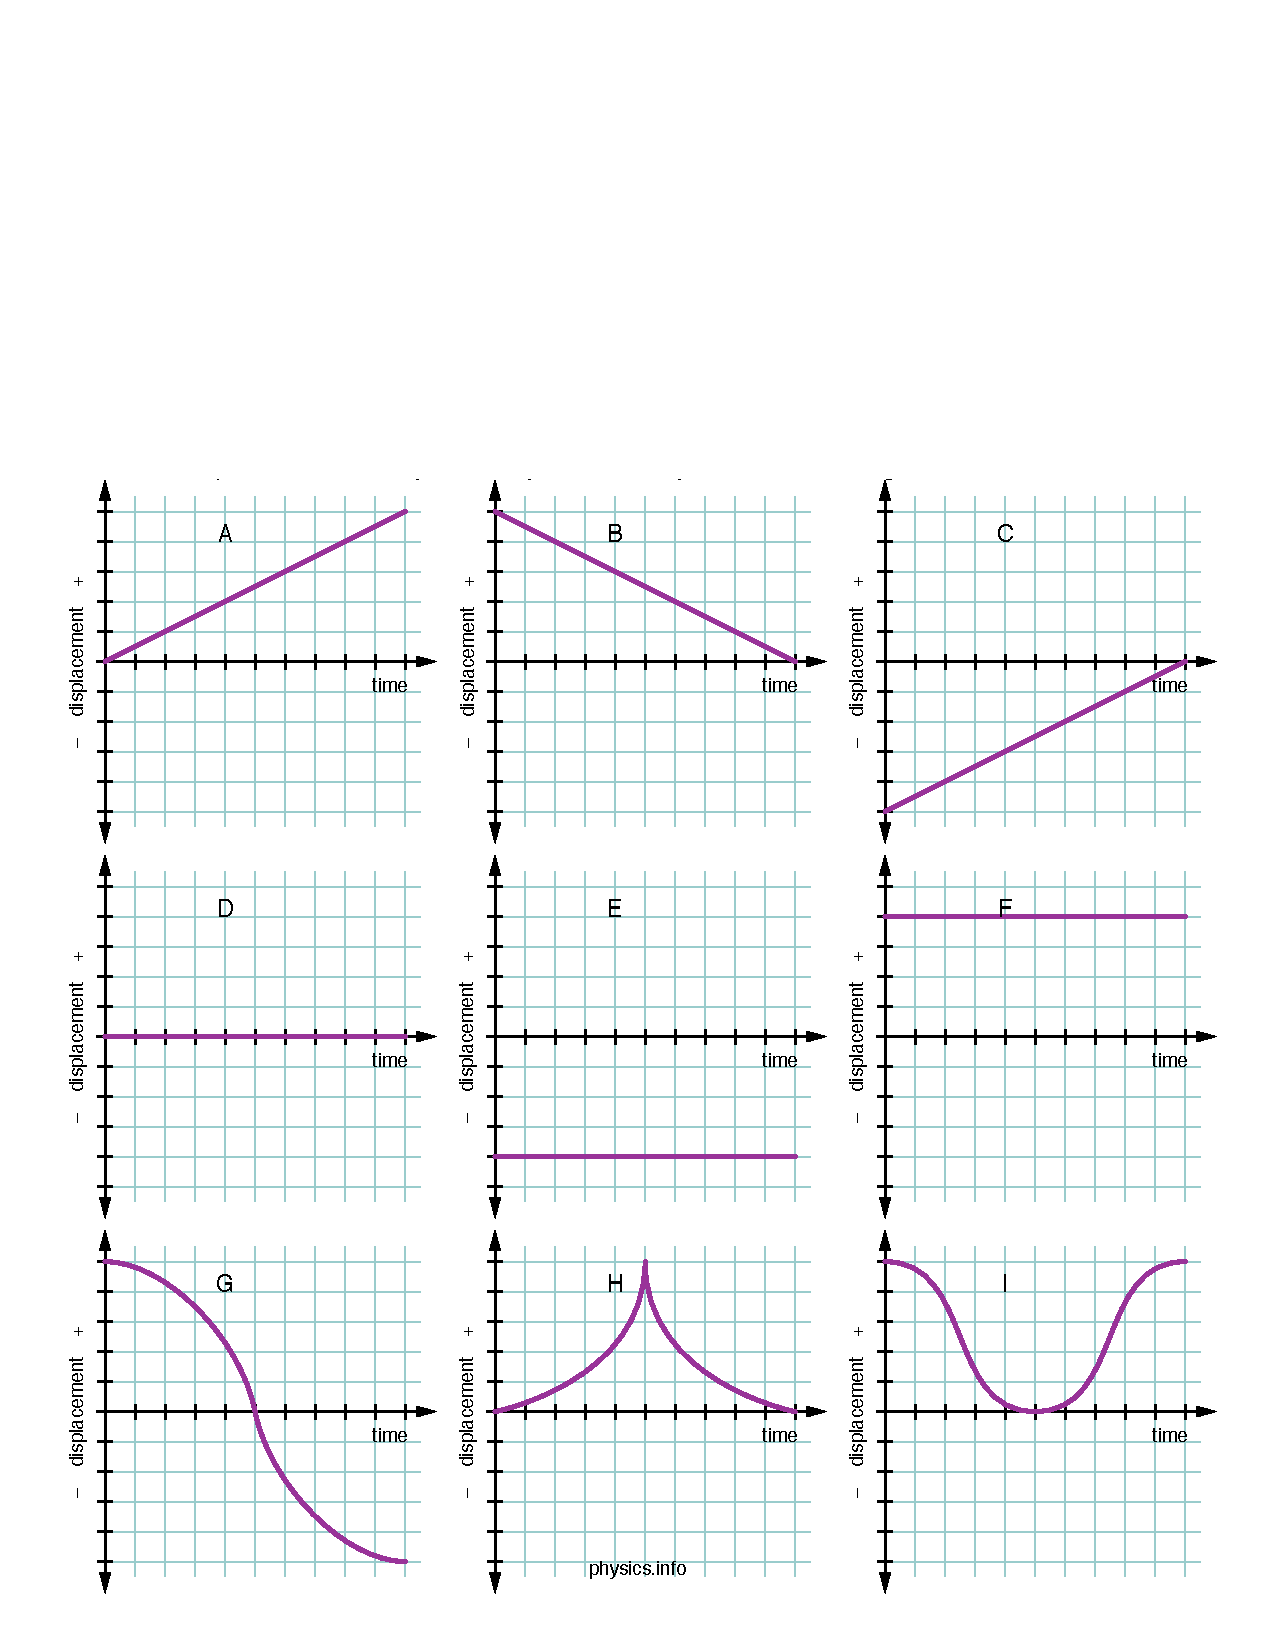
\includegraphics[width=0.8\textwidth]{choose-displacement.pdf}
    \caption{Linear motion displacement graphs.}
    \label{fig:descript}
\end{figure}














\section*{\textcolor{red}{Speed-time graphs. Rate of change of the speed.}}







\item Fill in the blanks: \cite{Nagwa} Q. 1 \href{https://www.nagwa.com/en/worksheets/257191315239/}{Lesson Worksheet: Speed–Time Graphs}\\
A \textbf{speed–time} graph shows the \textbf{change} in the  \underline{\hspace{3cm}} an object with \underline{\hspace{3cm}}.
%
\begin{itemize}
    %\item[A.] distance moved by, speed.
    \item[B.] speed of, time.
    \item[\textcolor{blue}{\bf B.}] \textcolor{blue}{\bf speed of, time.}
    \item[C.] speed of, distance moved.
    \item[D.] distance moved by, time.
\end{itemize}
%












\item Which of the following is a speed–time graph? \cite{Nagwa} Q. 2 \href{https://www.nagwa.com/en/worksheets/257191315239/}{Lesson Worksheet: Speed–Time Graphs}\\
%
\begin{figure}[H]
    \centering
    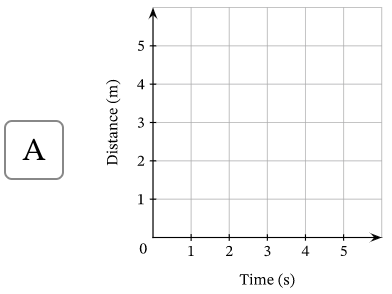
\includegraphics[width=0.35\textwidth]{Nagwa_Q1_Speedt-1.png}
    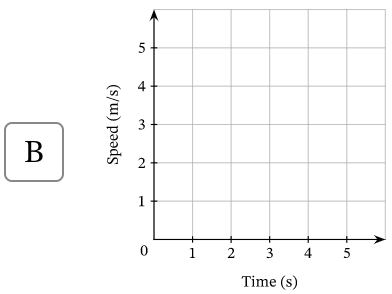
\includegraphics[width=0.35\textwidth]{Nagwa_Q1_Speedt-2.png}
\end{figure}
% \begin{solution}
% \begin{equation*}
%     \boxed{\text{\bf B}}
% \end{equation*}
% \end{solution}












\item \textbf{Which color} line shows the object that has the \textbf{greatest speed}? \cite{Nagwa} Q. 3 \href{https://www.nagwa.com/en/worksheets/257191315239/}{Lesson Worksheet: Speed–Time Graphs}
%
\begin{figure}[H]
    \centering
    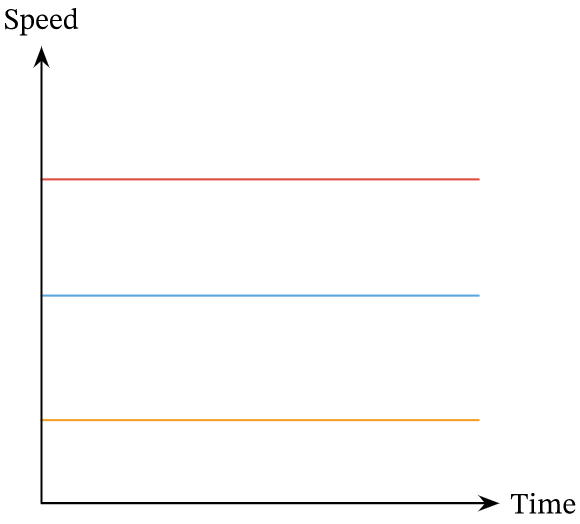
\includegraphics[width=0.4\textwidth]{Nagwa_Q3_Speedt.png}
\end{figure}
%
\begin{itemize}
    \item[A.] Blue
    \item[B.] Orange
    \item[C.] Red
    %\item[\textcolor{blue}{\bf C.}] \textcolor{blue}{\bf Red}
\end{itemize}
%










\item \textbf{Which color} line on the \textbf{speed–time graph} shows the motion of the object on the \textbf{distance–time} graph? \cite{Nagwa} Q. 4 \href{https://www.nagwa.com/en/worksheets/257191315239/}{Lesson Worksheet: Speed–Time Graphs}
%
\begin{figure}[H]
    \centering
    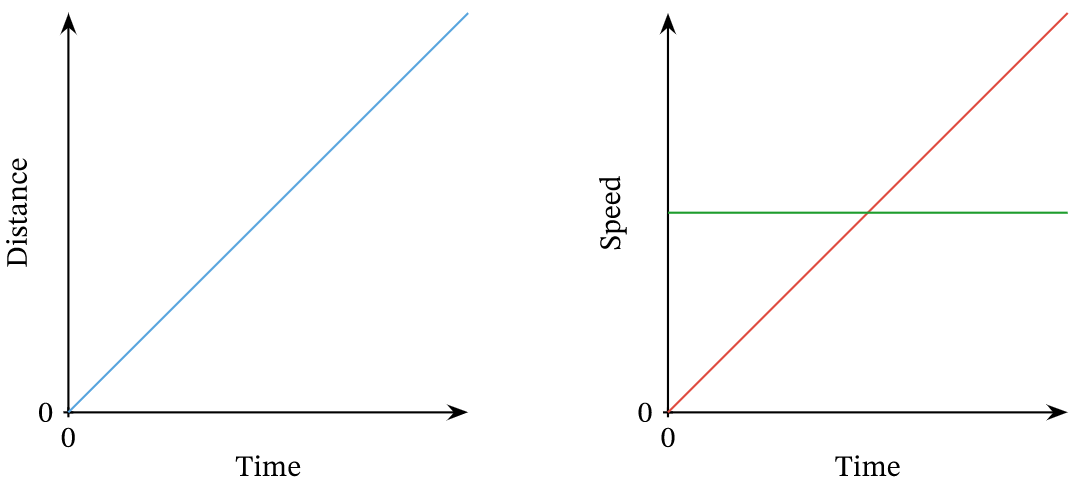
\includegraphics[width=0.7\textwidth]{Nagwa_Q4_Speedt.png}
\end{figure}
%
\begin{itemize}
    \item[A.] Red
    \item[B.] Green
    %\item[\textcolor{blue}{\bf B.}] \textcolor{blue}{\bf Green}
\end{itemize}
%









\item What is the \textbf{speed} shown by the \textbf{speed–time graph}? \cite{Nagwa} Q. 5 \href{https://www.nagwa.com/en/worksheets/257191315239/}{Lesson Worksheet: Speed–Time Graphs}
%
\begin{figure}[H]
    \centering
    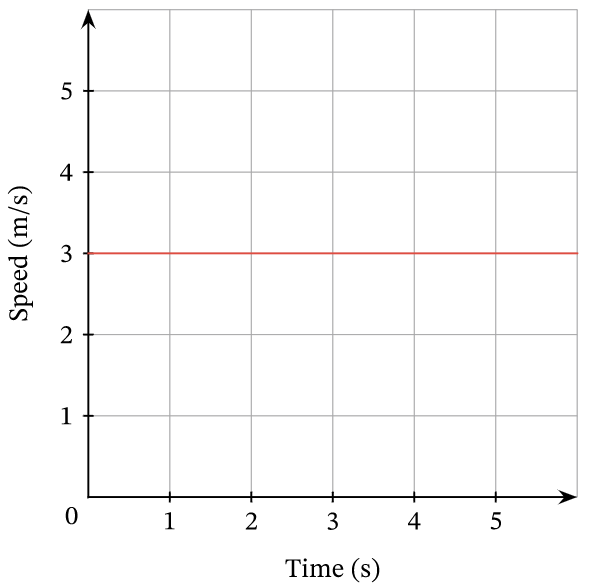
\includegraphics[width=0.4\textwidth]{Nagwa_Q5_Speedt.png}
\end{figure}
%
% \begin{solution}
% \begin{equation*}
%     \boxed{\text{\bf The speed is 3 m/s.}}
% \end{equation*}
% \end{solution}
%











\item \textbf{Which color} line on the \textbf{speed–time graph} shows the motion of the object on the \textbf{distance–time} graph? \cite{Nagwa} Q. 6 \href{https://www.nagwa.com/en/worksheets/257191315239/}{Lesson Worksheet: Speed–Time Graphs}
%
\begin{figure}[H]
    \centering
    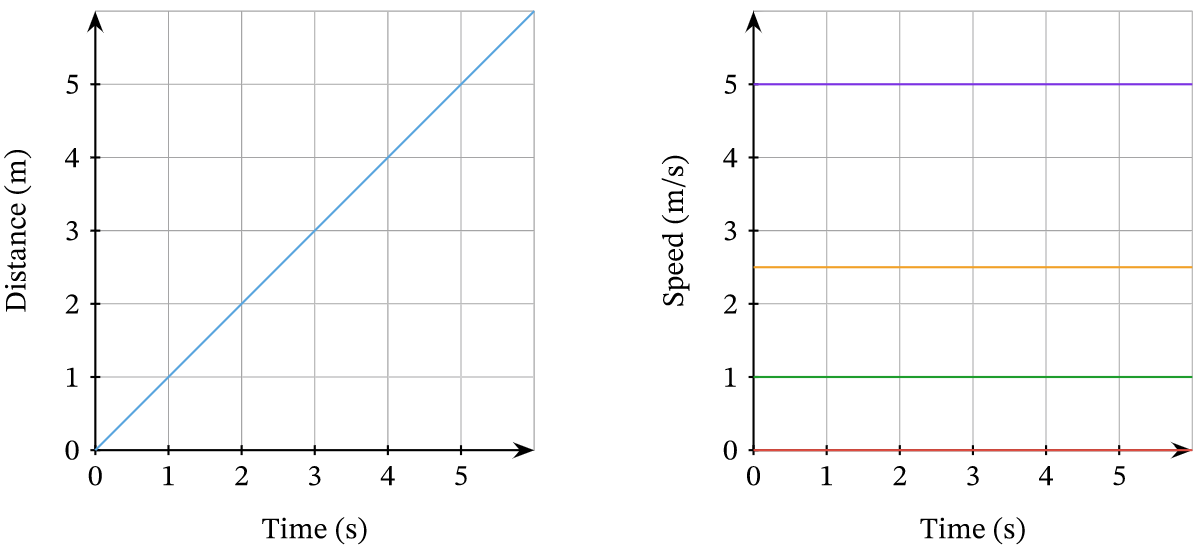
\includegraphics[width=0.7\textwidth]{Nagwa_Q6_Speedt.png}
\end{figure}
%
\begin{itemize}
    \item[A.] Orange
    \item[B.] Red
    \item[C.] Green
    \item[D.] Purple
\end{itemize}
%
% \begin{solution}
% The gradient of the \textbf{distance-time graph} is the speed. The gradient of the distance time graph is:
% \begin{equation*}
%     \text{Slope}=\frac{\msis{5}}{\tsis{5}}=\vsis{1}
% \end{equation*}
% Therefore the \textbf{speed-time graph} that corresponds to the \textbf{distance-time graph} is the one with speed 1 m/s. therefore:
% \begin{equation*}
%     \boxed{\text{Green}}
% \end{equation*}
% \end{solution}












\item \textbf{Which color} line on either \textbf{graph} shows the motion of the object with the \textbf{greatest speed}? \cite{Nagwa} Q. 7 \href{https://www.nagwa.com/en/worksheets/257191315239/}{Lesson Worksheet: Speed–Time Graphs}
%
\begin{figure}[H]
    \centering
    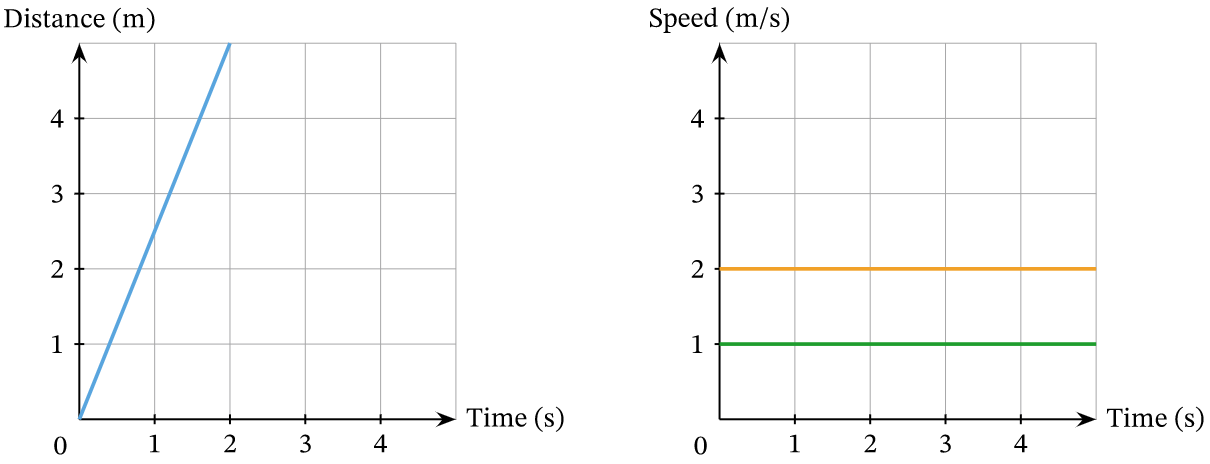
\includegraphics[width=0.8\textwidth]{Nagwa_Q7_Speedt.png}
\end{figure}
%
\begin{itemize}
    \item[A.] The blue line
    \item[B.] The orange line
    \item[C.] The green line
\end{itemize}
%
% \begin{solution}
% We are given three speeds with two different kinds of graphs.\\

% \textbf{Speed-time graph} gives the speed directly. In this case two speeds:\\
% $\vsis{1}$ and \vsis{2}.\\

% The third speed is given through the \textbf{distance-time graph}, therefore we need to calculate the slope to know the speed:
% \begin{equation*}
%     \text{Slope}=\text{Speed}=\frac{\text{Distance}}{\text{Time}}=\frac{\msis{5}}{\tsis{2}}=\vsis{2.5}
% \end{equation*}
% therefore,
% \begin{equation*}
%     \boxed{\text{The greatest speed is given by the blue line in the distance-time graph.}}
% \end{equation*}

% \end{solution}











\item \textbf{Which color} line on the \textbf{speed–time graph} shows the motion of the object on the \textbf{distance–time} graph? \cite{Nagwa} Q. 8 \href{https://www.nagwa.com/en/worksheets/257191315239/}{Lesson Worksheet: Speed–Time Graphs}
%
\begin{figure}[H]
    \centering
    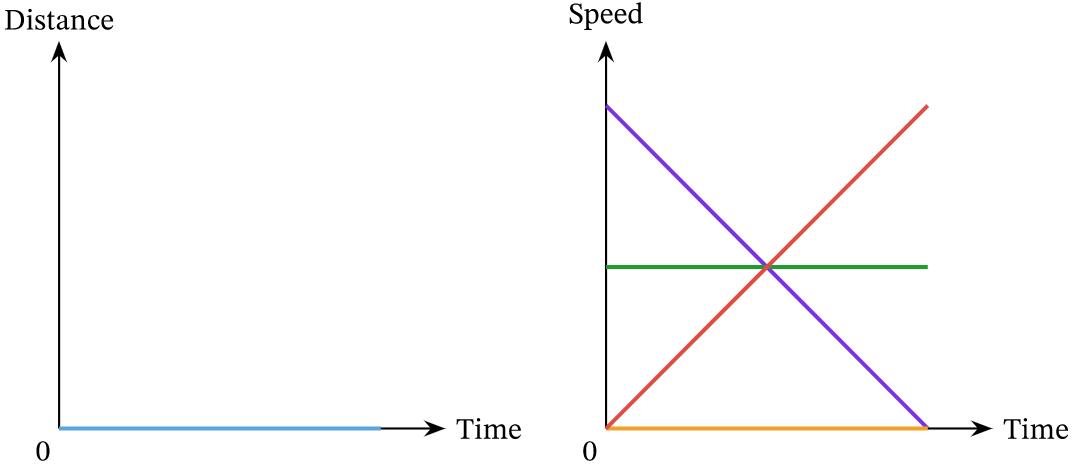
\includegraphics[width=0.8\textwidth]{Nagwa_Q8_Speedt.png}
\end{figure}
%
\begin{itemize}
    \item[A.] Orange
    \item[B.] Purple
    \item[C.] Red
    \item[D.] Green
\end{itemize}
%
% \begin{solution}
% The slope of the distance-time graph is always the speed of the motion. In this case the slope of the distance-time graph is clearly zero as the blue line is flat. In other words the distance does not change with time. This means that \textbf{the object is at rest}. If the object is at rest the speed must be necessarily ZERO. The graph describing zero speed in the \textbf{speed-time graph} is the ORANGE line.
% \begin{equation*}
%     \boxed{\text{The Orange line, speed$=0$.}}
% \end{equation*}
% \end{solution}
%













\item \textbf{Which} of the following is the name of the unit shown on the vertical axis of this graph?  \cite{Nagwa} Q. 9 \href{https://www.nagwa.com/en/worksheets/257191315239/}{Lesson Worksheet: Speed–Time Graphs}
%
\begin{figure}[H]
    \centering
    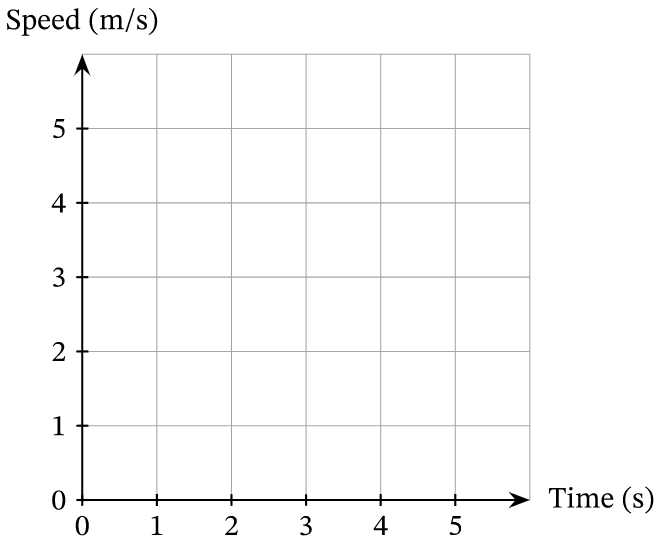
\includegraphics[width=0.4\textwidth]{Nagwa_Q9_Speedt.png}
\end{figure}
%
\begin{itemize}
    \item[A.] Seconds per meter
    \item[B.] Meter-seconds
    %\item[\textcolor{blue}{\bf B.}] \textcolor{blue}{\bf Meter-seconds}
    \item[C.] Meters per second per second
    \item[D.] Meters per second
    \item[E.] Seconds
\end{itemize}












\item Which of the following speed–time graphs is correct for an object that is not moving? \cite{Nagwa} Q. 10 \href{https://www.nagwa.com/en/worksheets/257191315239/}{Lesson Worksheet: Speed–Time Graphs}
%
\begin{figure}[H]
    \centering
    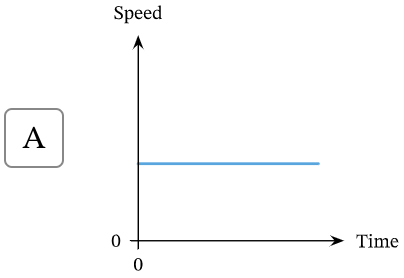
\includegraphics[width=0.4\textwidth]{Nagwa_Q10_Speedt-1.png} \hfill
    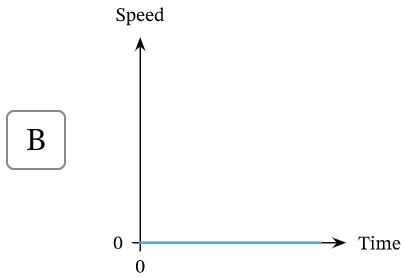
\includegraphics[width=0.4\textwidth]{Nagwa_Q10_Speedt-2.png}
\end{figure}
%
\begin{itemize}
    \item[A.] Only A.
    \item[B.] Only B.
    %\item[\textcolor{blue}{\bf B.}] \textcolor{blue}{\bf Only B.}
    \item[C.] Both graphs are correct for an object that is not moving.
\end{itemize}


\subsection*{\textcolor{red}{Speed-time graphs. Rate of change of speed.}}





\item This is a \textbf{speed-time} graph for a car moving between two sets of traffic lights. \cite{bbc, Triguero} \href{https://www.bbc.co.uk/bitesize/guides/znpp92p/revision/6}{*}
%
\begin{figure}[H]
    \centering
    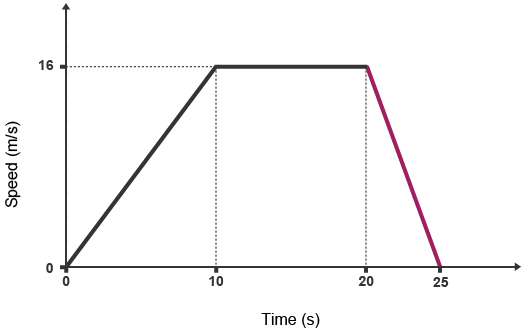
\includegraphics{bbc_rateofchangeSpeed.png}
    \caption{Caption}
    \label{fig:my_label}
\end{figure}
%
\begin{itemize}
    \item[\bf (a)] What is the \textbf{rate of change of speed} of the car between \textbf{0 s} and \textbf{10 s}? %1.6 m/s^2
    %
    \begin{example}
    The \textbf{rate of change of speed} is the \textbf{slope or gradient} of the \textbf{speed-time graph}.\\
    
    Rate of change of speed = gradient or slope of the speed-time graph.
    %
    \begin{equation*}
        \boxed{\text{Rate of change of speed}=\frac{\text{final speed}-\text{initial speed}}{\text{time taken}}=\frac{\vsis{16}-\vsis{0}}{\tsis{10}}=\asis{1.6}}
    \end{equation*}
    \end{example}
    %
    \item[\bf (b)] What is the \textbf{rate of change of speed} of the car between \textbf{10 s} and \textbf{20 s}?
    %
    % \begin{solution}
    % The \textbf{rate of change of speed} is the \textbf{slope or gradient} of the \textbf{speed-time graph}.\\
    
    % Rate of change of speed = gradient or slope of the speed-time graph.\\
    
    % No calculation is really needed as the line is horizontal and hence the slope is zero.
    
    % You can anyway do the calculation if you wish:
    % %
    % \begin{equation*}
    %     \boxed{\text{Rate of change of speed}=\frac{\text{final speed}-\text{initial speed}}{\text{time taken}}=\frac{\vsis{16}-\vsis{16}}{\tsis{10}}=\asis{0}}
    % \end{equation*}
    % \end{solution}
    %
    \item[\bf (c)] What is the \textbf{rate of change of speed} of the car between \textbf{20 s} and \textbf{25 s}? %-3.2 m/s^2
    %
    % \begin{solution}
    % The \textbf{rate of change of speed} is the \textbf{slope or gradient} of the \textbf{speed-time graph}.\\
    
    % Rate of change of speed = gradient or slope of the speed-time graph.
    % %
    % \begin{equation*}
    %     \boxed{\text{Rate of change of speed}=\frac{\text{final speed}-\text{initial speed}}{\text{time taken}}=\frac{\vsis{0}-\vsis{16}}{\tsis{5}}=\asis{-3.2}}
    % \end{equation*}
    % Notice that the rate of change of the speed is negative in this case.
    % \end{solution}
    %
\end{itemize}












\subsection*{\textcolor{red}{Speed-time graphs. Distance form speed time graphs}}











\item \textbf{Calculate} the \textbf{distance traveled} by a car between \textbf{0 s} and \textbf{10 s}, from its \textbf{speed-time} graph. \cite{Triguero}

\begin{figure}[H]
    \centering
    \begin{tikzpicture}
    \begin{axis}[clip=false,width=0.7\textwidth,height=0.4\textheight, xlabel={Time, $t$ [s]}, ylabel={Speed, $v$ [m/s]},
    xmin=0, xmax=11,
    ymin=0, ymax=4.5,
    xtick={0,1,2,3,4,5,6,7,8,9,10,11},
    ytick={0,1,2,3,4},
    legend pos=south east,
    grid=both,
    minor tick num=0]
    %
    %
    \addplot[name path=datitos,color=black,line width=1mm] coordinates {
	(0.00,4.0)
	(10.0,4.0)
    };
    \end{axis}
    \end{tikzpicture}
\end{figure}
%
%
\begin{example}
The speed time graph shows a movement with uniform (constant speed) of $\vsis{4}$. The distance travelled between $\tsis{0}$ and $\tsis{10}$ is the area below the graph between $\tsis{0}$ and $\tsis{10}$. In this case is just the area of the rectangle shown in the following graph:
\begin{figure}[H]
    \centering
    \begin{tikzpicture}
    \begin{axis}[clip=false,width=0.7\textwidth,height=0.6\textheight, xlabel={Time, $t$ [s]}, ylabel={Speed, $v$ [m/s]}]
    % Baseline
    \addplot[name path=baseline,white,domain=0:11] {5};
    % Baseline
    \addplot[name path=baseline,white,domain=0:10] {0};
    % Data
    \addplot[name path=datitos,color=red,line width=1mm] coordinates {
	(0.00,4.0)
	(10.0,4.0)
    };
    % Int
    \addplot[name path=int,color=red] coordinates {
	(0,4)
	(10,4)
    };
    % shade
    \addplot[red!15] fill between[of=baseline and int];
    \node[red] at (axis cs: 5,2) {\Huge\bf Distance};
    % arrows 1
    \draw[black,<->,line width=0.3mm] (axis cs: 10.25,0)--(axis cs: 10.25,4);
    \node[black,right] at (axis cs: 10.5,2) {\Large height};
    % arrows 1
    % base
    \draw[black,<->,line width=0.3mm] (axis cs: 0,4.25)--(axis cs: 10,4.25);
    \node[black] at (axis cs: 5,4.75) {\Large base};
    \end{axis}
    \end{tikzpicture}
\end{figure}
Base of the rectangle$=\msis{10}$\\
Height of the rectangle$=\vsis{4}$\\
Therefore, the distance is just the area of the rectangle,
\begin{equation*}
         \boxed{\text{Distance}=d=\text{base}\times\text{height}=\tsis{10}\times \vsis{4}=\msis{40}}
    \end{equation*}
\end{example}
%
















\item \textbf{Calculate} the \textbf{distance traveled} by a car between \textbf{0 s} and \textbf{15 s}, from its \textbf{speed-time} graph. \cite{Triguero}
\begin{figure}[H]
    \centering
    \begin{tikzpicture}
    \begin{axis}[width=0.7\textwidth,height=0.4\textheight, xlabel={time, $t$ [s]}, ylabel={speed, $v$ [m/s]},
    xmin=0, xmax=16,
    ymin=0, ymax=0.7,
    xtick={0,1,2,3,4,5,6,7,8,9,10,11,12,13,14,15,16},
    ytick={0,0.1,0.2,0.3,0.4,0.5,0.6,0.7},
    legend pos=south east,
    grid=both,
    minor tick num=0]
    %
    \addplot[name path=datitos,color=black,line width=1mm] coordinates {
	(0.00,0.0)
	(15.0,0.6)
    };
    \end{axis}
    \end{tikzpicture}
\end{figure}
%
\begin{example}
The speed-time graph shows a movement a growing speed (constant rate of change of speed) from $\vsis{0}$ to $\vsis{0.6}$. The distance travelled between $\tsis{0}$ and $\tsis{15}$ is the area below the graph between $\tsis{0}$ and $\tsis{15}$. In this case is just the area of the \textbf{triangle} shown in the following graph:
\begin{figure}[H]
    \centering
    \begin{tikzpicture}
    \begin{axis}[width=0.7\textwidth,height=0.6\textheight, xlabel={time, $t$ [s]}, ylabel={speed, $v$ [m/s]},
    xmin=0, xmax=20,
    ymin=0, ymax=0.8]
    % Baseline
    \addplot[name path=baseline,white,domain=0:15] {0};
    % Data
    \addplot[name path=datitos,color=red,line width=1mm] coordinates {
	(0.00,0.0)
	(15.0,0.6)
    };
    % Int
    \addplot[name path=int,color=red] coordinates {
	(0.0,0.0)
	(15.0,0.6)
    };
    % shade
    \addplot[red!15] fill between[of=baseline and int];
    \node[red] at (axis cs: 10,0.2) {\Huge\bf Distance};
    % arrows 1
    \draw[black,<->,line width=0.3mm] (axis cs: 16,0)--(axis cs: 16,0.6);
    \node[black,right] at (axis cs: 16,0.3) {\Large height};
    % base
    \draw[black,<->,line width=0.3mm] (axis cs: 0,0.65)--(axis cs: 15,0.65);
    \node[black] at (axis cs: 7.5,0.75) {\Large base};
    \end{axis}
    \end{tikzpicture}
    \end{figure}
    therefore,
    \begin{equation*}
         \boxed{d=\frac{1}{2}\,\text{base}\times\text{height}= \frac{1}{2}\times\tsis{15}\times \vsis{0.6}=\msis{4.5}}
    \end{equation*}
\end{example}
%





















\item \textbf{Calculate} the \textbf{distance traveled} by a car between the times \textbf{10 s} and \textbf{15 s}, from its \textbf{speed-time} graph. \cite{Triguero}
%
\begin{figure}[H]
    \centering
    \begin{tikzpicture}
    \begin{axis}[width=0.7\textwidth,height=0.4\textheight, xlabel={time, $t$ [s]}, ylabel={speed, $v$ [m/s]},
    xmin=0, xmax=22,
    ymin=0, ymax=0.9,
    xtick={0,1,2,3,4,5,6,7,8,9,10,11,12,13,14,15,16,17,18,19,20,21,22},
    ytick={0,0.1,0.2,0.3,0.4,0.5,0.6,0.7,0.8,0.9},
    legend pos=south east,
    grid=both,
    minor tick num=0
    ]
    % Data
    \addplot[name path=datitos,color=black,line width=1mm] coordinates {
	(0.00,0.0)
	(20.0,0.8)
    };
    \end{axis}
    \end{tikzpicture}
    \end{figure}
%
%
\begin{example}
In this case the \textbf{area under the graph} is not as simple as in previous problems. In this case we can decompose the total area shape into simpler shapes. In particular, we can calculate the area of the figure considering one \textbf{triangle} and one \textbf{rectangle}.\\

The area of the rectangle $=$ base$\times$ height$_1$\\

The area of the triangle $=\frac{1}{2}$ base$\times$ height$_2$\\

Adding the area of these two figures we obtain the distance.
%
\begin{figure}[H]
    \centering
    \begin{tikzpicture}
    \begin{axis}[width=0.7\textwidth,height=0.6\textheight, xlabel={time, $t$ [s]}, ylabel={speed, $v$ [m/s]},
    xmin=0, xmax=22,
    ymin=0, ymax=0.9,
    xtick={0,1,2,3,4,5,6,7,8,9,10,11,12,13,14,15,16,17,18,19,20,21,22},
    ytick={0,0.1,0.2,0.3,0.4,0.5,0.6,0.7,0.8,0.9},
    legend pos=south east,
    grid=both,
    minor tick num=0
    ]
    % Baseline
    \addplot[name path=baseline,white,domain=10:15] {0};
    % separation
    \addplot[name path=sep,white,dashed,domain=10:15,line width=0.3mm] {0.4};
    % Data
    \addplot[name path=datitos,color=red,line width=1mm] coordinates {
	(0.00,0.0)
	(20.0,0.8)
    };
    % Int
    \addplot[name path=int,color=red] coordinates {
	(10.0,0.4)
	(15.0,0.6)
    };
    % shade
    \addplot[red!15] fill between[of=baseline and int];
    \node[white] at (axis cs: 12.5,0.225) {\large\bf distance};
    % arrows 1
    \draw[black,<->,line width=0.3mm] (axis cs: 16,0)--(axis cs: 16,0.4);
    \node[black,right] at (axis cs: 16,0.2) {\Large height$_1$};
    % arrows 1
    \draw[black,<->,line width=0.3mm] (axis cs: 16,0.4)--(axis cs: 16,0.6);
    \node[black,right] at (axis cs: 16,0.5) {\Large height$_2$};
    % base
    \draw[black,<->,line width=0.3mm] (axis cs: 10,0.65)--(axis cs: 15,0.65);
    \node[black] at (axis cs: 12.5,0.75) {\Large base};
    \end{axis}
    \end{tikzpicture}
    \end{figure}
    
    \begin{equation*}
    \begin{split}
         & d=\text{base}\times\text{height}_1+ \frac{1}{2}\, \text{base}\times\text{height}_2\\
         & d= \tsis{5}\times \vsis{0.4}+\tsis{5}\times \vsis{0.2}=\msis{3}
    \end{split}
    \end{equation*}
\end{example}
%












\item The figure below shows the speed-time graph of an object. \cite{Triguero}
\begin{figure}[H]
    \centering
    \begin{tikzpicture}
    \begin{axis}[width=0.7\textwidth,height=0.4\textheight, xlabel={time, $t$ [s]}, ylabel={speed, $v$ [m/s]},
    xmin=0, xmax=25,
    ymin=0, ymax=20,
    xtick={0,1,2,3,4,5,6,7,8,9,10,11,12,13,14,15,16,17,18,19,20,21,22,23,24,25},
    ytick={0,1,2,3,4,5,6,7,8,9,10,11,12,13,14,15,16,17,18,19,20,21,22},
    legend pos=south east,
    grid=both,
    minor tick num=0
    ]
    % Data
    \addplot[name path=datitos,color=black,line width=1mm] coordinates {
	(0,0) (7,12) (11,12) (16,18)(19,18)(25,0)
    };
    \end{axis}
    \end{tikzpicture}
    \end{figure}
    %
\begin{itemize}
    \item[\bf (a)] Calculate the \textbf{distance} travelled from time \textbf{0 s} to time \textbf{7 s}.
    %
    %
%     \begin{solution}
%     \begin{figure}[H]
%     \centering
%     \begin{tikzpicture}
%     \begin{axis}[width=0.7\textwidth,height=0.4\textheight, xlabel={time, $t$ [s]}, ylabel={speed, $v$ [m/s]},
%     xmin=0, xmax=25,
%     ymin=0, ymax=20,
%     xtick={0,1,2,3,4,5,6,7,8,9,10,11,12,13,14,15,16,17,18,19,20,21,22,23,24,25},
%     ytick={0,1,2,3,4,5,6,7,8,9,10,11,12,13,14,15,16,17,18,19,20,21,22},
%     legend pos=south east,
%     grid=both,
%     minor tick num=0
%     ]
%     % Baseline
%     \addplot[name path=baseline,white,domain=0:7] {0};
%     % Int
%     \addplot[name path=int,color=red] coordinates {(0,0) (7,12)};
%     % Data
%     \addplot[name path=datitos,color=black,line width=1mm] coordinates {
% 	(0,0) (7,12) (11,12) (16,18)(19,18)(25,0)
%     };
%     % shade
%     \addplot[red!50] fill between[of=baseline and int];
%     \node[white] at (axis cs: 4,2) {\large\bf Distance};
%     \end{axis}
%     \end{tikzpicture}
%     \end{figure}
%     %
%     \begin{equation*}
%         \boxed{\text{Distance}=\frac{1}{2}\text{base}\times\text{height}=\frac{1}{2}\cdot\tsis{7}\cdot\vsis{12}=\msis{42}}
%     \end{equation*}
%     \end{solution}
    %
    \item[\bf (b)] Calculate the \textbf{distance} travelled from time \textbf{19 s} to time \textbf{25 s}.
    %
    %
%     \begin{solution}
%     \begin{figure}[H]
%     \centering
%     \begin{tikzpicture}
%     \begin{axis}[width=0.7\textwidth,height=0.4\textheight, xlabel={time, $t$ [s]}, ylabel={speed, $v$ [m/s]},
%     xmin=0, xmax=25,
%     ymin=0, ymax=20,
%     xtick={0,1,2,3,4,5,6,7,8,9,10,11,12,13,14,15,16,17,18,19,20,21,22,23,24,25},
%     ytick={0,1,2,3,4,5,6,7,8,9,10,11,12,13,14,15,16,17,18,19,20,21,22},
%     legend pos=south east,
%     grid=both,
%     minor tick num=0
%     ]
%     % Baseline
%     \addplot[name path=baseline,white,domain=19:25] {0};
%     % Int
%     \addplot[name path=int,color=red] coordinates {(19,18)(25,0)};
%     % Data
%     \addplot[name path=datitos,color=black,line width=1mm] coordinates {
% 	(0,0) (7,12) (11,12) (16,18)(19,18)(25,0)
%     };
%     % shade
%     \addplot[red!50] fill between[of=baseline and int];
%     \node[white] at (axis cs: 22,1) {\large\bf Distance};
%     \end{axis}
%     \end{tikzpicture}
%     \end{figure}
%     %
%     \textbf{Area from 19 s to 25 s:}
%     \begin{equation*}
%         \boxed{\text{Distance}=\frac{1}{2}\text{base}\times\text{height}=\frac{1}{2}\cdot\tsis{(25-19)}\cdot\vsis{18}=\msis{54}}
%     \end{equation*}
%     \end{solution}
    %
    \item[\bf (c)] Calculate the \textbf{distance} travelled from time \textbf{7 s} to time \textbf{19 s}.
    %
    %
%     \begin{solution}
%     \begin{figure}[H]
%     \centering
%     \begin{tikzpicture}
%     \begin{axis}[width=0.7\textwidth,height=0.4\textheight, xlabel={time, $t$ [s]}, ylabel={speed, $v$ [m/s]},
%     xmin=0, xmax=25,
%     ymin=0, ymax=20,
%     xtick={0,1,2,3,4,5,6,7,8,9,10,11,12,13,14,15,16,17,18,19,20,21,22,23,24,25},
%     ytick={0,1,2,3,4,5,6,7,8,9,10,11,12,13,14,15,16,17,18,19,20,21,22},
%     legend pos=south east,
%     grid=both,
%     minor tick num=0
%     ]
%     % Baseline
%     \addplot[name path=baseline,white,domain=7:19] {0};
%     % Int
%     \addplot[name path=int,color=red] coordinates {(7,12) (11,12) (16,18)(19,18)};
%     % Data
%     \addplot[name path=datitos,color=black,line width=1mm] coordinates {
% 	(0,0) (7,12) (11,12) (16,18)(19,18)(25,0)
%     };
%     % shade
%     \addplot[red!50] fill between[of=baseline and int];
%     % Guide lines for figures
%     % First rectangle
%     \draw[dashed, black] (axis cs: 7,0) -- (axis cs: 7,12);
%     \draw[dashed, black] (axis cs: 11,0) -- (axis cs: 11,12);
%     % second rectangle
%     \draw[dashed, black] (axis cs: 11,0) -- (axis cs: 11,12)--(axis cs: 16,12)--(axis cs: 16,0);
%     % triangle
%     \draw[dashed, black] (axis cs: 16,12) -- (axis cs: 16,18);
%     % last rectangle
%     \draw[dashed, black] (axis cs: 19,0) -- (axis cs: 19,18);
%     %
%     \node[white] at (axis cs: 13,7) {\large\bf Distance};
%     \end{axis}
%     \end{tikzpicture}
%     \end{figure}
%     %
%     \textbf{Area from 7 s to 11 s:}
%     \begin{equation*}
%         \text{Distance}=\text{base}\times\text{height}=\cdot\tsis{(11-7)}\cdot\vsis{12}=\msis{48}
%     \end{equation*}
%     %
%     \textbf{Area from 11 s to 16 s:}
%     \begin{equation*}
%     \begin{split}
%         & \text{Distance}=\text{base}\times\text{height}_1+\frac{1}{2}\text{base}\times\text{height}_2=\\
%         & \tsis{(16-11)}\cdot\vsis{(12-0)}+
%         \frac{1}{2}\cdot\tsis{(16-11)}\cdot\vsis{(18-12)}=\\
%         & \msis{60}+\msis{15}=\msis{75}
%         \end{split}
%     \end{equation*}
%         %
%     \textbf{Area from 16 s to 19 s:}
%     \begin{equation*}
%     \begin{split}
%         & \text{Distance}=\text{base}\times\text{height}=\tsis{(19-16)}\cdot\vsis{(18-0)}=\msis{54}
%         \end{split}
%     \end{equation*}
%     therefore, the distance travelled from 7 s to 19 s is the sum of the intervals,
%     \begin{equation*}
%         \boxed{\text{Distance}=\msis{48}+\msis{75}+\msis{54}=\msis{177}}
%     \end{equation*}
%     \end{solution}
%     %
    \item[\bf (d)] Calculate the \textbf{distance} travelled from time \textbf{9 s} to time \textbf{14 s}.
%     %
%     %
%     \begin{solution}
%     \begin{figure}[H]
%     \centering
%     \begin{tikzpicture}
%     \begin{axis}[width=0.7\textwidth,height=0.4\textheight, xlabel={time, $t$ [s]}, ylabel={speed, $v$ [m/s]},
%     xmin=0, xmax=25,
%     ymin=0, ymax=20,
%     xtick={0,1,2,3,4,5,6,7,8,9,10,11,12,13,14,15,16,17,18,19,20,21,22,23,24,25},
%     ytick={0,1,2,3,4,5,6,7,8,9,10,11,12,13,14,15,16,17,18,19,20,21,22},
%     legend pos=south east,
%     grid=both,
%     minor tick num=0
%     ]
%     % Baseline
%     \addplot[name path=baseline,white,domain=9:14] {0};
%     % Int
%     \addplot[name path=int,color=red] coordinates {(9,12) (11,12) (14,15.6)};
%     % Data
%     \addplot[name path=datitos,color=black,line width=1mm] coordinates {
% 	(0,0) (7,12) (11,12) (16,18)(19,18)(25,0)
%     };
%     % shade
%     \addplot[red!50] fill between[of=baseline and int];
%     \node[white] at (axis cs: 22,1) {\large\bf Distance};
%     \end{axis}
%     \end{tikzpicture}
%     \end{figure}
%     %
%     \textbf{Area from 9 s to 11 s:}
%     \begin{equation*}
%         \text{Distance}=\text{base}\times\text{height}=\cdot\tsis{(11-9)}\cdot\vsis{12}=\msis{24}
%     \end{equation*}
%     %
%     \textbf{Area from 11 s to 14 s:}
%     \begin{equation*}
%     \begin{split}
%         & \text{Distance}=\text{base}\times\text{height}_1+\frac{1}{2}\text{base}\times\text{height}_2=\\
%         & \tsis{(14-11)}\cdot\vsis{(12-0)}+
%         \frac{1}{2}\cdot\tsis{(14-11)}\cdot\vsis{(15.6-12)}=\\
%         & \msis{36}+\msis{5.4}=\msis{41.4}
%         \end{split}
%     \end{equation*}
%     %
%     therefore, the distance travelled from 7 s to 19 s is the sum of the intervals,
%     \begin{equation*}
%         \boxed{\text{Distance}=\msis{24}+\msis{41.4}=\msis{65.4}}
%     \end{equation*}
%     You can just consider 1 rectangle and one triangle...
%     \end{solution}
    %
    \item[\bf (e)] Calculate the \textbf{total distance} travelled in the whole interval.
    %
    % \begin{solution}
    % The total distance is the sum of the distances calculated in sections \textbf{(a)}, \textbf{(b)}, and \textbf{(c)}.
    % \begin{equation*}
    %     \boxed{\text{Total distance}=\msis{42}+\msis{177}+\msis{54}=\msis{273}}
    % \end{equation*}
    % To solve every section you could have count the squares too!!!
    % \end{solution}
    
    %
\end{itemize}





\subsection*{\textcolor{red}{Speed-time graphs. Average speed.}}




\section*{\textcolor{red}{Velocity-time graphs. Acceleration.}}


\item {\it Extracting the 3 main pieces of information from a velocity-time graph and beyond.}\\

Consider the following \textbf{velocity-time} graph:

\begin{figure}[H]
    \centering
    \begin{tikzpicture}
    \begin{axis}[width=0.7\textwidth,height=0.4\textheight, xlabel={time, $t$ [s]}, ylabel={velocity, $v$ [m/s]},
    xmin=0, xmax=20,
    ymin=-6, ymax=10,
    xtick={0,1,2,3,4,5,6,7,8,9,10,11,12,13,14,15,16,17,18,19,20,21,22,23,24,25},
    ytick={-6,-5,-4,-3,-2,-1,0,1,2,3,4,5,6,7,8,9,10},
    legend pos=south east,
    grid=both,
    minor tick num=0
    ]
    % Data
    \addplot[name path=datitos,color=black,line width=1mm] coordinates {
	(0,0) (4,8) (7,8) (10,-4)(16,0)(20,0)
    };
    % % Baseline
    % \addplot[name path=baseline,white,domain=9:14] {0};
    % % Int
    % \addplot[name path=int,color=red] coordinates {(9,12) (11,12) (14,15.6)};
    % % shade
    % \addplot[red!50] fill between[of=baseline and int];
    % \node[white] at (axis cs: 22,1) {\large\bf Distance};
    \end{axis}
    \end{tikzpicture}
    \end{figure}
\begin{itemize}
    \item[] {\bf Velocity from velocity-time graphs:}
    \item[\bf (a)] At what time or time interval the object \textbf{velocity} was \textbf{greatest}?
    %
    \begin{example}
    The greatest velocity was achieved in the interval 4 s to 7 s.
    
    \begin{equation*}
      \boxed{\text{Greatest velocity was achieved between }t=\tsis{4}\text{ and }t=\tsis{7}}
    \end{equation*}
    \end{example}
    %
    \item[\bf (b)] At what times or time intervals the object was at \textbf{rest} (zero velocity)?
    %
    \begin{example}
    In a distance-time or displacement-time graph rest means zero slope.
    
    In a \textbf{speed-time} or \textbf{velocity-time} graph \textbf{rest means} that the \textbf{value is zero}.
    
    \begin{equation*}
        \boxed{\text{The object is at rest at: } \tsis{t=0},\,\,\tsis{t=9}\text{, and over the interval from }t=\tsis{16}\text{ until } t=\tsis{20}}
    \end{equation*}
    \end{example}
    %
    \item[] {\bf Acceleration from velocity-time graphs:}
    \item[\bf (c)] Calculate the \textbf{acceleration} over the interval \textbf{0 s} to \textbf{4 s}.
    %
    \begin{example}
    The acceleration is the slope of the graph.
    \begin{equation*}
       \boxed{a=\frac{v_\text{f}-v_\text{i}}{t_\text{f}-t_\text{i}}=\frac{\vsis{8}-\vsis{0}}{\tsis{4}-\tsis{0}}=\asis{+2}}
    \end{equation*}
    \end{example}
    %
    \item[\bf (d)] Calculate the \textbf{acceleration} over the interval \textbf{10 s} to \textbf{16 s}.
    %
    \begin{example}
    The acceleration is the slope of the graph.
    \begin{equation*}
       \boxed{a=\frac{v_\text{f}-v_\text{i}}{t_\text{f}-t_\text{i}}=\frac{\vsis{0}-(\vsis{-4})}{\tsis{16}-\tsis{10}}=\asis{+0.67}}
    \end{equation*}
    \end{example}
    %
    \item[\bf (e)] Calculate the \textbf{acceleration} over the interval \textbf{7 s} to \textbf{10 s}.
    %
    \begin{example}
    The acceleration is the slope of the graph.
    \begin{equation*}
       \boxed{a=\frac{v_\text{f}-v_\text{i}}{t_\text{f}-t_\text{i}}=\frac{(\vsis{-4})-\vsis{8}}{\tsis{10}-\tsis{7}}=\frac{(\vsis{-12})}{\tsis{3}}=\asis{-4}}
    \end{equation*}
    \end{example}
    %
    \item[] {\bf Displacement from velocity-time graphs:}
    \item[\bf (f)] Calculate the \textbf{displacement} over the first \textbf{9 s}.
    %
    \begin{example}
    This is exactly as we did for the speed as the velocity is positive. We need to calculate the area under the graph in the given interval.
    
    \begin{figure}[H]
    \centering
    \begin{tikzpicture}
    \begin{axis}[width=0.7\textwidth,height=0.4\textheight, xlabel={time, $t$ [s]}, ylabel={velocity, $v$ [m/s]},
    xmin=0, xmax=20,
    ymin=-6, ymax=10,
    xtick={0,1,2,3,4,5,6,7,8,9,10,11,12,13,14,15,16,17,18,19,20,21,22,23,24,25},
    ytick={-6,-5,-4,-3,-2,-1,0,1,2,3,4,5,6,7,8,9,10},
    legend pos=south east,
    grid=both,
    minor tick num=0
    ]
    % Data
    \addplot[name path=datitos,color=black,line width=1mm] coordinates {
	(0,0) (4,8) (7,8) (10,-4)(16,0)(20,0)
    };
    % Baseline
    \addplot[name path=baseline,white,domain=0:9] {0};
    % Int
    \addplot[name path=int,color=red] coordinates {(0,0) (4,8) (7,8)};
    % shade
    \addplot[red!50] fill between[of=baseline and int];
    \node[white] at (axis cs: 22,1) {\large\bf Displacement};
    % Figures to consider
    \draw[dashed,black] (axis cs: 4,0)--(axis cs: 4,8);
    \draw[dashed,black] (axis cs: 7,0)--(axis cs: 7,8);
    \draw[dashed,black] (axis cs: 0,0)--(axis cs: 9,0);
    \end{axis}
    \end{tikzpicture}
    \end{figure}
    In practice we need to calculate the area of the two triangles and the square.\\
    
    {Area of interval 0 s to 4 s:}
    \begin{equation*}
       \text{Displacement}=\text{Area}=\frac{1}{2}\cdot \text{base}\times\text{height}=\frac{1}{2}\cdot\tsis{4}\times\vsis{8}=\msis{+16}
    \end{equation*}
    {Area of interval 4 s to 7 s:}
    \begin{equation*}
      \text{Displacement}=\text{Area}= \text{base}\times\text{height}=\tsis{3}\times\vsis{8}=\msis{+24}
    \end{equation*}
        {Area of interval 7 s to 9 s:}
    \begin{equation*}
       \text{Displacement}=\text{Area}=\frac{1}{2}\cdot \text{base}\times\text{height}=\frac{1}{2}\cdot\tsis{2}\times\vsis{8}=\msis{+8}
    \end{equation*}
    therefore,
    \begin{equation*}
        \boxed{\text{Displacement}=\msis{+16}+\msis{+24}+\msis{+8}=\msis{48}}
    \end{equation*}
    \end{example}
    %
    \item[\bf (g)] Calculate the \textbf{displacement} over the first \textbf{16 s}.
    %
    \begin{example}
    From 0 s to 9 s the result is the same as the calculated in the previous section. From 9 s to 16 s the contribution to the displacement is negative because the velocity is negative in that interval.
     \begin{figure}[H]
    \centering
    \begin{tikzpicture}
    \begin{axis}[width=0.7\textwidth,height=0.4\textheight, xlabel={time, $t$ [s]}, ylabel={velocity, $v$ [m/s]},
    xmin=0, xmax=20,
    ymin=-6, ymax=10,
    xtick={0,1,2,3,4,5,6,7,8,9,10,11,12,13,14,15,16,17,18,19,20,21,22,23,24,25},
    ytick={-6,-5,-4,-3,-2,-1,0,1,2,3,4,5,6,7,8,9,10},
    legend pos=south east,
    grid=both,
    minor tick num=0
    ]
    % Data
    \addplot[name path=datitos,color=black,line width=1mm] coordinates {
	(0,0) (4,8) (7,8) (10,-4)(16,0)(20,0)
    };
    % Baseline 1
    \addplot[name path=baseline1,white,domain=0:9] {0};
    % Baseline 2
    \addplot[name path=baseline2,white,domain=9:16] {0};
    % Int 1
    \addplot[name path=int1,color=red] coordinates {(0,0) (4,8) (7,8) (9,0)};
    % Int 2
    \addplot[name path=int2,color=red] coordinates {(9,0) (10,-4) (16,0)};
    % shade
    \addplot[red!50] fill between[of=baseline1 and int1];
    \addplot[blue!50] fill between[of=baseline2 and int2];
    \node[white] at (axis cs: 22,1) {\large\bf Displacement};
    % Figures to consider
    \draw[dashed,black] (axis cs: 4,0)--(axis cs: 4,8);
    \draw[dashed,black] (axis cs: 7,0)--(axis cs: 7,8);
    \draw[dashed,black] (axis cs: 0,0)--(axis cs: 9,0);
    \end{axis}
    \end{tikzpicture}
    \end{figure}
    %
    {\bf Area of interval 9 s to 10 s:}
    \begin{equation*}
       \text{Displacement}=\text{Area}=\frac{1}{2}\cdot \text{base}\times\text{height}=\frac{1}{2}\cdot\tsis{1}\times(\vsis{-4})=\msis{-2}
    \end{equation*}
    %
    {\bf Area of interval 10 s to 16 s:}
    \begin{equation*}
       \text{Displacement}=\text{Area}=\frac{1}{2}\cdot \text{base}\times\text{height}=\frac{1}{2}\cdot\tsis{6}\times(\vsis{-4})=\msis{-12}
    \end{equation*}
    therefore,
    \begin{equation*}
       \boxed{\text{Displacement}=\msis{48}-\msis{2}-\msis{12}=\msis{+34}}
    \end{equation*}
    \end{example}
    %
\end{itemize}
    















\item {\it About acceleration from velocity time graphs:} The change in \textbf{velocity} of an object over a \textbf{4-second} time interval is shown in the graph. What is the \textbf{acceleration} of the object? \cite{Nagwa} Q. 6, Q. 10 \href{https://www.nagwa.com/en/worksheets/684146965834/}{Lesson Worksheet: Acceleration over Time}
%
\begin{figure}[H]
    \centering
    \includegraphics{Nagwa_Q6_acel.png}
\end{figure}
%
% \begin{solution}
% The velocity increases uniformly from 0 s to 4 s. The sole of the graph is constant from 0 s to 4 s. The slope of the graph is the acceleration, therefore, the acceleration is constant.
% %
% \begin{equation*}
%     \boxed{a=\frac{v_\text{f}-v_\text{i}}{t_\text{f}-t_\text{i}}=\frac{\vsis{6}-\vsis{0}}{\tsis{4}-\tsis{0}}=\asis{\frac{3}{2}}=\asis{1.5}}
% \end{equation*}
% %
% \end{solution}
















\item The velocity-time graph shows the change in the velocity of a person walking in the time interval from $t=0$ s to $t=6$ s. The person’s starting point is their position when $t=0$ s.
%
% \begin{figure}[H]
%     \centering
%     \includegraphics[scale=0.8]{Nagwa_Q10_Velt.png}
% \end{figure}
%
\begin{figure}[H]
    \centering
    \begin{tikzpicture}
    \begin{axis}[width=0.7\textwidth,height=0.4\textheight, xlabel={time, $t$ [s]}, ylabel={velocity, $v$ [m/s]},
    xmin=0, xmax=6,
    ymin=-4, ymax=4,
    xtick={0,1,2,3,4,5,6},
    ytick={-4,-3,-2,-1,0,1,2,3,4},
    legend pos=south east,
    grid=both,
    minor tick num=0
    ]
    % Data
    \addplot[name path=datitos,color=black,line width=1mm] coordinates {
	(0,3) (2,3) (4,-3) (6,-3)};
    % % Baseline
    % \addplot[name path=baseline,white,domain=9:14] {0};
    % % Int
    % \addplot[name path=int,color=red] coordinates {(9,12) (11,12) (14,15.6)};
    % % shade
    % \addplot[red!50] fill between[of=baseline and int];
    % \node[white] at (axis cs: 22,1) {\large\bf Distance};
    \end{axis}
    \end{tikzpicture}
    \end{figure}
    %
\begin{itemize}
    \item[\bf (a)] What is the person’s \textbf{displacement} from their starting point after \textbf{2 seconds}?
    %
%     \begin{solution}
%     The person's displacement is the area under the graph from 0 s to 2 s.
%     %
% \begin{figure}[H]
%     \centering
%     \begin{tikzpicture}
%     \begin{axis}[width=0.7\textwidth,height=0.4\textheight, xlabel={time, $t$ [s]}, ylabel={velocity, $v$ [m/s]},
%     xmin=0, xmax=6,
%     ymin=-4, ymax=4,
%     xtick={0,1,2,3,4,5,6},
%     ytick={-4,-3,-2,-1,0,1,2,3,4},
%     legend pos=south east,
%     grid=both,
%     minor tick num=0
%     ]
%     % Data
%     \addplot[name path=datitos,color=black,line width=1mm] coordinates {
% 	(0,3) (2,3) (4,-3) (6,-3)};
%     % % Baseline
%     \addplot[name path=baseline,white,domain=0:2] {0};
%     % % Int
%     \addplot[name path=int,color=red] coordinates {(0,3) (2,3)};
%     % % shade
%     \addplot[red!50] fill between[of=baseline and int];
%     \node[white] at (axis cs: 1,1.5) {\large\bf Displacement};
%     \end{axis}
%     \end{tikzpicture}
%     \end{figure}
%     %
%     In this case is just the area of a rectangle of base 2 s and height 6 m/s.
%     %
%     \begin{equation*}
%         \boxed{\text{Displacement between 0 s and 2 s}=\text{base}\times\text{height}=\tsis{2}\times(\vsis{3}-\vsis{0})=\msis{6}}
%     \end{equation*}
%     %
%     \end{solution}
    %
    \item[\bf (b)] What is the person’s \textbf{displacement} from their starting point after \textbf{3 seconds}?
    %
%     \begin{solution}
%     The person's displacement is the area under the graph from 0 s to 3 s.
%     %
%     \begin{figure}[H]
%     \centering
%     \begin{tikzpicture}
%     \begin{axis}[width=0.7\textwidth,height=0.4\textheight, xlabel={time, $t$ [s]}, ylabel={velocity, $v$ [m/s]},
%     xmin=0, xmax=6,
%     ymin=-4, ymax=4,
%     xtick={0,1,2,3,4,5,6},
%     ytick={-4,-3,-2,-1,0,1,2,3,4},
%     legend pos=south east,
%     grid=both,
%     minor tick num=0
%     ]
%     % Data
%     \addplot[name path=datitos,color=black,line width=1mm] coordinates {
% 	(0,3) (2,3) (4,-3) (6,-3)};
%     % % Baseline
%     \addplot[name path=baseline,white,domain=0:3] {0};
%     % % Int
%     \addplot[name path=int,color=red] coordinates {(0,3) (2,3) (3,0)};
%     % % shade
%     \addplot[red!50] fill between[of=baseline and int];
%     \node[white] at (axis cs: 1,1.5) {\large\bf Displacement};
%     % separation lines figures
%     \draw[dashed,black] (axis cs: 0,0)--(axis cs: 2,0)--(axis cs: 2,3);
%     \draw[dashed,black] (axis cs: 2,0)--(axis cs: 3,0);
%     \end{axis}
%     \end{tikzpicture}
%     \end{figure}
%     %
%     The area now is composed by the result of the previous section and a triangle of base 1 s and height 3 m/s.\\
%     %
%     {\bf From 0 s to 2 s:}
%     \begin{equation*}
%         \text{Displacement between 0 s and 2 s}=\text{base}\times\text{height}=\tsis{2}\times(\vsis{3}-\vsis{0})=\msis{6}
%     \end{equation*}
%     {\bf From 2 s to 3 s:}
%     \begin{equation*}
%         \text{Displacement between 2 s and 3 s}=\frac{1}{2}\text{base}\times\text{height}=\frac{1}{2}\cdot \tsis{1}\times(\vsis{3}-\vsis{0})=\msis{1.5}
%     \end{equation*}
%     %
%     therefore the distance is the sum of the area of the rectangle and the triangle:
%     \begin{equation*}
%         \boxed{\text{Displacement between 0 s and 3 s}=\msis{6}+\msis{1.5}=\msis{7.5}}
%     \end{equation*}
%     \end{solution}
    %
    \item[\bf (c)] What is the person’s \textbf{displacement} from their starting point after \textbf{4 seconds}?
    %
%     \begin{solution}
%     The person's displacement is the area under the graph from 0 s to 3 s.
%     %
%     \begin{figure}[H]
%     \centering
%     \begin{tikzpicture}
%     \begin{axis}[width=0.7\textwidth,height=0.4\textheight, xlabel={time, $t$ [s]}, ylabel={velocity, $v$ [m/s]},
%     xmin=0, xmax=6,
%     ymin=-4, ymax=4,
%     xtick={0,1,2,3,4,5,6},
%     ytick={-4,-3,-2,-1,0,1,2,3,4},
%     legend pos=south east,
%     grid=both,
%     minor tick num=0
%     ]
%     % Data
%     \addplot[name path=datitos,color=black,line width=1mm] coordinates {
% 	(0,3) (2,3) (4,-3) (6,-3)};
%     % % Baseline1
%     \addplot[name path=baseline1,white,domain=0:3] {0};
%     % % Baseline2
%     \addplot[name path=baseline2,white,domain=3:4] {0};
%     % % Int1
%     \addplot[name path=int1,color=red] coordinates {(0,3) (2,3) (3,0)};
%     % % Int2
%     \addplot[name path=int2,color=red] coordinates {(3,0) (4,-3)};
%     % % shade
%     \addplot[red!50] fill between[of=baseline1 and int1];
%     \addplot[blue!50] fill between[of=baseline2 and int2];
%     % \node[white] at (axis cs: 1,1.5) {\large\bf Distance};
%     % separation lines figures
%     \draw[dashed,black] (axis cs: 0,0)--(axis cs: 2,0)--(axis cs: 2,3);
%     \draw[dashed,black] (axis cs: 2,0)--(axis cs: 3,0);
%     \draw[dashed,black] (axis cs: 3,0)--(axis cs: 4,0)--(axis cs: 4,-3);
%     \end{axis}
%     \end{tikzpicture}
%     \end{figure}
%     %
%     The area now is composed by the result of the previous section and a triangle of base 1 s and height -3 m/s. This contribution to the displacement is now NEGATIVE. In fact both triangles are going to cancel each other as they have the same area (opposite sign).\\
%     %
%     {\bf From 0 s to 2 s:}
%     \begin{equation*}
%         \text{Displacement between 0 s and 2 s}=\text{base}\times\text{height}=\tsis{2}\times(\vsis{3}-\vsis{0})=\msis{6}
%     \end{equation*}
%     {\bf From 2 s to 3 s:}
%     \begin{equation*}
%         \text{Displacement between 2 s and 3 s}=\frac{1}{2}\text{base}\times\text{height}=\frac{1}{2}\cdot \tsis{1}\times(\vsis{3}-\vsis{0})=\msis{1.5}
%     \end{equation*}
%     {\bf From 3 s to 4 s:}
%     \begin{equation*}
%         \text{Displacement between 3 s and 4 s}=\frac{1}{2}\text{base}\times\text{height}=\frac{1}{2}\cdot \tsis{1}\times(\vsis{-3}-\vsis{0})=\msis{-1.5}
%     \end{equation*}
%     %
%     therefore the distance is the sum of the area of the rectangle and the triangle:
%     \begin{equation*}
%         \boxed{\text{Displacement between 0 s and 4 s}=\msis{6}+\msis{1.5}-\msis{1.5}=\msis{6}}
%     \end{equation*}
%     \end{solution}
    %
    \item[\bf (d)] What is the person’s \textbf{displacement} from their starting point after \textbf{5 seconds}?
        %
%     \begin{solution}
%     The person's displacement is the area under the graph from 0 s to 3 s.
%     %
%     \begin{figure}[H]
%     \centering
%     \begin{tikzpicture}
%     \begin{axis}[width=0.7\textwidth,height=0.4\textheight, xlabel={time, $t$ [s]}, ylabel={velocity, $v$ [m/s]},
%     xmin=0, xmax=6,
%     ymin=-4, ymax=4,
%     xtick={0,1,2,3,4,5,6},
%     ytick={-4,-3,-2,-1,0,1,2,3,4},
%     legend pos=south east,
%     grid=both,
%     minor tick num=0
%     ]
%     % Data
%     \addplot[name path=datitos,color=black,line width=1mm] coordinates {
% 	(0,3) (2,3) (4,-3) (6,-3)};
%     % % Baseline1
%     \addplot[name path=baseline1,white,domain=0:3] {0};
%     % % Baseline2
%     \addplot[name path=baseline2,white,domain=3:5] {0};
%     % % Int1
%     \addplot[name path=int1,color=red] coordinates {(0,3) (2,3) (3,0)};
%     % % Int2
%     \addplot[name path=int2,color=red] coordinates {(3,0) (4,-3) (5,-3)};
%     % % shade
%     \addplot[red!50] fill between[of=baseline1 and int1];
%     \addplot[blue!50] fill between[of=baseline2 and int2];
%     % \node[white] at (axis cs: 1,1.5) {\large\bf Distance};
%     % separation lines figures
%     \draw[dashed,black] (axis cs: 0,0)--(axis cs: 2,0)--(axis cs: 2,3);
%     \draw[dashed,black] (axis cs: 2,0)--(axis cs: 3,0);
%     \draw[dashed,black] (axis cs: 3,0)--(axis cs: 4,0)--(axis cs: 4,-3);
%     %last rectangle
%     \draw[dashed,black] (axis cs: 4,0)--(axis cs: 5,0)--(axis cs: 5,-3);
%     \end{axis}
%     \end{tikzpicture}
%     \end{figure}
%     %
%     The area now is composed by the result of the previous section and an extra rectangle of base 1 s and height -3 m/s. This contribution to the displacement is again NEGATIVE.\\
%     %
%     {\bf From 0 s to 2 s:}
%     \begin{equation*}
%         \text{Displacement between 0 s and 2 s}=\text{base}\times\text{height}=\tsis{2}\times(\vsis{3}-\vsis{0})=\msis{6}
%     \end{equation*}
%     {\bf From 2 s to 3 s:}
%     \begin{equation*}
%         \text{Displacement between 2 s and 3 s}=\frac{1}{2}\text{base}\times\text{height}=\frac{1}{2}\cdot \tsis{1}\times(\vsis{3}-\vsis{0})=\msis{1.5}
%     \end{equation*}
%     {\bf From 3 s to 4 s:}
%     \begin{equation*}
%         \text{Displacement between 3 s and 4 s}=\frac{1}{2}\text{base}\times\text{height}=\frac{1}{2}\cdot \tsis{1}\times(\vsis{-3}-\vsis{0})=\msis{-1.5}
%     \end{equation*}
%      {\bf From 4 s to 5 s:}
%     \begin{equation*}
%         \text{Displacement between 4 s and 5 s}=\text{base}\times\text{height}= \tsis{1}\times(\vsis{-3}-\vsis{0})=\msis{-3}
%     \end{equation*}
%     %
%     therefore the distance is the sum of the area of the rectangle and the triangle:
%     \begin{equation*}
%         \boxed{\text{Displacement between 0 s and 5 s}=\msis{6}+\msis{1.5}-\msis{1.5}-\msis{3}=\msis{3}}
%     \end{equation*}
%     \end{solution}
    %
\end{itemize}









% move to acceleration graphs 2 and 3
\item \label{smalgranuki} This exercise consists of three small \textbf{displacement-time} graph, Figure~\ref{xmallii}. Complete the three small \textbf{displacement-time} graphs from the information provided below each graph.
%
\begin{figure}[H]
    \centering
    \includegraphics[width=0.9\columnwidth]{3mov.png}
    \caption{\label{xmallii} Problem~\ref{smalgranuki}.}
\end{figure}




















% v-t graphs
\item Study the \textbf{velocity-time graph}, Fig.~\ref{DESC}, and \textbf{describe in words the motion of the object}. \cite{CCEADA} p. 355 pb. 2
%
\begin{figure}[H]
    \centering
    \includegraphics[scale=0.4]{355-2.png}
    \caption{}
    \label{DESC}
\end{figure}










\item \label{smalgranv} This exercise consists of three small \textbf{velocity-time} graph Fig.\ref{mokoa}. Complete the three small \textbf{velocity-time} graphs from the information provided below each graph.
\begin{figure}[H]
    \centering
    \includegraphics[width=0.9\columnwidth]{3vel.png}
    \caption{Problem~\ref{smalgranv}.}
    \label{mokoa}
\end{figure}



















\item The graph in Figure \ref{liftef} represents a journey in a \textbf{lift} in a hospital. \cite{CCEADA} p. 355 pb. 4
%
\begin{figure}[H]
    \centering
  \begin{tikzpicture}
	\begin{axis}[
		height=12cm,
		width=16cm,
		grid=major,xlabel={time, $t$[s]},ylabel={velocity, $v$[m/s]},legend style={at={(axis cs:1,15)},anchor=north},clip=false
	]%red
	\addplot[black,line width=1.0mm] coordinates {
		(0,0)
		(1,2.5)
		(2,5)
		(3,5)
		(7,0)
	};
	\node at (axis cs:-0.2,0.3) {\bf\Large O};
 	\node at (axis cs:2,5.3) {\bf\Large A};
 	\node at (axis cs:3,5.3) {\bf\Large B};
 	\node at (axis cs:7,0.3) {\bf\Large C};
	\end{axis}
\end{tikzpicture}
\caption{}
\label{liftef}
\end{figure}
%
%
\begin{itemize}
    \item[\bf (a)] Briefly \textbf{describe} the motion represented by:
    \begin{itemize}
        \item[\bf (i)] \textbf{OA}
        %
        % \begin{solution}
        % Uniformly accelerated motion.
        % \end{solution}
        %
        \item[\bf (ii)] \textbf{AB}
        %
        % \begin{solution}
        % Uniform velocity motion (zero acceleration).
        % \end{solution}
        %
        \item[\bf (iii)] \textbf{BC}
        %
        % \begin{solution}
        % Uniformly decelerated motion (negative acceleration).
        % \end{solution}
        %
    \end{itemize}
    \item[\bf (b)] Use the graph to \textbf{calculate}:
    \begin{itemize}
        \item[\bf (i)] The \textbf{initial acceleration} of the lift.
        %
        % \begin{solution}
        % \begin{equation*}
        %     \boxed{a=\frac{v_\text{f}-v_\text{i}}{t_\text{f}}-t_\text{i}=\frac{\vsis{5}-\vsis{0}}{\tsis{2}-\tsis{0}}=\asis{2.5}}
        % \end{equation*}
        % \end{solution}
        %
        \item[\bf (ii)] The \textbf{total distance} travelled by the lift.
        %
%         \begin{solution}
%         In this case displacement and distance are equal because the velocity does not change sign over the interval.
%         \begin{figure}[H]
%     \centering
%   \begin{tikzpicture}
% 	\begin{axis}[
% 		height=12cm,
% 		width=16cm,
% 		grid=major,xlabel={time, $t$[s]},ylabel={velocity, $v$[m/s]},legend style={at={(axis cs:1,15)},anchor=north},clip=false
% 	]%red
% 	\addplot[name path=graph,black,line width=1.0mm] coordinates {
% 		(0,0)
% 		(1,2.5)
% 		(2,5)
% 		(3,5)
% 		(7,0)
% 	};
% 	\node at (axis cs:-0.2,0.3) {\bf\Large O};
%  	\node at (axis cs:2,5.3) {\bf\Large A};
%  	\node at (axis cs:3,5.3) {\bf\Large B};
%  	\node at (axis cs:7,0.3) {\bf\Large C};
%  	%
%  	% baseline
%  	\addplot[name path=baseline,color=red] coordinates {(0,0) (7,0)};
%     % % shade
%     \addplot[red!50] fill between[of=baseline and graph];
% 	\end{axis}
% \end{tikzpicture}
% \caption{}
% \label{liftef}
% \end{figure}
% {\bf The distance from 0 s to 2 s:}
% \begin{equation*}
%     \text{distance from 0 s to 2 s:}=\frac{1}{2}\cdot\text{base}\times\text{height}=\frac{1}{2}\cdot \tsis{2}\cdot\vsis{5}=\msis{5}
% \end{equation*}
% {\bf The distance from 2 s to 3 s:}
% \begin{equation*}
%     \text{distance from 2 s to 3 s:}=\text{base}\times\text{height}= \tsis{1}\cdot\vsis{5}=\msis{5}
% \end{equation*}
% {\bf The distance from 3 s to 7 s:}
% \begin{equation*}
%     \text{distance from 3 s to 7 s:}=\frac{1}{2}\cdot\text{base}\times\text{height}=\frac{1}{2}\cdot (\tsis{7}-\tsis{3})\cdot\vsis{5}=\msis{20}
% \end{equation*}
% therefore the total distance is:
% \begin{equation*}
%     \boxed{\text{Distance from 0 s to 7 s}=\msis{30}}
% \end{equation*}
%         \end{solution}
        %
        \item[\bf (iii)] The \textbf{average speed} of the lift for the whole journey.
    \end{itemize}
\end{itemize}



















\item \label{sed} A ball is thrown vertically upwards in the air, leaving the hand at \textbf{30 m/s}. The acceleration due to gravity is \textbf{10 m/s}$\bm{^2}$. Fig.~\ref{pijiji} shows the positions of the ball over time and a data Table~\ref{tabis}. \cite{CCEADA} p. 351 TY. 7
%
\begin{figure}[H]
    \centering
    \includegraphics[scale=0.5]{TY.png}
    \caption{}
    \label{pijiji}
\end{figure}
%
\begin{table}[H]
    \centering
    \scalebox{1.3}{
    \begin{tabular}{|l|c|c|c|c|c|c|c|}\hline
    \cellcolor{yellow}{\bf time [s]}       & 0 & 1 & 2 & 3  & 4 & 5 & 6  \\\hline
    \cellcolor{yellow}{\bf velocity [m/s]} & 30 & 20 & 10 & 0 & -10 & -20 & -30 \\\hline
    \end{tabular}}
    \caption{Time-velocity data for the ball. Problem \ref{sed}.}
    \caption{}
    \label{tabis}
\end{table}
%
\textbf{Draw} a graph to show the motion of the ball. Plot velocity on the $y-$axis and time on the $x-$axis. 
%
%
\begin{figure}[H]
    \centering
  \begin{tikzpicture}
	\begin{axis}[
		height=10cm,
		width=13cm,
		grid=major,xlabel={time, $t$[s]},ylabel={velocity, $v$[m/s]}
	]
% 	\addplot {5*x};
% 	\addlegendentry{model}
%            white/blue
	\addplot[blue] coordinates {
		(0,30)
		(1,20)
		(2,10)
		(3,0)
		(4,-10)
		(5,-20)
		(6,-30)
	};
% 	\addlegendentry{estimate}
	\end{axis}
\end{tikzpicture}
    \caption{Velocity-time graph.}
    \label{fig:my_label}
\end{figure}

















\item The following graph represents the \textbf{speed} of a bicycle as a function of \textbf{time}. \cite{CCEADA,Triguero} p. 352 show you can 
%
\begin{figure}[H]
    \centering
  \begin{tikzpicture}
	\begin{axis}[
		height=10cm,
		width=13cm,
		grid=major,xlabel={time, $t$[s]},ylabel={speed, $v$[m/s]}
	]
% 	\addplot {5*x};
% 	\addlegendentry{model}
	\addplot[red,line width=0.5mm] coordinates {
		(0,0)
		(4,8)
		(10,8)
	};
% 	\addlegendentry{estimate}
	\end{axis}
\end{tikzpicture}
    \caption{Speed-time graph for a bicycle.}
    \label{fig:my_label}
\end{figure}
%
\begin{itemize}
    \item[\bf (a)] Calculate the \textbf{distance} travelled in the first \textbf{4 seconds} of the motion of the bicycle.
    \item[\bf (b)] Calculate the \textbf{distance} the bicycle travelled from second \textbf{4} to second \textbf{10}.
    \item[\bf (c)]Calculate the \textbf{distance} travelled in the first \textbf{10 seconds} of the motion of the bicycle.
\end{itemize}

























\item The diagram on Figure~\ref{pag31prob3} shows a {\bf velocity-time} graph for an object. \cite{ASCCEA} pag. 31 prob. 3
%
\begin{figure}[H]
    \centering
    \includegraphics[scale=0.45]{pag31prob3.png}
    \caption{}
    \label{pag31prob3}
\end{figure}
%
\begin{itemize}
    \item[\bf (a)] Calculate the {\bf acceleration} for the first {\bf 8 s}.
    \item[\bf (b)] Calculate the {\bf distance travelled} in {\bf 18 s}.
    \item[\bf (c)] Calculate the {\bf average velocity} during these {\bf 18 s}.
\end{itemize}






















\item Calculate the {\bf displacement} from the velocity-time graph shown in Figure~\ref{pag25prob1}.
\cite{ASCCEA} pag. 25 prob. 1\\
%
\begin{figure}[H]
    \centering
    \includegraphics[scale=0.50]{pag25prob1.png}
    \caption{\label{pag25prob1}}
\end{figure}






















\item Figure~\ref{xonana} shows a \textbf{velocity-time} graph for a car accelerating away from a junction. Calculate: \cite{CCEADA} p. 355 pb. 3
%
\begin{figure}[H]
    \centering
    \includegraphics[scale=0.8]{355-3.png}
    \caption{}
    \label{xonana}
\end{figure}
%
\begin{itemize}
    \item[\bf (a)] The \textbf{acceleration} during the first \textbf{5 s}.
    \item[\bf (b)] The total \textbf{displacement}.
\end{itemize}
































\item Figure~\ref{pag32prob5} is a sketch of a {\bf velocity-time} graph for a ball thrown up vertically from the surface of the Moon. \cite{ASCCEA} pag. 32 prob. 5 
%
\begin{figure}[H]
    \centering
    \includegraphics[scale=0.4]{pag32prob5.png}
    \caption{}
    \label{pag32prob5}
\end{figure}
%
\begin{itemize}
    \item[\bf (a)] Why does the {\bf velocity} become {\bf negative} after {\bf 3 s}?
    \item[\bf (b)] Calculate the {\bf acceleration} due to gravity close to the Moon's surface.
    \item[\bf (c)] Calculate the {\bf displacement} after:
    \begin{itemize}
        \item[\bf (c-1)] {\bf 3 s}
        \item[\bf (c-2)] {\bf 6 s}
    \end{itemize}
    \item[\bf (d)] Calculate the {\bf distance} travelled after:
    \begin{itemize}
        \item[\bf (d-1)] {\bf 3 s}
        \item[\bf (d-2)] {\bf 6 s}
    \end{itemize}
\end{itemize}




































\item {\it Key problem:} A sponge ball is allowed to drop from rest and hits the ground after \textbf{3.0 seconds}. It rebounds to a new height after a further \textbf{1.5 seconds}. The \textbf{velocity-time} graph of the motion is shown in Fig.~\ref{hijolino}.
The part of the graph \textbf{AB} represents the ball rebounding. \cite{CCEADA} p. 356 pb. 13
%
%
% GRID HELP: https://tex.stackexchange.com/questions/247541/help-with-grid-lines-in-a-pgfplot
\begin{figure}[H]
    \centering
  \begin{tikzpicture}
	\begin{axis}[axis lines=middle,
		height=10cm,
		width=16cm,
		grid=both,minor tick num=5,xlabel={time, $t$[s]},ylabel={velocity, $\vec{v}$[m/s]},legend style={at={(axis cs:1,15)},anchor=north},clip=false
	]%red
	\addplot[black,line width=1.0mm] coordinates {
		(0,0)
		(1,10)
		(2,20)
		(3,30)
		(3,-16)
		(4.6,0)
	};
	\addplot[black,line width=0.25mm] coordinates {
		(4.6,0)
		(6,0)
	};
	\addplot[white,line width=0.0mm] coordinates {
		(2.5,-30)
	};
 	\node at (axis cs:3,-19) {\bf\Large A};
 	\node at (axis cs:4.6,3) {\bf\Large B};
	\end{axis}
\end{tikzpicture}
\caption{}
\label{hijolino}
\end{figure}
%
%
%
\begin{itemize}
    \item[\bf (a)] Why is this part of the graph drawn \textbf{below} the time axis? 
    %
    % \begin{solution}
    %  The velocity is a vector. When the ball touches the ground the direction of the velocity is inverted. It becomes negative.
    % \end{solution}
    %
    \item[\bf (b)] Use the graph to find the \textbf{height} of the rebound.
    %
    % \begin{solution}
    %  The height of the rebound is the area enclosed between the line A and B and the time axis.
    %  \begin{equation*}
    %  \boxed{
    %      H_\text{rebound}=\frac{(\tsis{4.5}-\tsis{3})\times \vsis{15}}{2}=\msis{11.25}}
    %  \end{equation*}
    % \end{solution}
    %
    \item[\bf (c)] When a ball falls freely under the force  of gravity, its acceleration is known as the acceleration of \textbf{free fall}. Use the graph to calculate the \textbf{acceleration of free fall}.
    %
    % \begin{solution}
    %  The acceleration is the slope of the velocity time graph or:
    %  \begin{equation*}
    %  \boxed{
    %      \text{free fall acceleration}=\vec{a}=\frac{v_\text{f}-v_\text{i}}{t}=\frac{\vsis{30}-\vsis{0}}{\tsis{3}}=\asis{10}}
    %  \end{equation*}
    % \end{solution}
    %
\end{itemize}




























\item A lift accelerates upwards at {\bf 0.5 ms}$\bm{^{-2}}$ for {\bf 2 seconds} then travels at constant velocity for
another {\bf 8 seconds}. It then decelerates uniformly to rest in another {\bf 2 seconds}. It waits for {\bf 8 seconds} to allow passengers to leave and enter before accelerating downwards at {\bf 0.5 ms}$\bm{^{-2}}$ for {\bf 2 seconds}. It then travels at a constant velocity for {\bf 3 seconds} before coming to a rest in another {\bf 2 seconds}. {\bf Draw} the {\bf velocity-time} graph for the motion of the lift. \cite{ASCCEA} pag. 31 prob. 1
%
\begin{figure}[H]
    \centering
  \begin{tikzpicture}
	\begin{axis}[axis lines=middle,
		height=10cm,
		width=16cm,
		grid=both,minor tick num=1,xlabel={time, $t$[s]},ylabel={velocity, $\vec{v}$[m/s]},legend style={at={(axis cs:1,15)},anchor=north},clip=false
	]%red
	%
	%
	% comment below solution
% 	\addplot[blue,line width=1.0mm] coordinates {
% 		(0,0)
% 		(2,1)
% 		(10,1)
% 		(12,0)
% 		(20,0)
% 		(22,-1)
% 		(25,-1)
% 		(27,0)
% 	};
	\end{axis}
\end{tikzpicture}
\caption{}
\label{hijolino}
\end{figure}






















\item \href{https://isaacphysics.org/questions/olympic_sprinter?board=aa9cd909-45d0-45da-921f-d2435c9b3afc}{\it Olympic:} An Olympic athlete competes in the \textbf{100 m} sprint. The athlete accelerates at \textbf{3 ms}$\bm{^{-2}}$ for the first \textbf{4 s} of the race, then runs at a constant speed until the finish line. \cite{Jardine-Wright} L1 Mech. Kin.
\begin{itemize}
    \item[\bf (a)] \href{https://isaacphysics.org/questions/olympic_sprinter?board=aa9cd909-45d0-45da-921f-d2435c9b3afc}{\it Speed-time graph:} Draw a labelled \textbf{speed-time graph} for the race.
    %
%     \begin{solution}
%     %
%     \begin{figure}[H]
%     \centering
%     \begin{tikzpicture}
% 	\begin{axis}[
% 		height=10cm,
% 		width=16cm,
% 		grid=both,minor tick num=1,xlabel={time, $t$[s]},ylabel={Speed, $\vec{v}$[m/s]},legend style={at={(axis cs:1,15)},anchor=north},clip=false, enlargelimits=false
% 	]%red
% 	\addplot[blue,line width=1.0mm] coordinates {
% 		(0,0)
% 		(4,12)
% 		(10,12)
% 	};
% 	\end{axis}
% \end{tikzpicture}
% \caption{}
% \label{hijolino}
% \end{figure}
% %
%     \end{solution}
    %
    \item[\bf (b)] \href{https://isaacphysics.org/questions/olympic_sprinter?board=aa9cd909-45d0-45da-921f-d2435c9b3afc}{\it Final speed:} What \textbf{speed} does the sprinter reach at the end of the acceleration? Give your answer to \textbf{2} significant figures.
    %
    %
    % \begin{solution}
    % The equation relating speed and rate of change of speed is:
    % \begin{equation*}
    %     a=\frac{v_\text{f}-v_\text{i}}{t}
    % \end{equation*}
    % \begin{equation*}
    %     \asis{3}=\frac{v_\text{f}-\vsis{0}}{\tsis{4}}
    % \end{equation*}
    % \begin{equation*}
    %     \asis{3}=\frac{v_\text{f}}{\tsis{4}} \Longrightarrow \boxed{v_\text{f}=\vsis{3}\cdot\tsis{4}=\vsis{12}}
    % \end{equation*}
    % \end{solution}
    %
    %
    \item[\bf (c)] \href{https://isaacphysics.org/questions/olympic_sprinter?board=aa9cd909-45d0-45da-921f-d2435c9b3afc}{\it Accelerating distance:} How \textbf{far} does the sprinter run whilst accelerating, to \textbf{2} significant figures?
    %
    %
%     \begin{solution}
%     The area under the speed-time graph between 0 and 4 seconds is the distance covered in the first 4 seconds.
%     \begin{figure}[H]
%     \centering
%     \begin{tikzpicture}
% 	\begin{axis}[
% 		height=10cm,
% 		width=16cm,
% 		grid=both,minor tick num=1,xlabel={time, $t$[s]},ylabel={Speed, $\vec{v}$[m/s]},legend style={at={(axis cs:1,15)},anchor=north},clip=false, enlargelimits=false
% 	]%red
% 	% Baseline
%      \addplot[name path=baseline,white,domain=0:4] {0};
%     % Graph
% 	\addplot[name=cocuni, blue,line width=1.0mm] coordinates {
% 		(0,0)
% 		(4,12)
% 		(10,12)
% 	};
% 	% shade
%     % \addplot[red!15] fill between[of=baseline and cocuni];
% 	\end{axis}
%     \end{tikzpicture}
%     \caption{}
%     \label{hijolino}
%     \end{figure}
%     %
%     %
%     \begin{equation*}
%         \boxed{d=\frac{\tsis{4}\cdot\vsis{12}}{2}=\frac{\msis{48}}{2}=\msis{24}}
%     \end{equation*}
%     \end{solution}
    %
    %
    \item[\bf (d)] \href{https://isaacphysics.org/questions/olympic_sprinter?board=aa9cd909-45d0-45da-921f-d2435c9b3afc}{\it Race time:} By considering how long it takes the sprinter to run the remainder of the distance, how long does it take the sprinter to complete the full \textbf{100 m} race? Give your answer to \textbf{2} significant figures.
    %
    %
    % \begin{solution}
    % From section \textbf{(c)} we know that in the first 4 seconds the runner covers $\msis{24}$ of the $\msis{100}$ of the race. The distance left to cover is then,
    % \begin{equation*}
    %     \text{distance to finish}=\msis{100}-\msis{24}=\msis{76}
    % \end{equation*}
    % The distance left is going to be cover at a constant speed of $\vsis{12}$. Therefore it will take:
    % \begin{equation*}
    %     v=\frac{d}{t} \Longrightarrow t=\frac{d}{v}=\frac{\msis{76}}{\vsis{12}}=\tsis{6.33}
    % \end{equation*}
    % Thus the total race time is the sum of the accelerating period and the constant speed period.
    % \begin{equation*}
    %     \boxed{t=\tsis{4.0}+\tsis{6.3}=\tsis{10}}
    % \end{equation*}
    % \end{solution}
    %
    %
    \item[\bf (e)] \href{https://isaacphysics.org/questions/olympic_sprinter?board=aa9cd909-45d0-45da-921f-d2435c9b3afc}{\it 200  m vs 100 m:} Why do you think that athletes \textbf{200 m} sprint times are often at a \textbf{higher average speed} than their \textbf{100 m} times?
    %
    %
    % \begin{solution}
    % Top athletes are capable of sustaining their maximum speed for more than one hundred metres. This means that in the 200 m sprint the time taken to accelerate to top speed (during which there is a lower average speed) makes up a smaller proportion of the overall time, so the average speed for the 200 m is faster.
    % \end{solution}
    %
    %
\end{itemize}


































\item \href{https://physics.info/motion-graphs/problems.shtml}{\it Velocity:} The \href{https://isaacphysics.org/questions/stopping_distances?board=5d4ec03d-877c-47a9-bda2-014e9a488970}{graphs} of Figure \ref{fig:velvel} show the {\bf velocity} of a hypothetical object moving along a {\bf straight line}. Choose the lettered graph or graphs that best represents each description. \cite{Elert}\\ 
{\it A graph may be used for more than one description or it may not be used at all.}
{\it Some descriptions may correspond to more than one graph and some may not correspond to any graph at all.}
\begin{itemize}
    \item[\bf (a)] The object is \textbf{moving away} from position 0 at a \textbf{constant velocity}.
    \item[\bf (b)] The object is \textbf{moving toward position 0} at \textbf{constant velocity}.
    \item[\bf (c)] The object's \textbf{velocity} is \textbf{increasing} at a \textbf{uniform rate}.
    \item[\bf (d)] The object's \textbf{velocity} is \textbf{decreasing} at a uniform rate.
    \item[\bf (e)] The object \textbf{changes direction}.
    \item[\bf (f)] The object is \textbf{standing still} for an \textbf{extended period of time}.
    \item[\bf (g)] The object is \textbf{momentarily} (and only momentarily) \textbf{at rest} on \textbf{one occasion}.
    \item[\bf (h)] The object is \textbf{momentarily} (and only momentarily) \textbf{at rest} \textbf{on two or more separate occasions}.
\end{itemize}
\begin{figure}[H]
    \centering
    \includegraphics[width=0.7\textwidth]{choose-velocity.pdf}
    \caption{Velocity graphs of a linear motions}
    \label{fig:velvel}
\end{figure}



































\section*{\textcolor{red}{All graphs: $d-t$,$\vec{d}-t$,$v-t$,$\vec{v}-t$, $a-t$ and $\vec{a}-t$ graphs:}}
%
%
%
%
%
%
%
%
%
%
%
%
%
%
%
%
%
%
%
%
%
\item \href{https://physics.info/motion-graphs/practice.shtml}{\it Sketch:} the {\bf displacement-time}, {\bf velocity-time}, and {\bf acceleration-time} graphs for: \cite{Elert} practice 2
\begin{itemize}
    \item[\bf (a)] An object moving with {\bf constant velocity}. (Let the initial displacement be zero.)
    \item[\bf (b)] An object moving with {\bf constant acceleration}. (Let the initial displacement and velocity be zero.)
\end{itemize}
%
  \begin{figure}[H]
    \centering
    \begin{tikzpicture}[scale=0.8]
    \node[at={(1,2.5)},color=black]{\Large \bf (a)};
    \foreach \x in {0,...,8}
    \draw[color=gray] (\x,-3)--(\x,+3);
    \foreach \y in {-3,...,3}
    \draw[color=gray] (0,\y)--(8,\y);
    \draw[->,line width=0.5mm] (0,-3) -- (8.5,-3);
    \draw[->,line width=0.5mm] (0,-3) -- (0,3.5);
     \node[at={(4,-4)},color=black]{\Large time (a.u.)};
     %\node[at={(1,-3.5)},color=black]{\large 400};
     %\node[at={(7,-3.5)},color=black]{\large 700};
     \node[at={(-1,0)},color=black,rotate=90]{\Large Displacement (a.u.)};
\end{tikzpicture}
%
 \begin{tikzpicture}[scale=0.8]
 \node[at={(1,2.5)},color=black]{\Large \bf (b)};
    \foreach \x in {0,...,8}
    \draw[color=gray] (\x,-3)--(\x,+3);
    \foreach \y in {-3,...,3}
    \draw[color=gray] (0,\y)--(8,\y);
    \draw[->,line width=0.5mm] (0,-3) -- (8.5,-3);
    \draw[->,line width=0.5mm] (0,-3) -- (0,3.5);
     \node[at={(4,-4)},color=black]{\Large time (a.u.)};
     %\node[at={(1,-3.5)},color=black]{\large 400};
     %\node[at={(7,-3.5)},color=black]{\large 700};
     \node[at={(-1,0)},color=black,rotate=90]{\Large Displacement (a.u.)};
\end{tikzpicture}
\end{figure}
%
%
\vspace{-5mm}
%
%
  \begin{figure}[H]
    \centering
    \begin{tikzpicture}[scale=0.8]
    \node[at={(1,2.5)},color=black]{\Large \bf (a)};
    \foreach \x in {0,...,8}
    \draw[color=gray] (\x,-3)--(\x,+3);
    \foreach \y in {-3,...,3}
    \draw[color=gray] (0,\y)--(8,\y);
    \draw[->,line width=0.5mm] (0,-3) -- (8.5,-3);
    \draw[->,line width=0.5mm] (0,-3) -- (0,3.5);
     \node[at={(4,-4)},color=black]{\Large time (a.u.)};
     %\node[at={(1,-3.5)},color=black]{\large 400};
     %\node[at={(7,-3.5)},color=black]{\large 700};
     \node[at={(-1,0)},color=black,rotate=90]{\Large Velocity (a.u.)};
\end{tikzpicture}
%
 \begin{tikzpicture}[scale=0.8]
 \node[at={(1,2.5)},color=black]{\Large \bf (b)};
    \foreach \x in {0,...,8}
    \draw[color=gray] (\x,-3)--(\x,+3);
    \foreach \y in {-3,...,3}
    \draw[color=gray] (0,\y)--(8,\y);
    \draw[->,line width=0.5mm] (0,-3) -- (8.5,-3);
    \draw[->,line width=0.5mm] (0,-3) -- (0,3.5);
     \node[at={(4,-4)},color=black]{\Large time (a.u.)};
     %\node[at={(1,-3.5)},color=black]{\large 400};
     %\node[at={(7,-3.5)},color=black]{\large 700};
     \node[at={(-1,0)},color=black,rotate=90]{\Large Velocity (a.u.)};
\end{tikzpicture}
\end{figure}
%
\vspace{-5mm}
%
 \begin{figure}[H]
    \centering
    \begin{tikzpicture}[scale=0.8]
    \node[at={(1,2.5)},color=black]{\Large \bf (a)};
    \foreach \x in {0,...,8}
    \draw[color=gray] (\x,-3)--(\x,+3);
    \foreach \y in {-3,...,3}
    \draw[color=gray] (0,\y)--(8,\y);
    \draw[->,line width=0.5mm] (0,-3) -- (8.5,-3);
    \draw[->,line width=0.5mm] (0,-3) -- (0,3.5);
     \node[at={(4,-4)},color=black]{\Large time (a.u.)};
     %\node[at={(1,-3.5)},color=black]{\large 400};
     %\node[at={(7,-3.5)},color=black]{\large 700};
     \node[at={(-1,0)},color=black,rotate=90]{\Large Acceleration (a.u.)};
\end{tikzpicture}
%
 \begin{tikzpicture}[scale=0.8]
 \node[at={(1,2.5)},color=black]{\Large \bf (b)};
    \foreach \x in {0,...,8}
    \draw[color=gray] (\x,-3)--(\x,+3);
    \foreach \y in {-3,...,3}
    \draw[color=gray] (0,\y)--(8,\y);
    \draw[->,line width=0.5mm] (0,-3) -- (8.5,-3);
    \draw[->,line width=0.5mm] (0,-3) -- (0,3.5);
     \node[at={(4,-4)},color=black]{\Large time (a.u.)};
     %\node[at={(1,-3.5)},color=black]{\large 400};
     %\node[at={(7,-3.5)},color=black]{\large 700};
     \node[at={(-1,0)},color=black,rotate=90]{\Large Acceleration (a.u.)};
\end{tikzpicture}
\end{figure}
%
%
\clearpage
\newpage
%
%
%
%
%
%
%
%
%
%
%
%
%
%
%
%
%
%
%
%
%
%
%
%
%
%
%
\item \href{https://physics.info/motion-graphs/problems.shtml}{\it Graphs from description:} {\bf Sketch} the {\bf displacement-time}, {\bf velocity-time} and {\bf acceleration-time} {\bf graphs} for each of the following {\it scenarios}. Be prepared to explain your sketches. \cite{Elert} Conceptual 3.
\begin{itemize}
    \item[\bf (a)] An elevator that ascends from the {\bf lobby} to the {\bf 36th} floor, {\bf stops}, descends to the {\bf 27th} floor, {\bf stops}, and returns to the lobby.
%     %
%     \begin{figure}[H]
%     \centering
%   \begin{tikzpicture}
% 	\begin{axis}[
% 		height=10cm,
% 		width=16cm,
% 		grid=both,minor tick num=1,xlabel={time, $t$[s]},ylabel={Speed, $\vec{v}$[m/s]},legend style={at={(axis cs:1,15)},anchor=north},clip=false
% 	]%red
% 	\addplot[blue,line width=1.0mm] coordinates {
% 		(0,0)
% 		(4,12)
% 		(10,12)
% 	};
% 	\end{axis}
% \end{tikzpicture}
% \caption{}
% \label{hijolino}
% \end{figure}
%
    %
    \item[\bf (b)] A basketball is {\bf dropped} on the court and allowed to {\bf bounce} up and down {\bf several times undisturbed}.
    \item[\bf (c)] A car on a test track performing a {\bf zero-to-sixty acceleration} test. (This acceleration will not be uniform.)
    \item[\bf (d)] A race between a tortoise and a hare that unfolds just like the fable of the same name. (An acceleration-time graph is not necessary for this particular problem.)
    \item[\bf (e)] Two cars are adjacent to each other on a four-lane highway. The first car accelerates uniformly from rest the moment the light changes to green. The second car approaches the intersection already moving and is beside the first car at the instant the light changes. It then continues driving with a constant velocity.
    \item[\bf (f)] Traffic lights on some streets are timed to facilitate traffic flow at a certain speed. Goofus and Gallant are stopped at a red light on this kind of street. When the light changes Goofus hammers the accelerator until he exceeds the speed limit. He arrives at the next light which is still red and stops. Gallant accelerates at a reasonable rate and never exceeds the speed limit. The light turns green at just the right instant so that Gallant does not need to brake. Goofus accelerates and brakes again. Gallant continues driving at a constant speed.
\end{itemize}
%
%
%
%
%
%
%
%
%
%
%
%
%
%
%
%
%
%
%
%
%
%
%
%
%
%
%
%
%
%
%
%
%
%
%
%
%
%
%
%
%
%
%
%
%
%
%
%
%
%
%
\item \href{https://isaacphysics.org/questions/vector_scalar_train?board=72ae6868-9544-47c3-a068-786d3fc0ddd5}{\it Vectors Versus Scalars:} A train, initially travelling at {\bf 25 ms}$\bm{^{-1}}$, decelerates at {\bf 5.0 ms}$\bm{^{-2}}$ until it stops at a station. After {\bf 10 s} of rest, it then accelerates at {\bf 2.0 ms}$\bm{^{-2}}$ back the way it came until it reaches {\bf 25 ms}$\bm{^{-1}}$.
    %
    \begin{itemize}
        \item[\bf (a)] {\it Speed-time graph:} {\bf Draw} a labelled {\bf speed-time} graph showing the train's motion over the time period described.
        %\begin{figure}[H]
        %    \centering
        %    \includegraphics[scale=0.6]{Olympic_speed.png}
        %    \caption{Speed-time graph showing the motion of the train.}
        %\end{figure}
        \item[\bf (b)] {\it Velocity-time graph:} {\bf Draw} a labelled {\bf velocity-time} graph showing the train's motion over the time period described.
        %\begin{figure}[H]
        %    \centering
        %   \includegraphics[scale=0.6]{Olympic_velocity.png}
        %    \caption{Velocity-time graph showing the motion of the train.}
        %\end{figure}
        \item[\bf (c)] \href{https://www.youtube.com/watch?time_continue=4&v=ANMPJVuXtMI}{\it Distance travelled:} What is the {\bf distance} the train travels during this motion, from the moment it starts decelerating to when it finishes accelerating? Give your answer to 2 significant figures.
        \item[\bf (d)] \href{https://www.youtube.com/watch?v=C_VGuW6Rgpk}{\it Displacement:} What is the {\bf displacement} of the train at the end of this motion, taking the direction of the initial motion as positive? Give your answer to 2 significant figures.
        \item[\bf (e)] \href{https://www.youtube.com/watch?v=C_VGuW6Rgpk}{\it Which to use:} Think about the differences between the vector displacement and the scalar distance. Which would be more useful for:
        \begin{itemize}
            \item[\textbullet] A mechanic wanting to know when to service the train?
            \item[\textbullet] A passenger telling a friend how far away the train is?
        \end{itemize}
        %
        %\textcolor{blue}
        %{
        %{\bf Answer:}\\
        %The mechanic needs to know how far the train has travelled since it was last serviced; so scalar distance it appropriate here. The passenger needs to know how far the train is from the station; not how far the train has travelled to get there, so vector displacement is more appropriate.
        %}
\end{itemize}
%
%
%
%
%
%
%
%
%
%
%
%
%
%
%
%
%
%
%
%
%
%
%
%
\item \href{https://isaacphysics.org/questions/hansel_and_gretel?board=aa9cd909-45d0-45da-921f-d2435c9b3afc}{\it Hansel and Gretel:} Hansel and Gretel are walking in the woods. They always walk at a constant speed of \textbf{4 kmh}$\bm{^{-1}}$. Every \textbf{100 m} they walk forward, Hansel drops a breadcrumb so they can find their way back. \textbf{50 m} after dropping a breadcrumb, Gretel, not trusting Hansel to drop the breadcrumbs, makes them walk back after each one to check that it is still there, they then carry on walking as before. You can assume that the breadcrumbs are not eaten by birds! \cite{Jardine-Wright} L1 Mech. Kin.
\begin{itemize}
    \item[\bf (a)] \href{https://isaacphysics.org/questions/hansel_and_gretel?board=aa9cd909-45d0-45da-921f-d2435c9b3afc}{\bf Displacement-time graph:} Draw a \textbf{displacement-time graph} to show their motion, displaying at least \textbf{3} breadcrumbs being dropped.
    \item[\bf (b)] \href{https://isaacphysics.org/questions/hansel_and_gretel?board=aa9cd909-45d0-45da-921f-d2435c9b3afc}{\bf Velocity-time graph:} \textbf{Draw a velocity-time graph}, again showing at least \textbf{3} breadcrumbs being dropped.
    \item[\bf (c)] \href{https://isaacphysics.org/questions/hansel_and_gretel?board=aa9cd909-45d0-45da-921f-d2435c9b3afc}{\bf Travelling 5 km:} \textbf{How long}, in seconds, will it take them to travel through a displacement of \textbf{5 km}? Give your answer to \textbf{1} significant figure.
\end{itemize}
%
%
%
%
%
%
%
%
%
%
%
%
%
%
%
%
%
%
%
%
%
%
\item \href{https://isaacphysics.org/questions/firing_a_cannonball?board=aa9cd909-45d0-45da-921f-d2435c9b3afc}{\it Firing a cannonball:} A cannonball is fired directly \textbf{upwards}, reaches its maximum height and falls straight back down to the ground. Some students are asked to draw graphs to describe the motion, using upwards as the positive direction. Taking upwards as positive, which one of the following pairs of \textbf{displacement-time} and \textbf{velocity-time} graphs \textbf{correctly} shows the motion of the cannonball? \cite{Jardine-Wright} L1 Mech. Kin.
%
%
%
%
%
%
%
%
%
%
%
%
%
%
%
%
%
%
%
%
%
%
%
%
%
%
%
\item \href{https://physics.info/motion-graphs/worksheet-transform.pdf}{\it Understand the movement from velocity graphs. Area vs Gradient:} The middle graph of Figure \ref{fig:velocity1} shows the  velocity of an hypothetical object moving along a straight line as a function of time.
\begin{itemize}
    \item[\bf (a)] What can we say about the \textbf{motion} of this object? (write over the different regions).
    \item[\bf (b)] Plot the corresponding graph of the {\bf acceleration} as a function of time.
    \item[\bf (c)] Plot the corresponding graph of the {\bf displacement} as a function of time.
\end{itemize}
\begin{figure}[h!]
    \centering
    \includegraphics[width=0.85\textwidth]{linmov1.pdf}
    \caption{Velocity graph of a linear motion}
    \label{fig:velocity1}
\end{figure}
\newpage
%
%
%
%
%
%
%
%
%
%
%
%
%
%
%
%
%
%
%
%
%
%
%
%
%
%
%
%
%
%
%
%
% %https://physics.info/motion-graphs/problems.shtml
% \item \href{https://physics.info/motion-graphs/practice.shtml}{\it Interpreting graphs of motion:} Complete the table. Fill each grid space with an appropriately concise answer for the lineal motion. \cite{Elert}
% %\begin{landscape}
% \begin{table}[h!]
%     \centering
%     \begin{tabular}{|l|l|l|l|}\hline
%                         \rowcolor{yellow!90}
%                         &  {\bf Displacement-Time\textcolor{yellow!90}{X}} &  {\bf Velocity-Time\textcolor{yellow!90}{XXXX}}   & {\bf Acceleration-Time}   \\\hline
%     \cellcolor{yellow!90}                   &   &   &  \\
%     \cellcolor{yellow!90} {\bf ``y" intercept}      &   &   &  \\
%      \cellcolor{yellow!90}                   &   &   &  \\\hline
%      \cellcolor{yellow!90}                   &   &   &  \\
%   \cellcolor{yellow!90}{\bf Slope of tangent}   &   &   &  \\
%     \cellcolor{yellow!90}                    &   &   &  \\
%     \cellcolor{yellow!90}                    &   &   &  \\
%     \cellcolor{yellow!90}{\bf Positive slope}     &   &   &  \\
%     \cellcolor{yellow!90}                    &   &   &  \\
%     \cellcolor{yellow!90}                    &   &   &  \\
%     \cellcolor{yellow!90}{\bf Negative slope}     &   &   &  \\
%     \cellcolor{yellow!90}                    &   &   &  \\
%      \cellcolor{yellow!90}                   &   &   &  \\
%      \cellcolor{yellow!90}{\bf Zero slope}         &   &   &  \\
%      \cellcolor{yellow!90}                   &   &   &  \\\hline
%     \cellcolor{yellow!90}                    &   &   &  \\
%     \cellcolor{yellow!90}{\bf Straight line}      &   &   &  \\
%     \cellcolor{yellow!90}                    &   &   &  \\
%     \cellcolor{yellow!90}                    &   &   &  \\
%      \cellcolor{yellow!90}{\bf Curved line}        &   &   &  \\
%      \cellcolor{yellow!90}                   &   &   &  \\\hline
%      \cellcolor{yellow!90}                   &   &   &  \\
%     \cellcolor{yellow!90}{\bf Area under curve}   &   &   &  \\
%     \cellcolor{yellow!90}                    &   &   &  \\\hline
%     \cellcolor{yellow!90}                    &   &   &  \\
%     \cellcolor{yellow!90}{\bf Curves coincide}    &   &   &   \\
%     \cellcolor{yellow!90}                    &   &   &  \\\hline
%      \cellcolor{yellow!90}                   &   &   &  \\
%      \cellcolor{yellow!90}{\bf Stopped when\dots}  &   &   &   \\
%      \cellcolor{yellow!90}                   &   &   &  \\\hline
%      \cellcolor{yellow!90}                   &   &   &  \\
%      \cellcolor{yellow!90}{\bf Uniform acceleration}   &   &   & \\
%      \cellcolor{yellow!90}                       &   &   & \\\hline
%      \cellcolor{yellow!90}                       &   &   &  \\
%     \cellcolor{yellow!90}{\bf Uniform velocity}       &   &   & \\
%      \cellcolor{yellow!90}                       &   &   & \\\hline
%     \end{tabular}
% \end{table}
% \href{https://physics.info/motion-graphs/worksheet-compare-a.svg}{Answers}
% %
% %
% %\newpage
% %
% %https://physics.info/motion-graphs/worksheet-compare.pdf
% %\end{landscape}
% %
% %
% %
%%
%
%
%
%
%
%
%
%
%
%
%
%
%
%
%
%
%
%
%
%
%
%
%
%
%
\section*{\textcolor{red}{Equations: Distance, speed time and displacement, velocity, time:}}
%
%
%
%
%
%
%
%
%
\item Prove that \textbf{72 km/h} is equivalent to \textbf{20 m/s}. \cite{CCEADA} p. 349 show you can
%
% BEGIN SOLUTION
%
\begin{comment}
\\
\textcolor{blue}
{
{\bf Solution:}\\
\begin{equation*}
    72\frac{\kmsis{}}{\hosis{}}\cdot\underbrace{\frac{\hosis{1}}{\minsis{60}}\cdot\frac{\minsis{1}}{\tsis{60}}}_\text{time}\cdot\underbrace{\frac{\msis{1000}}{\kmsis{1}}}_\text{space}=\frac{72\cdot1000}{60\cdot 60} \vsis{}=\vsis{20}
\end{equation*}
}
\end{comment}
%
% END SOLUTION
%
%
%
%
%
%
%
%
%
%
%
%
%
%
%
%
%
%
%
%
%
%
%
\item Find the speed of a car that 
travels \textbf{60 m} in \textbf{3 s}. \cite{CCEADA} p. 347 Ex. 1
%
% BEGIN SOLUTION
%
\begin{comment}
\\
\textcolor{blue}
{
{\bf Solution:}\\
\begin{equation*}
\boxed{
    v=\frac{d}{t}=\frac{\msis{60}}{\tsis{3}}=\vsis{20}}
\end{equation*}
}
\end{comment}
%
% END SOLUTION
%
%
%
%
%
%
%
%
%
%
%
%
%
%
\item  A car's speed is increased from \textbf{14 m/s} to \textbf{24 m/s}. Calculate the \textbf{average speed} of the car. \cite{CCEADA} p. 347 Ex. 2
%
% BEGIN SOLUTION
%
\begin{comment}
\\
\textcolor{blue}
{
{\bf Solution:}\\
\begin{equation*}
\boxed{
    v_\text{av}=\frac{v_\text{i}+v_\text{f}}{2}=\frac{\vsis{14}+\vsis{24}}{2}=\vsis{19}}
\end{equation*}
}
\end{comment}
%
% END SOLUTION
%
%
%
%
%
%
%
%
%
%
%
\item A car travels \textbf{800 m} in \textbf{40 s}. \cite{CCEADA} p. 347 TY. 1
\begin{itemize}
    \item[\bf (a)] What is its \textbf{average speed}?
%
% BEGIN SOLUTION
%
\begin{comment}
\\
\textcolor{blue}
{
{\bf Solution:}\\
\begin{equation*}
\boxed{}
\end{equation*}
}
\end{comment}
%
% END SOLUTION
%
%
    \item[\bf (b)] Why is its \textbf{actual speed} \textbf{usually different} from its average speed?
%
% BEGIN SOLUTION
%
\begin{comment}
\\
\textcolor{blue}
{
{\bf Solution:}\\
\begin{equation*}
\boxed{}
\end{equation*}
}
\end{comment}
%
% END SOLUTION
%
%
\end{itemize}
%
%
%
%
%
%
%
%
%
%
%
%
\item A car has a steady speed of \textbf{10 m/s}. \cite{CCEADA} p. 347 TY. 2
\begin{itemize}
    \item[\bf (a)] How far does the car travel in \textbf{9 s}?
    \item[\bf (b)] How long does it take the car to travel \textbf{220 m}?
\end{itemize}
%
%
%
%
%
%
%
%
%
%
%
%
%
%
%
%
%
\item Calculate the \textbf{average speed} of each of the objects described. \cite{CCEADA} p. 347 TY. 3
%
\begin{itemize}
    \item[\bf (a)] A runner who travels \textbf{400 m} in \textbf{44 s}.
    \item[\bf (b)] A car that travels \textbf{210 km} in \textbf{3 hours}.
    \item[\bf (c)] A shuttle that travels \textbf{43750 km} in \textbf{2.5 hours}. 
\end{itemize}
%
%
%
%
%
%
%
%
%
%
%
%
%
%
\item A stone is thrown vertically downwards so that its velocity \textbf{(uniformly)} increases from \textbf{2 m/s} to \textbf{24 m/s}.  \cite{CCEADA,Triguero} p. 349 Ex. 2
\begin{itemize}
    \item[\bf (a)] Sketch the \textbf{velocity-time} graph for the stone assuming \textbf{uniform acceleration}.
    %
    %
    \begin{figure}[H]
    \centering
  \begin{tikzpicture}
	\begin{axis}[
		height=10cm,
		width=16cm,
		grid=major,xlabel={time, $t$[s]},ylabel={velocity, $\vec{v}$[m/s]}, xtick={0,0.25,0.5,0.75,1}, xticklabels={$t_\text{initial}$,,,,$t_\text{final}$}
	]
% 	\addplot {5*x};
% 	\addlegendentry{model} %blue
	\addplot[white,mark=*,line width=0.5mm] coordinates {
		(0,2)
		(1,24)
	}; %red
	\addplot[white,dashed,line width=0.5mm] coordinates {
		(0,13)
		(1,13)
	};
% 	\addlegendentry{estimate}
	\end{axis}
\end{tikzpicture}
    \caption{Distance-time graph.}
    \label{fig:my_label}
\end{figure}
%
    \item[\bf (b)] Calculate the \textbf{average velocity} of the stone.
\end{itemize}
%
%
%
%
%
%
%
%
%
%
%
%
%
%
%
%
%
%
%
%
%
%
\item \href{https://isaacphysics.org/questions/race_around_world?board=72ae6868-9544-47c3-a068-786d3fc0ddd5}{\it Race Around the World:} Every Christmas, scientists stationed at the {\it South Pole} participate in a ``{\it Race Around the World}"; they run in a {\bf circle} around the South Pole, passing through every time zone. One scientist runs at {\bf 4.0 ms}$^\bm{-1}$ and finishes the race in {\bf 14 minutes and 35 seconds}. Assuming the route is {\bf circular}, with a radius equal to the distance from the pole, {\bf how far from the pole} does the race take place? \cite{Jardine-Wright} L1 Mech. Kin.
%
\begin{comment}
\\
\textcolor{blue}
{
{\bf Solution:}\\
One scientist runs at {\bf 4.0 ms}$^\bm{-1}$ and finishes the race in {\bf 14 minutes and 35 seconds}. We can calculate the total linear distance (s) ran by the scientist,
\begin{equation*}
    \text{s}=v\,t
\end{equation*}
This distance covers the whole circular circuit i.e. the angle is $2\pi$. The radius of this circular motion is the distance from the pole.
\begin{equation*}
    \text{s}=\theta\,r \Longrightarrow r=\frac{\text{s}}{\theta}
\end{equation*}
14 min and 35 s is equal to 875 s.
\begin{equation*}
\boxed{
    \text{Distance to pole}=\frac{v\,t}{\theta}=\frac{\vsis{4}\,\tsis{875}}{2\pi}=\msis{\frac{1750}{\pi}}=\msis{557.042}\sim \msis{560} \text{ (2 s.f.)}}
\end{equation*}
}
\end{comment}
%
%
%
%
%
%
%
%
%
%
%
%
%
%
%
%
%
%
%
%
%
%
%
%
%
%
%
\item \href{https://isaacphysics.org/questions/man_vs_horse?board=72ae6868-9544-47c3-a068-786d3fc0ddd5}{\it Man vs. Horse:} In a race involving a short run, a $\bm{180^\circ}$ turn and a short run back, a person can beat a galloping horse due to the person's quicker turning speed. Assume that, when not turning, a person runs at {\bf 8.0 ms}$\bm{^{-1}}$ and a horse at {\bf 25 ms}$\bm{^{-1}}$. When they are turning, assume that the competitors are both at {\bf rest}. A person takes {\bf 0.50 s} to turn around. If a {\bf 60 m} ({\bf 30 m} there and {\bf 30 m} back) race ends in a draw, {\bf calculate the time the horse takes to turn around}. \cite{Jardine-Wright} L1 Kin.
%
%
%
%
%
%
%
%
%
%
%
%
%
%
%
%
%
%
%
\section*{\textcolor{red}{Equations: Speed, Rate of change of speed, time and Velocity, acceleration, time:}}
%
%
%
%
%
%
%
%
%
%
\item A particle is moving in a straight line such that its acceleration 

 and its initial velocity is 39 m/s.Find its displacement during the time interval from 
%
%
%
%
%
%
%
%
%
%
%
\item A car moves from \textbf{10 m/s} to \textbf{30 m/s} in a time of \textbf{5 seconds}. Calculate its \textbf{rate of change of speed}. \cite{CCEADA} p. 349 Ex. 1
%
%
%
%
%
%
%
%
%
%
%
%
%
%
%
%
\item A car starts from \textbf{rest}. After \textbf{10 seconds}, it is moving with a velocity of \textbf{15 m/s}. Calculate its \textbf{acceleration}. \cite{CCEADA} p. 350 Ex. 1
%
%
%
%
%
%
%
%
%
%
%
%
%
%
%
%
%
%
\item A ball is dropped and \textbf{accelerates downwards} at a rate of \textbf{10 m/s}$\bm{^2}$ for \textbf{5 seconds}. By how much will the \textbf{ball's velocity increase}? \cite{CCEADA} p. 350 Ex. 2
%
%
%
%
%
%
%
%
%
%
%
%
%
%
\item A train has an acceleration of 
\textbf{3 m/s}$\bm{^2}$. What does this tell you about the \textbf{velocity of the train}? \cite{CCEADA} p. 350 show you can
%
% \begin{solution}
% The velocity of the train increases 3 m/s every second.
% \end{solution}
%








\item A bus has a deceleration of \textbf{2 m/s}$\bm{^2}$. 
What does this tell you about the \textbf{velocity of the bus}? \cite{CCEADA} p. 350 show you can
%
% \begin{solution}
% The velocity of the train decreases by 2 m/s every second.
% \end{solution}
%













\item A car takes \textbf{8 s} to increase its velocity from \textbf{3 m/s} to \textbf{30 m/s}. What is its acceleration? \cite{CCEADA} p. 351 TY. 4
%
% \begin{solution}
% The acceleration can be calculated using the definition of acceleration as the the rate of change of the velocity,
% %
% \begin{equation*}
%     \vec{a}=\frac{v_\text{f}-v_\text{i}}{t}
% \end{equation*}
% %
% In this case,
% \begin{equation*}
%     \begin{split}
%     & v_\text{i}=\vsis{3}\\
%     & v_\text{f}=\vsis{30}\\
%     &   t=\tsis{8}\\
%     \end{split}
% \end{equation*}
% %
% therefore,
% %
% \begin{equation*}
%     \boxed{\vec{a}=\frac{v_\text{f}-v_\text{i}}{t}=\frac{\vsis{30}-\vsis{3}}{\tsis{8}}=\asis{3.375}}
% \end{equation*}
% %
% \end{solution}
%


















\item A motorbike, travelling at \textbf{25 m/s}, takes \textbf{5 s} to come to a halt. What is its 
\textbf{deceleration}? \cite{CCEADA} p. 351 TY. 5
%
% \begin{solution}
% The acceleration can be calculated using the definition of acceleration as the the rate of change of the velocity,
% %
% \begin{equation*}
%     \vec{a}=\frac{v_\text{f}-v_\text{i}}{t}
% \end{equation*}
% %
% In this case,
% \begin{equation*}
%     \begin{split}
%     & v_\text{i}=\vsis{25}\\
%     & v_\text{f}=\vsis{0}\\
%     &   t=\tsis{5}\\
%     \end{split}
% \end{equation*}
% %
% therefore,
% %
% \begin{equation*}
%     \boxed{\vec{a}=\frac{v_\text{f}-v_\text{i}}{t}=\frac{\vsis{0}-\vsis{25}}{\tsis{5}}=\asis{-5}}
% \end{equation*}
% %
% \end{solution}
%














\item An aircraft on \textbf{take-off} has a \textbf{uniform acceleration} of \textbf{4 m/s}$\bm{^2}$?. \cite{CCEADA} p. 351 TY. 6
\begin{itemize}
    \item[\bf (a)] What \textbf{velocity} does the aircraft gain in \textbf{5 s}?
    %
    % \begin{solution}
    % \begin{equation*}
    %     \vec{a}=\frac{\vec{v}_\text{f}-\vec{v}_\text{i}}{t}
    % \end{equation*}
    % \begin{equation*}
    %     \asis{4}=\frac{v_\text{f}-\vsis{0}}{\tsis{5}}
    % \end{equation*}
    % \begin{equation*}
    %     \boxed{v_\text{f}=\asis{4}\cdot\tsis{5}=\vsis{20}}
    % \end{equation*}
    % \end{solution}
    %
    \item[\bf (b)] If the aircraft passes a point on the runway at a velocity of \textbf{28 m/s}, what will its \textbf{velocity} be \textbf{8 s} later?
    %
    % \begin{solution}
    % \begin{equation*}
    %     \vec{a}=\frac{\vec{v}_\text{f}-\vec{v}_\text{i}}{t}
    % \end{equation*}
    % \begin{equation*}
    %     \asis{4}=\frac{\vec{v}_\text{f}-\vsis{28}}{\tsis{8}}
    % \end{equation*}
    % \begin{equation*}
    %     \boxed{\vec{v}_\text{f}=\asis{4}\cdot\tsis{8}+\vsis{28}=\vsis{32}+\vsis{28}=\vsis{30}}
    % \end{equation*}
    % \end{solution}
    %
\end{itemize}
%
%
%
%
%
%
%
%
%
%
%
%
%
%
%
%
%
%
%
%
\item A car accelerates at \textbf{3 m/s}$\bm{^2}$ for \textbf{10 seconds}. It started with a velocity of \textbf{20 m/s}. Calculate its \textbf{final velocity}. \cite{CCEADA} p. 355 pb. 5\\
\textcolor{gray}{Hint: Use graphical method and/or equations to answer this question.}
    %
    % \begin{solution}
    % \begin{equation*}
    %     \vec{a}=\frac{\vec{v}_\text{f}-\vec{v}_\text{i}}{t}
    % \end{equation*}
    % \begin{equation*}
    %     \asis{3}=\frac{\vec{v}_\text{f}-\vsis{20}}{\tsis{10}}
    % \end{equation*}
    % \begin{equation*}
    %     \boxed{\vec{v}_\text{f}=\asis{3}\cdot\tsis{10}+\vsis{20}=\vsis{30}+\vsis{20}=\vsis{50}}
    % \end{equation*}
    % \end{solution}
    %

















\item An ice-skater moves off \textbf{from rest} (this means that $\bm{u = 0}$ \textbf{m/s}) with a \textbf{uniform acceleration} of \textbf{3.0 m/s}$\bm{^2}$. What is her \textbf{speed} and \textbf{distance} travelled after \textbf{10 s}? \cite{CCEADA} p. 355 pb. 6\\
\textcolor{gray}{Hint: Use graphical method and/or equations to answer this question.}
    %
%     \begin{solution}
%     \textbf{The final speed:}
%     \begin{equation*}
%         a=\frac{v_\text{f}-v_\text{i}}{t}
%     \end{equation*}
%     \begin{equation*}
%         \asis{3}=\frac{v_\text{f}-\vsis{0}}{\tsis{10}}
%     \end{equation*}
%     \begin{equation*}
%         \boxed{v_\text{f}=\asis{3}\cdot\tsis{10}=\vsis{30}}
%     \end{equation*}
%     \textbf{The distance: Area of the triangle.}\\
%     We do not need to plot the graph but you can do it.
%     %
%     \begin{figure}[H]
%     \centering
%     \begin{tikzpicture}
%     \begin{axis}[enlargelimits=false,clip=false,width=0.5\textwidth,height=0.35\textheight, xlabel={time, $t$ [s]}, ylabel={speed, $v$ [m/s]}]
%     % Baseline
%     \addplot[name path=baseline,white,domain=0:10] {0};
%     % Data
%     \addplot[name path=datitos,color=red,line width=1mm] coordinates {
% 	(0.00,0.0)
% 	(10.0,30)
%     };
%     % Int
%     \addplot[name path=int,color=red] coordinates {
% 	(0.0,0.0)
% 	(10.0,30)
%     };
%     % shade
%     \addplot[red!15] fill between[of=baseline and int];
%     \node[black] at (axis cs: 6,8) {\Large\bf distance};
%     % arrows 1
%     \draw[black,<->,line width=0.3mm] (axis cs: 10.5,0)--(axis cs: 10.5,30);
%     \node[black,right] at (axis cs: 11,15) {\Large height= 30 m/s};
%     % base
%     \draw[black,<->,line width=0.3mm] (axis cs: 0,30.5)--(axis cs: 10,30.5);
%     \node[black] at (axis cs: 5,32) {\Large base= 10 s};
%     \end{axis}
%     \end{tikzpicture}
%     \end{figure}
%     %
%     \begin{equation*}
%         \boxed{\text{Area}=d=\frac{\text{base}\cdot\text{height}}{2}=\frac{\tsis{10}\cdot\vsis{30}}{2}=\msis{150}}
%     \end{equation*}
%     \end{solution}


















\item (H) A stone is thrown \textbf{vertically} upwards with a velocity of \textbf{20 m/s}. Find \textbf{how high} it will go and the \textbf{time taken to reach this height} (assume $\bm{a = -10 }$\textbf{ m/s}$\bm{^2}$). \cite{CCEADA} p. 356 pb. 7\\
\textcolor{gray}{Hint: Use graphical method and/or equations to answer this question.}
%
% \begin{solution}
% %
%     \begin{figure}[H]
%     \centering
%     \begin{tikzpicture}
%     \begin{axis}[enlargelimits=false,clip=false,width=0.5\textwidth,height=0.35\textheight, xlabel={time, $t$ [s]}, ylabel={velocity, $\vec{v}$ [m/s]}]
%     % Baseline
%     \addplot[name path=baseline,white,domain=0:2] {0};
%     % Data
%     \addplot[name path=datitos,color=red,line width=1mm] coordinates {
% 	(0.00,20.0)
% 	(2.0,0)
%     };
%     % Int
%     \addplot[name path=int,color=red] coordinates {
% 	(0.00,20.0)
% 	(2.0,0)
%     };
%     % shade
%     \addplot[red!15] fill between[of=baseline and int];
%     \node[black] at (axis cs: 0.6,8) {\Large\bf Max height};
%     % arrows 1
%     \draw[black,<->,line width=0.3mm] (axis cs: 2.05,0)--(axis cs: 2.05,20);
%     \node[black,right] at (axis cs: 2.05,10) {\Large triangle height= 20 m/s};
%     % base
%     \draw[black,<->,line width=0.3mm] (axis cs: 0,20.5)--(axis cs: 2,20.5);
%     \node[black] at (axis cs: 1,22) {\Large base= 2 s};
%     \end{axis}
%     \end{tikzpicture}
%     \end{figure}
%     %
%     The maximum height is attained when the velocity is zero.
%     %
%     \begin{equation*}
%         \boxed{\text{Area}=\text{Max height}=H=\frac{\text{base}\cdot\text{triangle height}}{2}=\frac{\tsis{2}\cdot\vsis{20}}{2}=\msis{20}}
%     \end{equation*}
% \end{solution}

























\item (H) A stone is \textbf{dropped down} an empty mine shaft. It takes \textbf{3 seconds} to reach the bottom. Assuming that the stone falls from rest and accelerates at $\bm{a = -10 }$\textbf{ m/s}$\bm{^2}$, calculate: \cite{CCEADA} p. 356 pb. 8\\
\textcolor{gray}{Hint: Use graphical method and/or equations to answer this question.}
%
\begin{itemize}
    \item[\bf (a)] The \textbf{maximum speed} reached by the stone before hitting the bottom.
    %
    % \begin{solution}
    % We use the acceleration equation to calculate the final speed.
    % \begin{equation*}
    %     a=\frac{v_\text{f}-v_\text{i}}{t}
    % \end{equation*}
    % replacing the values,
    % \begin{equation*}
    %     \asis{-10}=\frac{v_\text{f}-\vsis{0}}{\tsis{3}}
    % \end{equation*}
    % \begin{equation*}
    %     \asis{-10}=\frac{v_\text{f}-\vsis{0}}{\tsis{3}}
    % \end{equation*}
    % \begin{equation*}
    %     v_\text{f}=\asis{-10}\cdot\tsis{3}=\vsis{-30}
    % \end{equation*}
    % the final speed is:
    % \begin{equation*}
    %     \boxed{v_\text{f}=\vsis{30}}
    % \end{equation*}
    % \end{solution}
    %
    \item[\bf (b)] The \textbf{average speed} of the stone in flight.
    %
    % \begin{solution}
    % The average speed can be simply calculated as:
    % \begin{equation*}
    %     \boxed{v_\text{average}=\frac{v_\text{i}+v_\text{f}}{2}=\frac{\vsis{0}+\vsis{30}}{2}=\vsis{15}}
    % \end{equation*}
    % \end{solution}
    %
    \item[\bf (c)] The \textbf{depth} of the mine shaft.
    %
    % \begin{solution}
    % \begin{equation*}
    %     \boxed{\text{Depth}=\msis{45}}
    % \end{equation*}
    % \end{solution}
    %
\end{itemize}






















\item (HH) A helicopter at a height of \textbf{500 m} drops a package which falls to the ground. Neglecting air resistance and assuming the acceleration is constant and equal to $\bm{a = –10 }$\textbf{m/s}$\bm{^2}$, calculate: \cite{CCEADA} p. 356 pb. 9\\
\textcolor{gray}{Hint: Use graphical method and/or equations to answer this question.}
%
\begin{itemize}
    \item[\bf (a)] The \textbf{time taken} for the package to \textbf{reach the ground}.
    %
%     \begin{solution}
%     %
%     \begin{figure}[H]
%     \centering
%     \begin{tikzpicture}
%     \begin{axis}[enlargelimits=false,clip=false,width=0.5\textwidth,height=0.35\textheight, xlabel={time, $t$ [s]}, ylabel={velocity, $\vec{v}$ [m/s]},
%     xtick={0, 1, 2},
%     xticklabels={\Large 0, \Large $t/2$, \Large $t$},
%     ytick={0, 10, 20},
%     yticklabels={\Large $v_\text{i}=0$, \Large $v_\text{av}$ , \Large \textcolor{blue}{$v_\text{f}$}},
%     ]
%     % Baseline
%     \addplot[name path=baseline,white,domain=0:2] {0};
%     % Data
%     \addplot[name path=datitos,color=red,line width=1mm] coordinates {
% 	(0.00,0.0)
% 	(2.0,20)
%     };
%     % Int
%     \addplot[name path=int,color=red] coordinates {
% 	(0.00,0.0)
% 	(2.0,20)
%     };
%     % shade
%     \addplot[red!15] fill between[of=baseline and int];
%     \node[red] at (axis cs: 0.75,15) {\Large \textcolor{red}{$a=\asis{-10}$}};
%     %
%     \node[red] at (axis cs: 1,5) {\Large\bf height};
%     \node[red] at (axis cs: 1,2.5) {\Large\bf $\bm{h=\msis{500}}$};
%     % arrows 1
%     \draw[black,<->,line width=0.3mm] (axis cs: 2.05,0)--(axis cs: 2.05,20);
%     \node[black,right] at (axis cs: 2.05,10) {\Large triangle height= $v_\text{f}$};
%     % base
%     \draw[black,<->,line width=0.3mm] (axis cs: 0,20.5)--(axis cs: 2,20.5);
%     \node[black] at (axis cs: 1,22) {\Large base= $t$};
%     \end{axis}
%     \end{tikzpicture}
%     \end{figure}
%     %
%     USE OF THE SLOPE EQUATION:\\ The acceleration is known, we can write an equation:
%     \begin{equation*}
%         a=\frac{v_\text{f}-v_\text{i}}{t}
%     \end{equation*}
%     %
%     USE OF THE AREA EQUATION:\\
%     The height is known, we can calculate the area and link the variables:
%     %
%     \begin{equation*}
%         h=\frac{1}{2}\text{base}\times\text{triangle height}=\frac{1}{2}\cdot t\cdot v_\text{f}
%     \end{equation*}
%     %
%     We have more than 1 unknown in this problem, bet we have two equations. Let us replace the numbers in the equations:
%     \begin{equation*}
%     \begin{split}
%         & a=\frac{v_\text{f}-v_\text{i}}{t}\\
%         & \frac{1}{2}\cdot h=t\cdot v_\text{f}
%     \end{split}
%     \end{equation*}
%     We know: $a=\asis{-10}$, $h=\msis{500}$, and $v_\text{i}=0$.
%     %
%     \begin{equation*}
%     \begin{split}
%         & \asis{-10}=\frac{v_\text{f}}{t}\\
%         & \frac{1}{2}\cdot \msis{500}=t\cdot v_\text{f}
%     \end{split}
%     \end{equation*}
%     Let us isolate $v_\text{f}$ in the first equation,
%         %
%     \begin{equation*}
%     \begin{split}
%         & \textcolor{red}{v_\text{f}}=\asis{-10}\cdot t\\
%         & \frac{1}{2}\cdot \msis{500}=t\cdot \textcolor{red}{v_\text{f}}
%     \end{split}
%     \end{equation*}
%     %
%     Let us replace the expression for $v_\text{f}$ in the second equation:
%     %
%     \begin{equation*}
%     \begin{split}
%         \frac{1}{2}\cdot \msis{500}=t\cdot \textcolor{red}{(\asis{-10}\cdot t)}
%     \end{split}
%     \end{equation*}
%     rearranging the equation,
%     %
%     \begin{equation*}
%     \begin{split}
%         t^2=\frac{1}{2}\cdot \frac{\msis{500}}{(\asis{-10})}
%     \end{split}
%     \end{equation*}
%     %
%     Finally taking the square root (both sides) we get the time:
%     %
%     \begin{equation*}
%     \begin{split}
%         \boxed{t=\sqrt{\tssis{25}}=\tsis{5}}
%     \end{split}
%     \end{equation*}
%     %
%     \end{solution}
    %
    \item[\bf (b)] The \textbf{average velocity} of the package.
    %
    % \begin{solution}
    % The average speed is,
    % \begin{equation*}
    %     v_\text{av}=\frac{v_\text{i}+v_\text{f}}{2}
    % \end{equation*}
    % The initial speed is zero. The final speed can be obtained from the results of last section,
    % %
    % \begin{equation*}
    %     v_\text{f}=\asis{-10}\cdot t=\asis{-10}\cdot \tsis{5}=\vsis{-50}
    % \end{equation*}
    % %
    % We can go back to the equation for the average speed and calculate it,
    % \begin{equation*}
    %     \boxed{v_\text{av}=\frac{\vsis{0}+\vsis{-50}}{2}=\vsis{-25}}
    % \end{equation*}
    
    % \end{solution}
    %
\end{itemize}































\item A ball is thrown vertically upwards into the air with a velocity of \textbf{50 m/s}. Neglecting air resistance and assuming the acceleration is $\bm{a = -10 }$\textbf{m/s}$\bm{^2}$, calculate: \cite{CCEADA} p. 356 pb. 10\\
\textcolor{gray}{Hint: Use graphical method and/or equations to answer this question.}
%
\begin{itemize}
    \item[\bf (a)] The \textbf{time taken} to reach the \textbf{maximum height}.
    \item[\bf (b)] The \textbf{maximum height} reached by the ball.
\end{itemize}
%
%
%
%
%
%
%
%
%
%
\item A cyclist accelerates from \textbf{rest} at \textbf{3 m/s}$\bm{^2}$. \cite{CCEADA} p. 356 pb. 11\\
\textcolor{gray}{Hint: Use graphical method and/or equations to answer this question.}
%
\begin{itemize}
    \item[\bf (a)] What is his speed after \textbf{5 s}?
\end{itemize}
He then decelerates at \textbf{0.5 m/s}$\bm{^2}$
\begin{itemize}
    \item[\bf (b)] \textbf{How long} will it take for his \textbf{speed} to \textbf{reach zero}? 
    \item[\bf (c)] \textbf{Draw} a \textbf{velocity-time} graph for this motion.
\end{itemize}
%
%
%
%
%
%
%
%
%
%
%
%
%
%
%
%
%
%
%
%
%
%
%
%
%
%
%
%
\item A ball bearing is allowed to roll, from {\bf rest}, down a slope with a {\bf constant acceleration} of {\bf 1.2 ms}$\bm{^{-2}}$. The slope makes an angle of $\bm{15^\circ}$ with the horizontal. {\bf How  far} down the slope has it travelled after {\bf 1.3 s}? \cite{ASCCEA} pag. 32 prob. 7 
%
\begin{figure}[H]
    \centering
    \includegraphics[scale=0.5]{pag32prob7.png}
    \caption{}
    \label{pag32prob7}
\end{figure}
%
%
% \begin{itemize}
%     \item[\bf (a)] {\bf How  far} down the slope has it travelled after {\bf 1.3 s}?
%     %
%     % s(1.3 s)=1.0 m
%     %
%     %
%     %
%     \item[\bf (b)] {\bf How far} vertically has the ball bearing moved in this time?
% \end{itemize}






















\item (HH) An egg will \textbf{break} if it hits the ground at more than \textbf{4.00 ms}$\bm{^{-1}}$.
\begin{itemize}
    \item[\bf (a)] \href{https://isaacphysics.org/questions/cracking_eggs?board=1669d0ef-9884-4339-9d26-ec50e04fd189}{\it Dropped egg:} A chef accidentally knocks an egg off a \textbf{1.30 m} high work surface onto the hard floor. To determine if it breaks, calculate the \textbf{speed} at which it \textbf{hits the floor}. You can assume that the acceleration of the egg is the gravity and take the value \textbf{10 ms}$\bm{^{-2}}$.
    %
%     \begin{solution}
%     The egg falls from \textbf{1.3 m} onto the floor. The acceleration driving this process is the free fall acceleration of gravity.
%     %
%     \begin{figure}[H]
%     \centering
%     \begin{tikzpicture}
%     \begin{axis}[enlargelimits=false,clip=false,width=0.5\textwidth,height=0.35\textheight, xlabel={time, $t$ [s]}, ylabel={velocity, $\vec{v}$ [m/s]},
%     xtick={0, 1, 2},
%     xticklabels={\Large 0, \Large $t/2$, \Large $t$},
%     ytick={0, 10, 20},
%     yticklabels={\Large $v_\text{i}=0$, \Large $v_\text{av}$ , \Large \textcolor{blue}{$v_\text{f}$}},
%     ]
%     % Baseline
%     \addplot[name path=baseline,white,domain=0:2] {0};
%     % Data
%     \addplot[name path=datitos,color=red,line width=1mm] coordinates {
% 	(0.00,0.0)
% 	(2.0,20)
%     };
%     % Int
%     \addplot[name path=int,color=red] coordinates {
% 	(0.00,0.0)
% 	(2.0,20)
%     };
%     % shade
%     \addplot[red!15] fill between[of=baseline and int];
%     \node[red] at (axis cs: 0.75,15) {\Large \textcolor{red}{$a=\asis{10}$}};
%     %
%     \node[red] at (axis cs: 1,5) {\Large\bf height};
%     \node[red] at (axis cs: 1,2.5) {\Large\bf $\bm{h=\msis{1.3}}$};
%     % arrows 1
%     \draw[black,<->,line width=0.3mm] (axis cs: 2.05,0)--(axis cs: 2.05,20);
%     \node[black,right] at (axis cs: 2.05,10) {\Large triangle height= $v_\text{f}$};
%     % base
%     \draw[black,<->,line width=0.3mm] (axis cs: 0,20.5)--(axis cs: 2,20.5);
%     \node[black] at (axis cs: 1,22) {\Large base= $t$};
%     \end{axis}
%     \end{tikzpicture}
%     \end{figure}
%     %
%     Let us write the equations linking the known data:
%     %
%     \begin{equation*}
%     a=\frac{v_\text{f}}{t}
%     \end{equation*}
%     \begin{equation*}
%     h=\frac{1}{2}\cdot t\cdot v_\text{f}}
%     \end{equation*}
%     %
%     replacing numbers,
%     %
%     \begin{equation*}
%     \asis{10}=\frac{v_\text{f}}{t}
%     \end{equation*}
%     \begin{equation*}
%     \msis{1.3}=\frac{1}{2}\cdot t\cdot v_\text{f}}
%     \end{equation*}
%     %
%     Let us isolate time in the first equation,
%     %
%     \begin{equation*}
%     t=\frac{v_\text{f}}{\asis{10}}
%     \end{equation*}
%     %
%     and replace the time in the second equation to obtain $v_\text{f}$.
%     %
%     \begin{equation*}
%     \msis{1.3}=\frac{1}{2}\cdot \textcolor{red}{\frac{v_\text{f}}{\asis{10}}}\cdot v_\text{f}}
%     \end{equation*}
%     %
%     \begin{equation*}
%     \msis{1.3}=\frac{1}{2}\cdot \frac{v_\text{f}^2}{\asis{10}}
%     \end{equation*}
%     %
%     \begin{equation*}
%     v_\text{f}^2=2\cdot\msis{1.3}\cdot \asis{10}
%     \end{equation*}
%     %
%     \begin{equation*}
%     \boxed{v_\text{f}^2=\vsis{5.1}}
%     \end{equation*}% isaac 5.05
%     %
%     \end{solution}
    %
    \item[\bf (b)] \href{https://isaacphysics.org/questions/cracking_eggs?board=1669d0ef-9884-4339-9d26-ec50e04fd189}{\it Protected egg:} A new crash helmet material is first tested by wrapping it around an egg and dropping it. The material is found to allow an egg to hit the ground \textbf{8 ms}$\bm{^{-1}}$ without it breaking. What is the \textbf{longest time} for which this protected egg can fall under gravity?
    %
    % \begin{solution}
    % The maximum speed without braking is 8 m/s. The longest free fall is:
    % \begin{equation*}
    %     a=\frac{v_\text{f}-v_\text{i}}{t}
    % \end{equation*}
    % replacing values,
    % \begin{equation*}
    %     \asis{10}=\frac{\vsis{8}}{t}
    % \end{equation*}
    % therefore,
    % \begin{equation*}
    %     \boxed{t=\frac{\vsis{8}}{\asis{10}}=\tsis{0.8}}
    % \end{equation*}% isaac 0.815
    % \end{solution}
    %
\end{itemize}



















\item The Highway Code gives the following data for stopping a car. Speed of car {\bf 80 km h}$\bm{^{-1}}$: thinking distance {\bf 15 m}, braking distance {\bf 38 m}. \cite{ASCCEA} pag. 32 prob. 8
\begin{itemize}
    \item[\bf (a)] Convert {\bf 80 km/h} to {\bf m/s}.
    %
    % \begin{solution}
    % \begin{equation*}
    %     \boxed{\kmh{80}\cdot\frac{\msis{1000}}{\km{1}}\cdot\frac{\hours{1}}{\tsis{3600}}=\msis{22.22}}
    % \end{equation*}
    % \end{solution}
    %
    \item[\bf (b)] Use the {\bf thinking distance} to calculate the {\bf reaction time} of the driver.
    %
    % \begin{solution}
    % The thinking distance is how far you travel during your reaction time, which is the time interval from you perceiving a hazard and actually starting to take action e.g. apply the brakes.
    
    % The relation between reaction time and thinking distance is the velocity:
    % \begin{equation*}
    %     v=\frac{d_\text{T}}{t_\text{R}}
    % \end{equation*}
    % therefore,
    % \begin{equation*}
    %     \boxed{t_\text{R}=\frac{d_\text{T}}{v}=\frac{\msis{15}}{\vsis{22.22}}=\tsis{0.68}}
    % \end{equation*}
    % \end{solution}
    %
    \item[\bf (c)] Calculate the value for the {\bf deceleration} used in the data.
    %
    % \begin{solution}
    % \begin{equation*}
    %     a=\frac{v_\text{f}-v_\text{i}}{t}
    % \end{equation*}
    % \begin{equation*}
    %     d_\text{B}=\frac{1}{2}\cdot v_\text{i}\cdot t
    % \end{equation*}
    % replacing values,
    % \begin{equation*}
    %     a=\frac{-\vsis{22.22}}{t}
    % \end{equation*}
    % \begin{equation*}
    %     \msis{38}=\frac{1}{2}\cdot \vsis{22.22}\cdot t
    % \end{equation*}
    % isolating the time in the second equation,
    % \begin{equation*}
    %     t=2\cdot\frac{\msis{38}}{\vsis{22.22}}=\tsis{3.42}
    % \end{equation*}
    % replacing in first equation we obtain the acceleration,
    % \begin{equation*}
    %     \boxed{a=\frac{-\vsis{22.22}}{\tsis{3.42}}=\asis{-6.50}}
    % \end{equation*}
    % \end{solution}
    %
\end{itemize}



















\item \href{https://isaacphysics.org/questions/stopping_distances?board=5d4ec03d-877c-47a9-bda2-014e9a488970}{\it Stopping Distances:} A table from a \textit{car driver's handbook} reads as follows: On a dry road, a car in good condition driven by an alert driver will stop in the distances shown in the table~\ref{ttd}. \cite{Jardine-Wright}
%
\begin{table}[H]
    \centering
    \scalebox{1.0}{
    \begin{tabular}{|c|c|c|c|}\hline
    \rowcolor{yellow}{\bf Speed/ms$\bm{^{-1}}$   & {\bf Thinking distance/m} & {\bf Braking distance/m} & {\bf Overall distance/m}} \\\hline
    5.0     & 3.0       & 1.89      & 4.9   \\\rowcolor{gray!35}{
    10      & 6.0       & 7.58      & 13.6}  \\
    15      & 9.0       & 17.0      & 26    \\\rowcolor{gray!35}{
    20      & 12        & 30.3      & 42}    \\
    25      & 15        & 47.3      & 62    \\\rowcolor{gray!35}{
    30      & 18        & 68.2      & 86}    \\
    35      & 21        & 92.8      & 114   \\\hline
    \end{tabular}}
    \caption{The Thinking Distance is the distance travelled by the car during the driver's reaction time. The Braking Distance is the distance in which the car stops after the brakes have been applied.}
    \label{ttd}
\end{table}
%\begin{figure}[H]
%    \centering
%    \includegraphics[scale=0.6]{Thinking_Distance.png}
%\end{figure}
%
%
\begin{itemize}
    \item[\bf (a)] {\it Thinking distance:} Using equations, {\bf explain} why thinking distance is directly proportional to speed whereas braking distance is not. (i.e. give the separate equations which govern thinking and braking distances).
    \item[\bf (b)] {\it Braking distance:} Find the equation for {\bf braking distance} $\bm s$ in terms of the car's initial speed $\bm u$ and deceleration $\bm a$.
    \item[\bf (c)] {\it Deceleration of the car:}  What constant value of {\bf negative acceleration} has the author of the table used in calculating the braking distances?\\ Give your answer to 2 significant figures.
    \item[\bf (d)] {\it Stopping distance:} Calculate the overall {\bf stopping distance} for a car travelling at {\bf 50.0 ms}$\bm{^{-1}}$.
    \item[\bf (e)] {\it Effects on distances:} Will the thinking distance and the braking distance be affected when: The road is wet? The driver is not fully alert?
    \item[\bf (f)] {\it Stopping distance on a slope:} Assuming a simple physics model for braking, in which the stopping force due to the brakes and the friction with the road does not change at all, we can calculate the effect of a shallow slope on the braking distance. Calculate the braking distance for a car travelling at a speed of {\bf 35.0 ms}$\bm{^{-1}}$ down a hill at an angle of {\bf 10.0}$\bm{^\circ}$ to the horizontal.
\end{itemize}
%
%
%
%
%
%
%
%
%
%
%
%
%
%
%
%
%
%
%
%
\section*{\textcolor{red}{All equations mixed}}
%
%
%
%
%
%
%
%
%
%
%
%
%
%
%
%
%
%
%
%
%
%
\item A ball is thrown vertically {\bf upwards} with an initial velocity of {\bf 39.24 ms}$\bm{^{-1}}$. \cite{ASCCEA} pag. 32 prob. 9
\begin{itemize}
    \item[\bf (a)] Write down (no calculations required) its {\bf speed} and its {\bf acceleration} when it reaches maximum height. 
    %
    %  V=0  A=G
    %
    \item[\bf (b)] Calculate the {\bf maximum height} the ball reaches.
    %
    %  U^2 2AS: 78.48 M 
    %
    \item[\bf (c)] {\bf How long} does it take the ball to reach {\bf maximum height}?
    %
    %
    %  4 SEC
    %
\end{itemize}
%
%
%
%
%
%
%
%
%
%
%
%
%
\item A stone is dropped from rest down a well. Exactly {\bf 5.00 s} after the stone is dropped, a splash
is heard. \cite{ASCCEA} pag. 33 prob. 10\\
Give all answers to three significant figures. 
\begin{itemize}
    \item[\bf (a)] At what {\bf speed} did the stone enter the water? 
    % V=U+AT
    % V=49
    %
    \item[\bf (b)] Calculate the {\bf average speed} of the stone as it fell.
    %
    % v_M=24.6
    %
    \item[\bf (c)] {\bf How far} did the stone travel before it hit the water?
    %
    % 123 M
    %
    %
\end{itemize}
%
%
%
%
%
%
%
%
%
%
%
%
%
%
%
%
%
%
%
%
%
\item (H) Competitor {\bf A} in a cycle race reaches a point {\bf 60.0 m} from the finishing line. He then travels with uniform velocity of {\bf 18.0 ms}$\bm{^{-1}}$ in a {\bf straight line} towards the finish. Competitor {\bf B} reaches the same point ({\bf 60.0 m} from the finish) {\bf 0.100 s} after A, travelling with the same velocity ({\bf 18.0 ms}$\bm{^{-1}}$) as Competitor {\bf A}. However, Competitor {\bf B} then {\bf accelerates} uniformly at {\bf 0.720 ms}$\bm{^{-2}}$ until he reaches the finish. \cite{ASCCEA} p. 32 pb. 6
%
\begin{itemize}
    \item[\bf (a)] Calculate the {\bf velocity} with which Competitor {\bf B} crosses the finishing line.
    \item[\bf (a)] Make appropriate calculations to determine which competitor {\bf wins} the race.
\end{itemize}
%
%
%
%
%
%
%
%
%
%
%
%
%
%
%
%
%
%
%
%
%
%
%
%
%
%
%
%
%
%
%
%
%
%
%
%
%
%
%
% \item \href{https://physics.info/motion-graphs/problems.shtml}{\it skydiver:} Figure~\ref{figskydive} below shows the {\bf altitude} of a skydiver initially at rest as a function of {\bf time}. After {\bf 7 s} of free fall the skydiver's chute deployed completely, which changed the motion abruptly. \cite{Elert} practice 4
% \begin{itemize}
%     \item[\bf (a)] Determine the velocity at the instants:\\
%     \textbullet\,\, just before the parachute opened.\\
%     \textbullet\,\, just after the parachute opened.
%     \item[\bf (b)] What was the skydiver's acceleration:\\
%     \textbullet\,\,from the beginning of the jump to the time just before the parachute opened?\\
%     \textbullet\,\,from the time just after the parachute opened to the time when the skydiver landed?
%     \item[\bf (c)] Sketch the corresponding graphs of:\\
%     \textbullet\,\,velocity-time\\
%     \textbullet\,\,acceleration-time\\
% \end{itemize}
% \begin{figure}[H]
%     \centering
%     \includegraphics[width=0.8\columnwidth]{skydive.png}
%     \caption{Displacement of the skydiver as a function of time.}
%     \label{figskydive}
% \end{figure}
%
%
%
%
%
%
%
%
%
\item A ball is dropped from a height of {\bf 10 m} onto a hard surface and bounces a number of
times. At the first bounce it rebounds to a height of {\bf 8.5 m}. By making suitable calculations involving velocity and time, {\bf sketch a velocity-time graph for the motion} of this bouncing ball to cover the time from release of the ball to just before it undergoes a second bounce. \cite{ASCCEA} pag. 27 prob. 1\\
%
%
%
%
%
%
%
%
%
%
%
%
%
%
%
%
\item The graph on Figure~\ref{pag31prob4} shows how the {\bf acceleration} of an object varies with {\bf time}. It starts from rest and initially moves to the right. \cite{ASCCEA} pag. 31 prob. 4
%
\begin{figure}[H]
    \centering
    \includegraphics[scale=0.4]{pag31prob4.png}
    \caption{}
    \label{pag31prob4}
\end{figure}
%
\begin{itemize}
    \item[\bf (a)] Calculate the {\bf velocity} of the object after {\bf 1 s}.
    \item[\bf (b)] Calculate the {\bf velocity} of the object after {\bf 4 s} and state in which direction it is moving. 
\end{itemize}
%
%
%
%
%
%
%
%
%
%
%
%
%
%
%
%
%
%
%
%
%
%
%
%
%
%
%
%
%
%
%
%
%
%
%
%
%
%
%
%
%
%
%
%
%
%
%
% \item {\it The von Neumann cocktail problem:}. A family of fleas live split between two dogs, Luna and Max. Family visits are covered by an air correspondence carried out by a fly of the type {\it Musca Domestica} who is constantly flying back and forth from one dog to the other carrying flea family members at a cruise speed of $v_{\rm Fly}=20$ m/s. Consider the situation where Luna and Max are initially separated by a distance $L=300$ m and they are running one against the other at speeds $v_{\rm Luna}=4$ m/s and $v_{\rm Max}=2$ m/s. \cite{Triguero}
% \begin{itemize}
% \item[\bf (a)] Draw a displacement-time diagram from the initial time until the dogs meet. Include the displacement of Luna, Max and the fly. Identify the main events in the graph.
% \item[\bf (b)] Write the expressions for displacement as a function of time for each dog. Use as reference position the initial location of Luna and consider her displacement as positive. 
% \item[\bf (c)] At what time will Luna and Max meet? %$50$ s
% \item[\bf (d)] What will be the total distance covered by the fly in its trips before the two dogs meet?\\
% % 1 km
% \end{itemize}
%
%
%
%
%
%
%
%
%
%
%
%
%
%
%
%
%
%
%
%
%
%
%
%
%
%
%
%
% \item \href{https://groups.physics.umn.edu/physed/Research/CRP/crexample.html}{\it Average speed?} You are writing a short adventure story for your English class. In your story, two submarines on a secret mission need to arrive at a place in the middle of the Atlantic ocean at the same time. They start out at the same time from positions equally distant from the rendezvous point. They travel at different velocities but both go in a straight line. The first submarine travels at an average velocity of {\bf 20 km/h} for the first {\bf 500 km}, {\bf 40 km/h} for the next {\bf 500 km}, {\bf 30 km/h} for the next {\bf 500 km} and {\bf 50 km/h} for the final {\bf 500 km}. In the plot, the second submarine is required to travel at a {\bf constant velocity}, so the captain needs to determine the magnitude of that {\bf velocity}. \cite{UM}
% %http://groups.physics.umn.edu/physed/Research/CRP/on-lineArchive/ola.html
% %
% % University of Minnesota
% %
% %
% %
% \textcolor{blue}{
% \begin{figure}[H]
%     \centering
%     \scalebox{1.0}{
%     \begin{tikzpicture}
%     \begin{axis}[line width=1,
% 	%axis x line=bottom,
% 	%axis y line=left,
% 	xlabel=$\text{Distance, }D\,\text{[km]}$,ylabel=$\text{Speed, }v\,\text{[km/h]}$,enlargelimits=false]
%     %
%     % Part 1 20 km/h -> 500km
%     %
%     \addplot[blue,mark=none,
% 	 domain=0:500,y domain=0:25,line width=1,samples=2,color=red]
% 	{20};
% 	%
%     % Part 2 40 km/h -> 500km
%     %
%     \addplot[blue,mark=none,
% 	 domain=500:1000,y domain=0:25,line width=1,samples=2,color=red]
% 	{40};
% 	%
%     % Part 3 30 km/h -> 500km
%     %
%     \addplot[blue,mark=none,
% 	 domain=1000:1500,y domain=0:25,line width=1,samples=2,color=red]
% 	{30};
% 	%
%     % Part 4 50 km/h -> 500km
%     %
%     \addplot[blue,mark=none,
% 	 domain=1500:2000,y domain=0:25,line width=1,samples=2,color=red]
% 	{50};
% 	%
% 	%
% 	%
% 	\addplot[blue,mark=none,
% 	 domain=0:0.06,y domain=0:25,line width=1,samples=2,color=white]
% 	{60};
% 	\addplot[blue,mark=none,
% 	 domain=0:0.06,y domain=0:25,line width=1,samples=2,color=white]
% 	{0};
% 	%
% 	%
% 	%
% 	%
% 	%
%     \addplot +[mark=none,dashed,color=red] coordinates {(500,20) (500,40)};
%     %
% 	%
% 	%
%     \addplot +[mark=none,dashed,color=red] coordinates {(1000,40) (1000,30)};
%     %
% 	%
% 	%
%     \addplot +[mark=none,dashed,color=red] coordinates {(1500,30) (1500,50)};
%     %
%     %
%     %
%     \end{axis}
%     %\node[] at (0,5) {$L$};
%     \end{tikzpicture}
%     }
%     \caption{}
%     \label{fig:my_label}
% \end{figure}
%
%
%
%
%
%
%
%
%
%
%
%
%
%
% \begin{figure}[H]
% \centering
%     \begin{tikzpicture}
%     \begin{axis}[line width=1,
% 	%axis x line=bottom,
% 	%axis y line=left,
% 	xlabel=$\text{Time, }t\,\text{[h]}$,ylabel=$\text{Speed, }v\,\text{[km/h]}$,enlargelimits=false,
% 	xtick   = {0,25,37.5,54.2,64.2},
%     xticklabels = {0,25,37.5,54.2,64.2}]
%     %
%     % Part 1 20 km/h -> 500km
%     %
%     \addplot[mark=none,
% 	 domain=0:25,line width=1,samples=2,red,color=red,fill,fill opacity=0.5]
% 	{20} \closedcycle;
% 	%
%     % Part 2 40 km/h -> 500km
%     %
%     \addplot[name path=f2,blue,mark=none,
% 	 domain=25:37.5,y domain=0:25,line width=1,samples=2,color=red,fill,fill opacity=0.5]
% 	{40}\closedcycle;
% 	%
%     % Part 3 30 km/h -> 500km
%     %
%     \addplot[name path=f3,blue,mark=none,
% 	 domain=37.5:54.2,y domain=0:25,line width=1,samples=2,color=red,fill,fill opacity=0.5]
% 	{30} \closedcycle;
% 	%
%     % Part 4 50 km/h -> 500km
%     %
%     \addplot[name path=f4,blue,mark=none,
% 	 domain=54.2:64.2,y domain=0:25,line width=1,samples=2,color=red,fill,fill opacity=0.5]
% 	{50}\closedcycle;
% 	%
% 	%
% 	%
% 	\addplot[blue,mark=none,
% 	 domain=0:0.06,y domain=0:25,line width=1,samples=2,color=white]
% 	{60};
% 	%
% 	%
% 	%
% 	\addplot[blue,mark=none,
% 	 domain=0:64.2,y domain=0:25,line width=1,samples=2,color=Greenss]
% 	{31.2};
% 	%
% 	%
% 	\addplot[name path=ax,blue,mark=none,
% 	 domain=0:0.06,y domain=0:25,line width=1,samples=2,color=white]
% 	{0};
% 	%
% 	%
% 	%
% 	%
% 	%
%     \addplot +[mark=none,dashed,color=red] coordinates {(25,20) (25,40)};
%     %
% 	%
%     \addplot +[mark=none,dashed,color=red] coordinates {(37.5,30) (37.5,40)};
%     %
% 	%
%     \addplot +[mark=none,dashed,color=red] coordinates {(54.2,30) (54.2,50)};
%     %
% 	%
%     \end{axis}
%     \end{tikzpicture}
%     %
%     % INTERESANTE
%     %
%     %http://pgfplots.org/tikz/examples/fill-between-plots/
%     %
%     %
%     %
%     %
%     %
%     %
%     %
%     %
%     %
%      \begin{tikzpicture}
%     \begin{axis}[line width=1,
% 	%axis x line=bottom,
% 	%axis y line=left,
% 	xlabel=$\text{Time, }t\,\text{[h]}$,ylabel=$\text{Distance, }v\,\text{[km]}$,enlargelimits=false,xtick={0,25,37.5,54.2,64.2}, xticklabels ={0,25,37.5,54.2,64.2}]
%     %
%     % Part 1 20 km/h -> 500km
%     %
%     \addplot[blue,mark=none,
% 	 domain=0:25,line width=1,samples=2,color=red]
% 	{20*x};
% 	%
%     % Part 2 40 km/h -> 500km
%     %
%     \addplot[blue,mark=none,
% 	 domain=25:37.5,y domain=0:25,line width=1,samples=2,color=red]
% 	{40*(x-25)+500};
% 	%
%     % Part 3 30 km/h -> 500km
%     %
%     \addplot[blue,mark=none,
% 	 domain=37.5:54.2,y domain=0:25,line width=1,samples=2,color=red]
% 	{30*(x-37.5)+1000};
% 	%
%     % Part 4 50 km/h -> 500km
%     %
%     \addplot[blue,mark=none,
% 	 domain=54.2:64.2,y domain=0:25,line width=1,samples=2,color=red]
% 	{50*(x-54.2)+1500};
% 	%
%     % Average
%     %
%     \addplot[blue,mark=none,
% 	 domain=0:64.2,y domain=0:25,line width=1,samples=2,color=Greenss]
% 	{31.2*x};
% 	%
% 	%
% 	%
% 	\addplot[blue,mark=none,
% 	 domain=0:0.06,y domain=0:25,line width=1,samples=2,color=white]
% 	{60};
% 	\addplot[blue,mark=none,
% 	 domain=0:0.06,y domain=0:25,line width=1,samples=2,color=white]
% 	{0};
% 	%
%     %
%     \end{axis}
%     %\node[] at (0,5) {$L$};
%     \end{tikzpicture}
%     \caption{Caption}
%     \label{fig:my_label}
% \end{figure}
% Method 1
% \begin{equation*}
% v_\text{av}=\frac{\int_0^{64.2} v(t)\,dx}{\int_0^{64.2} dx}=\frac{20\text{ km/h}\,25\text{ h}+40\text{ km/h}\,(37.5-25)\text{ h}+30\text{ km/h}\,(54.2-37.5)\text{ h}+50\text{ km/h}\,(64.2-54.2)\text{ h}}{64.2\text{ h}}
% \end{equation*}
% Method 2
% \begin{equation*}
%  v_\text{av}=\frac{\Delta D}{\Delta t}=\frac{2000\text{ km}}{64.2\text{ h}}=31.2\text{ km/h} 
% \end{equation*}
% }
%
%
%
%
%
%
%
%
%
%
%
% \item[] \textcolor{red}{\bf \uderline{1D Uniformly Accelerated Motion}}
% %
%
%
%
%
%
%
%
%
%
%
%
%
%
%
%
% %
% %
% %
% %
% \item {\it \href{https://www.physicsclassroom.com/calcpad/1dkin/problems}{Dr. John Stapp}}\, is often referred to as the ``{\it fastest man on Earth}". In the late 1940s and early 1950s, Stapp ran the U.S. Air Force's Aero Medical Laboratory, pioneering research into the accelerations which humans could tolerate and the types of physiological effects which would result. After several runs with a {\bf 185-pound} dummy named Oscar Eightball, \href{https://www.youtube.com/watch?v=JeC1ekTjoy8}{Captain Stapp} decided that tests should be conducted upon humans. Demonstrating his valor and commitment to the cause, Stapp volunteered to be the main subject of subsequent testing.

% Manning the rocket sled on the famed Gee Whiz track, Stapp tested acceleration and deceleration rates in both the forward-sitting and backward-sitting positions. He would accelerate to aircraft speeds along the {\bf 1200-foot} track and abruptly decelerate under the influence of a hydraulic braking system. On one of his most intense runs, his sled decelerated from {\bf 282 m/s} to a stop at $\bm -${\bf 200 m}$\bm{\cdot}${\bf s}$\bm{^{-2}}$. {\bf Determine the stopping distance and the stopping time}.
% % SOLUTION:
% %
% % v=v_0-a\,t => time
% % s=
% % Stoppiv_01 t2-\frac{}{}a\,t^2ng distance: 198 m
% % Stopping time: 1.40 s
% %
% %
% %
%
%
%
%
%
%
%
%
%
%
%
%
%
%
%
%
%
%
%
%
%
%
%
%
%
%
%
%
%
%
%
%
%
%
%
%
%
%
%
%
%
%
%
%
%
%
%
%
%
%
%
%
%
%
% \item From the top of a tower {\bf 30.0 m} high, a marble is thrown vertically upwards with an initial speed of {\bf 12.0 ms}$\bm{^{-1}}$. \cite{ASCCEA} p. 33 pb. 11\\
% Calculate the following, giving all answers to three significant figures: 
% \begin{itemize}
%     \item[\bf (a)] The {\bf maximum  height} reached above the ground.
%     \item[\bf (b)] The {\bf time} taken for the stone to reach {\bf maximum height}.
%     \item[\bf (c)] The {\bf time} taken for the stone to fall from its {\bf maximum height} to the ground below.
%     %textcolor{gray}{Help: You can use the symmetries of the problem to get the answer.}
%     \item[\bf (d)] The {\bf speed} of the stone when it strikes the ground.
%     %\textcolor{gray}{Help: You can use the symmetries of the problem to get the answer.}
% \end{itemize}
%
%
%
%
%
%
%
%
%
%
%
%
%
%
%
%
%
%\item[] SEGUIR AKI
%
%
%
%
%
%
%
%
%
%
%
%
%
%
%
%
%\item[] ISAAC PHYSICS
%
%
%
%
%
%
%
%
%
%
%
%
%
%
%
%
%
%
%
%
%
%
%
%
\item \href{https://isaacphysics.org/questions/vector_scalar_train?board=aa9cd909-45d0-45da-921f-d2435c9b3afc}{\it Vectors Versus Scalars:} A train, initially travelling at \textbf{25 ms}$\bm{^{-1}}$ decelerates at \textbf{5.0 ms}$\bm{^{-2}}$ until it stops at a station. After 10 s of rest, it then accelerates at \textbf{2.0 ms}$\bm{^{-2}}$  back the way it came until it reaches \textbf{25 ms}$\bm{^{-1}}$.  \cite{Jardine-Wright} L1 Mech. Kin.
%
\begin{itemize}
    \item[\bf (a)] \href{https://isaacphysics.org/questions/vector_scalar_train?board=aa9cd909-45d0-45da-921f-d2435c9b3afc}{\it Speed-time graph:} \textbf{Draw} a labelled \textbf{speed-time graph} showing the train's motion over the time period described.
    \item[\bf (b)] \href{https://isaacphysics.org/questions/vector_scalar_train?board=aa9cd909-45d0-45da-921f-d2435c9b3afc}{\it Velocity-time graph:} \textbf{Draw} a labelled \textbf{velocity-time} graph showing the train's motion over the time period described.
    \item[\bf (c)] \href{https://isaacphysics.org/questions/vector_scalar_train?board=aa9cd909-45d0-45da-921f-d2435c9b3afc}{\it Distance travelled:}
    What is the \textbf{distance} the train travels during this motion, from the moment it starts decelerating to when it finishes accelerating?
    \item[\bf (d)] \href{https://isaacphysics.org/questions/vector_scalar_train?board=aa9cd909-45d0-45da-921f-d2435c9b3afc}{\it Displacement:}
    What is the \textbf{displacement} of the train at the end of this motion, taking the direction of the initial motion as positive?
\end{itemize}
% %
% %
%
%
%
%
%
%
%
%
%
%
%
%
%
%
%
%
% \item \href{https://isaacphysics.org/questions/hare_tortoise_race?board=72ae6868-9544-47c3-a068-786d3fc0ddd5}{\it The Hare and the Tortoise:} A hare and a tortoise are having a race along a {\bf 2.0 km} track. The tortoise sets off at a constant speed of {\bf 1.6 ms}$\bm{^{-1}}$. The hare is confident that he can win and so naps for {\bf 15 minutes} before setting off at {\bf 5.0 ms}$\bm{^{-1}}$. \cite{Jardine-Wright}  L1 Kin.
% %
% \begin{enumerate}
% \item[\bf (a)] {\it Distance-time graph:} Draw a {\bf distance-time graph}, to scale, showing both the hare and the tortoise to find out who will win the race.
% %
% %
% \begin{comment}
% \textcolor{blue}{
% \\
% {\bf (a) Solution:}\\
% Graph:\\
% \begin{figure}[H]
%     \centering
%     \scalebox{1.7}{
%     \begin{tikzpicture}
% \begin{axis}[line width=1,
% 	axis x line=bottom,
% 	axis y line=left,
% 	xlabel=$\text{Time, }t\,\text{[s]}$,ylabel=$\text{Displacement, }x\,\text{[cm]}$]
% %
% %
% % The HARE
% %
% \addplot[blue,mark=none,
% 	 domain=0:900,y domain=0:2000,line width=1,samples=2,color=red]
% 	{0};
% \addplot[red,mark=none,
% 	 domain=900:1300,y domain=0:38,line width=1,samples=2,color=red]
% 	{5*(x-900)};
% % The HARE
% %
% \addplot[blue,mark=none,
% 	 domain=0:900,y domain=0:2000,line width=1,samples=2,color=red]
% 	{0};
% \addplot[red,mark=none,
% 	 domain=850:1250,y domain=0:38,line width=1,samples=2,color=gray]
% 	{5*(x-850)};
% %
% %
% % The TORTOISE
% %
% \addplot[blue,mark=none,
% 	 domain=0:1250,y domain=0:2000,samples=2,line width=1,color=Greenss]
% 	{1.6*x+5.4};
% %
% %
% % REFERENCE FINISH
% %
% \addplot[blue,mark=none,
% 	 domain=0:1400,y domain=0:2300,samples=2,dashed,color=gray]
% 	{2000};
% 	\addplot[blue,mark=none,
% 	 domain=0:90,y domain=0:40,samples=2,dashed,color=white]
% 	{40.0};
% %
% %
% %
% \addplot +[mark=none,dashed,color=gray] coordinates {(1250,0) (1250,2000)};
% %
% \addplot +[mark=none,dashed,color=gray] coordinates {(1300,0) (1300,2000)};
% %
% \addplot +[mark=none,dashed,color=white] coordinates {(0,2200) (1300,2200)};
% %
% \node[
% 	 domain=0:1300,y domain=0:40,color=gray] at (axis cs:650,2100) {$L=$ 2000 m}; %
% \node[
% 	 domain=-5:10,y domain=0:40,color=Greenss] at (axis cs:1250,2100) {$t_T$};
% \node[
% 	 domain=-5:10,y domain=0:40,color=red] at (axis cs:1300,2100) {$t_H$};
% %\node[
% %	 domain=-5:10,y domain=0:40,color=red] at (axis cs:80.4,38) {$t_A$};
% %\node[above,red] at (0,37.5) {$\log_{10} 10=1$};
% %\node at (axis cs:0,37.5) [anchor=north east] {test};
% \end{axis}
% %\node[] at (0,5) {$L$};
% \end{tikzpicture}}
%     \caption{}
%     \label{fig:my_label}
% \end{figure}
% %
% %
% %
% %
% \begin{equation*}
% x_T(t)=v_T\,t
% \end{equation*}
% \begin{equation*}
% x_T(t)=v_T\,(t-t_0)
% \end{equation*}
% \begin{equation*}
% x_T(t)=L \Longrightarrow t_T=\frac{L}{v_T}=\frac{2000\text{ m}}{1.6\text{ m/s}}=1250\text{ s}
% \end{equation*}
% \begin{equation*}
% x_H(t)=L\Longrightarrow t_H=\frac{L}{v_H}+t_0=\frac{2000\text{ m}}{5\text{ m/s}}+900\text{ s}=1300\text{ s}
% \end{equation*}
% }
% %
% \end{comment}
% %
% %
% %
% %
% \item[\bf (b)] What {\bf length of the hare's nap}, in seconds, will end the race in a draw?
% %850 sec=14 min
% \end{enumerate}
% %


\end{enumerate}


\bibliography{bib_mov} 
\bibliographystyle{ieeetr}


\end{document}